%%%%%%%%%%%%%%%%%%%% book.tex %%%%%%%%%%%%%%%%%%%%%%%%%%%%%
%
% sample root file for	 the chapters of your "monograph"
%
% Use this file as a template for your own input.
%
%%%%%%%%%%%%%%%% Springer-Verlag %%%%%%%%%%%%%%%%%%%%%%%%%%


% RECOMMENDED %%%%%%%%%%%%%%%%%%%%%%%%%%%%%%%%%%%%%%%%%%%%%%%%%%%
\documentclass[graybox,envcountchap,sectrefs]{svmono}

% choose options for [] as required from the list
% in the Reference Guide

\usepackage{chapterbib}
\usepackage{mathptmx}
\usepackage{helvet}
\usepackage{courier}
\usepackage{amsmath}
\usepackage{type1cm}         
\usepackage{framed}
\usepackage{lscape}
\usepackage{booktabs}
\usepackage{multirow}
\usepackage{makeidx}         % allows index generation
\usepackage{graphicx}        % standard LaTeX graphics tool
                             % when including figure files
\usepackage{multicol}        % used for the two-column index
\usepackage[bottom]{footmisc}% places footnotes at page bottom
\usepackage{mathtools}

% see the list of further useful packages
% in the Reference Guide

\makeindex             % used for the subject index
                       % please use the style svind.ist with
                       % your makeindex program

%%%%%%%%%%%%%%%%%%%%%%%%%%%%%%%%%%%%%%%%%%%%%%%%%%%%%%%%%%%%%%%%%%%%%

\begin{document}

\author{Matthew Heun, Michael Dale,  Becky Haney}
\title{A dynamic approach to input-output modeling}
\subtitle{-- Monograph --}
\maketitle

\frontmatter%%%%%%%%%%%%%%%%%%%%%%%%%%%%%%%%%%%%%%%%%%%%%%%%%%%%%%

%\include{dedic}
%\include{foreword}
%\include{preface}
%\include{acknow}

\tableofcontents

%\include{acronym}


\mainmatter%%%%%%%%%%%%%%%%%%%%%%%%%%%%%%%%%%%%%%%%%%%%%%%%%%%%%%%

%!TEX root = ../../Heun_Dale_Haney_A_dynamic_approach_to_input_output_modeling.tex
%%%%%%%%%%%%%%%%%%%%% chapter.tex %%%%%%%%%%%%%%%%%%%%%%%%%%%%%%%%%
%
% sample chapter
%
% Use this file as a template for your own input.
%
%%%%%%%%%%%%%%%%%%%%%%%% Springer-Verlag %%%%%%%%%%%%%%%%%%%%%%%%%%
%\motto{Use the template \emph{chapter.tex} to style the various elements of your chapter content.}
\motto{Where there is no reliable accounting 
and therefore no competent knowledge
of the economic and ecological effects of our lives,
we cannot live lives that are economically
and ecologically responsible. 
It is futile to plead and protest and lobby 
in favor of public ecological responsibility while, 
in virtually every act of our private lives, 
we endorse and support an economic system 
that is by intention, 
and perhaps by necessity, 
ecologically irresponsible.~\emph{\cite[p.~26]{Berry1998}}

\hfill---\emph{Wendell Berry}}


%%%%%%%%%%%%%%%%%%%%%%%%%%%%%%%%%%
%%%%%%%%%% Introduction %%%%%%%%%%
%%%%%%%%%%%%%%%%%%%%%%%%%%%%%%%%%%
\chapter{Introduction}
% Always give a unique label
\label{chap:intro}
% use \chaptermark{}
% to alter or adjust the chapter heading in the running head
\chaptermark{Introduction}
%%%%%%%%%%%%%%%%%%%%%%%%%%%%%%%%%%
%%%%%%%%%%%%%%%%%%%%%%%%%%%%%%%%%%
%%%%%%%%%%%%%%%%%%%%%%%%%%%%%%%%%%


%% \abstract{Each chapter should be preceded by an abstract (10--15 lines long) that summarizes the content. The abstract will appear \textit{online} at \url{www.SpringerLink.com} and be available with unrestricted access. This allows unregistered users to read the abstract as a teaser for the complete chapter. As a general rule the abstracts will not appear in the printed version of your book unless it is the style of your particular book or that of the series to which your book belongs.\newline\indent
%% Please use the 'starred' version of the new Springer \texttt{abstract} command for typesetting the text of the online abstracts (cf. source file of this chapter template \texttt{abstract}) and include them with the source files of your manuscript. Use the plain \texttt{abstract} command if the abstract is also to appear in the printed version of the book.}

%% Use the template \emph{chapter.tex} together with the Springer document class SVMono (monograph-type books) or SVMult (edited books) to style the various elements of your chapter content in the Springer layout.

\abstract*{**** Re-write the abstract. ****
In this chapter we give our motivation for writing this book. 
We outline some of the models and subsequent metaphors 
that have been used to describe the economy---clockwork, 
machine, engine---and suggest a new metaphor---the 
metabolism of an organism.
We give an overview of Leontief Input-Output methods
and their extension to include energy and material inputs
and waste flows out of the economy.
We then propose a new Input-Output analysis method,
fitting to the new metaphor of the metabolic economy;
a dynamic accounting framework that includes accumulation of stocks
within economic sectors.}



This book presents a new approach that  
incorporates the accumulation of manufactured capital and use of natural capital
into the economic activities tracked by input-output accounting.
Because input-output accounting is central to 
measures of economic activity and economic impact analysis, \cite{Lawson1997}
we believe
managing our capital \emph{stocks} as well as
measuring the \emph{flows} of economic activity (GDP) are vital to 
manage the transition toward renewable energy that is upon us. 

%BRH commented out the following on 6.06.2014
%Economies are in constant flux;
%they respond quickly to changes in human behavior
%and evolve in  
%response to changes in 
%the technological and environmental landscape. 
%Economic evolution often occurs in discrete
%jumps rather then smoothly and consistently. 
%In part, this is due to the capital upon which the
%economy relies.

The manufactured and natural capital in existance at a point in time in an
economy represents the physical infrastructure, natural resources, and
ecosystem services available to satisfy the demands of today's producers and consumers. 
They are a bequest from previous generations.
Power plants, for example,
 as well as the roads and rails that carry inputs to them and the grid that connects
them to the end-user, were built for decades ago. Current users of their services
simply expend what is necessary to maintain them. The amount of 
coal reserves available for power are what previous generations
chose not to use.


The existing manufactured and natural capital therefore represents 
the current 
\emph{wealth} of an economy. However, it also
represents a constaint to economic activity. It
reduces the flexibility of the economy to respond nimbly to change.
The power plant, and the roads, rails, and grid associated with it, were also 
designed decades ago. The decision to use coal, for example, and the choices over 
the type of  technology used to clean the production waste, the plant location, 
and the scale of  operation, were made in the past as well.
And, they were likely made with different ecological information,
 assumptions, and values, in mind. 

Similarly, research and development choices 
made by today's industries will affect the economy for many generations
forward. Those decisions are best made in light of a broad array of relevant data.
Identifying where and to what extent current industries are dependent on 
key categories of capital infrastructure is necessary to understanding the
implications of today's technological decisions. For example, as 
automobile manufacturing shifts towards the production of electric vehicles,
it is necessary to understand the extent to which the robotic assemblies used
to produce electric vehicles are dependent on fossil fuel-intensive production
processes. 

% **** MCD - I feel like we need another statement here ****
% Maybe this one? ****
% We must account for this dynamic nature if we are to
% manage our economies more effectively.
% **** Or maybe this one: 
%Like all real-world systems, 
%economies are messy and chaotic;
%they do not march orderly from one state to the next. To fully understand our economies,
%we must appreciate their dynamic nature.

This book also utilizes a new metaphor for the economy
to more easily incorporate manufactured and natural capital
into economic models.
The prevailing machine metaphor that informs 
 economic imagination and policies has run its course.\cite{Liu2012}
The model presented in this book is informed by a new metaphor for the economy: metabolism.
We believe an organic metaphor, one that acknowledges that 
the economy eats, depletes, and excretes as part of its fundamental processes, will
stimulate creative solutions to navigate the challenging landscape that lays ahead.

It is important to talk explicitly about the metaphor for the economy
as it relates to input-output accounting. 
We use metaphors to simplify and make sense of the world around us.
They influence us as stories we tell ourselves to convey meaning,
to teach ourselves about the world.
Metaphors particularly inform 
the mental and empirical models we construct of the economy.
And, as we collect data
to assess the validity of those models,
our perception of the world is molded and shaped
by our accounting;
the very accounting that was initially informed
by the stories we told ourselves about the economy.
%They tell us what aspects of the world
%are important to value 
%(in the literal sense of making measurements),
%and also, by extension, 
%which parts of the world (literally) have no value.
%This process has a deeper normative consequence: 
%the aspects of the world to which our models ascribe
%value become \emph{valuable},
%and those ascribed no value become \emph{worthless}.


We believe that traditional  models of the economy
based on a machine metaphor ascribe insufficient value 
to important drivers of real economic growth,
including the extant manufactured and natural capital. 
This book illustrates what a metabolic metaphor for 
the economy provides. It highlights manufactured and natural capital stock maintenance
as key activity of the economy. The following 
sections reveal the urgency of including economic-environmental
transactions as part of 
economic activity and the severity of the problems that
have resulted from relying on envisioning the economy as
a perpetual motion machine for too long.


%%%%%%%%%% Limits %%%%%%%%%%
\section{Limits: Extraction, substitution, and assimilation}
\label{sec:limits}
%%%%%%%%%%

As metaphors give rise to models, 
economic models lead to accounting systems that organize data
to affirm or deny model predictions.
National accounts, 
particularly in the US, 
were established to measure the things that 
an economic model based on a machine metaphor values most: 
output. The US system of national accounts measures output (Gross 
Domestic Output) and anything that increases output counts
as an increase in economic growth. In the macroeconomy, \emph{output}
to one sector is \emph{input} to another. National accounting systems easily capture changes in \emph{income}, 
but do not so easily capture changes to the source of a nation's income: its \emph{wealth}.
National accounts do measure investment and depreciation of manufactured capital, but in a very limited way, 
and not in a way that 
allows analysis of the capital dependencies between economic sectors.\cite{Streitwieser:2011aa}

Natural capital is not captured at all in national accounts in the US (although
most other developed countries have some form of accounting for natural capital). 
The US does not even have the ability to track the important categories of materials and energy,\footnote{Note that
	income is counted as a monetary rate (e.g.\ \$/year), 
	not a physical rate (e.g.\ kg of material per year)
	or an energy rate (e.g.\ kJ of energy per year).} 
in a way that can inform meaningful economic discussion or
lead to enlightened natural resource and energy policies.
Whether you think this is a problem depends, in part, on:
whether you think the world's economies are approaching 
	natural resource extraction limits;
whether you think the materials and energy upon which our economies currently depend
	can be easily substituted by other, readily-available, inexpensive resources; and
whether you think that the world's economies have exceeded 
	the biosphere's waste assimilation capacity.


%+++++++++ Natural resource extraction limits ++++++++++
\subsection{Natural resource extraction limits}
\label{sub:natural_resource_extraction_limits}
%+++++++++

For many commodities, 
supply is becoming scarce relative to demand, 
with oil providing, arguably, the most important example. 
Both economic and physical arguments can be used to show that the world is facing
natural resource extraction limits.

Economic theory predicts that as demand for a product increases,
the increased profitability of rising prices 
will induce current producers to increase supply, 
entice new producers to enter the market,
and encourage other producers to offer close substitutes. 
In the case of natural resources, if that does not occur
there is evidence that resource extraction limits are being reached.
This is happening today in the oil market.
For much of the twentieth century, the price of oil remained below \$20 per barrel.
However, in the 2001--2008 timeframe,
the inflation-adjusted price of oil increased 260\%,
from around \$35 to a peak of \$126 per barrel 
(in constant 2010 USD).
During the same period,
world oil production rose from 
78~million barrels per day to 86~million barrels per day,
an increase of only 10\%.\cite{EIA2014}
Since 2010, the price of oil has remained over \$80 per barrel,
suggesting that production cannot increase quickly enough to bring prices
back down to historical levels.
Persistently high prices for such an important commodity
suggest very real limits to production; 
that supply is constrained relative to demand. 
We are reaching natural resource extraction limits.

On a physical basis, 
it is evident that easier-to-reach resources are extracted first. 
After the easier-to-reach resources are depleted (such as oil in West Texas),
more difficult-to-extract resources must be pursued,
further offshore,
in harsher environments, and
with enhanced techniques 
(such as steam flooding or hydraulic fracturing).
Sometimes, new, energy-intensive techniques are required 
for difficult deposits, such as oil sands.
Turning to materials extraction, the production of finer-grade ores
requires the processing of greater amounts of raw material, 
resulting in increasing mining tailings.\footnote{Mining tailings
	are the unwanted materials that remain after mining processes
	have removed economically valuable materials.\cite{Mudd2007}
	}
The processing of extra raw material takes more energy, and 
the energetic cost of extracting many materials is certainly increasing.\cite{Hall1986, Mudd2010, Hall2011}
This process has been labeled the ``Red Queen'' effect, 
where we must extract increasingly more resources to achieve the same
level of production---run faster and faster just to stay in 
the same place.\cite{Lees1975, Ross1988, Murray2013, Murphy2014}
The facts that (a) producers continue to reach deeper and farther 
and (b) energetic costs of production continue to rise
are further evidence that the world is reaching natural resource extraction limits.


%+++++++++ Substituion ++++++++++
\subsection{Substitutability of natural resources}
%+++++++++

The ability to substitute human-made capital for natural resources
or one natural resource for another 
may alleviate the problem of natural resource scarcity relative to demand,
at least temporarily.
There are many historical examples of this sort of substitution occurring,
particularly in the energy sector.
Deforestation within Europe,
primarily for fuel to smelt iron,~\cite{Smil1994}
prompted the switch from wood to coal.
Whale oil was replaced by petroleum-based kerosene for lighting and
coal has also been replaced by oil for other uses, 
especially transportation.\cite{Weissenbacher2009}
More recently, natural gas has begun to replace oil in many applications.
Therefore, goes the argument, 
substitution may continually stave off resource scarcity.
But, there is evidence both at the macroeconomic level and 
at a technical level that there are limits to energy substitution.

Pelli, in a study of 21 countries 
found that clean\footnote{Nuclear, 
	conventional hydroelectric power, wood and waste biomass, 
	geothermal, solar/photovoltaic, and wind
	}
and dirty\footnote{Coal, 
	petroleum, natural gas, and other gasses
	}
inputs to electricity production
are complementary (as opposed to substitutable).\cite{Pelli:2012wv}
His conclusion is dire:

\begin{quote}
	On the one hand, according to the model, 
	if we keep producing electricity using dirty inputs, 
	we head toward an environmental disaster. 
	On the other hand, looking at the empirical results, 
	it seems impossible to stop producing electricity with polluting resources. 
	The policy implication of this paper thus, 
	seems to be that we need more important subsidies to research, 
	as fast as possible, 
	and high carbon taxes combined with a complete halt 
	of the growth rate of the production of electricity. 
	In this way, according to the model, 
	we may be able to avoid an environmental disaster.\cite[p.~25]{Pelli:2012wv}
\end{quote}

In a meta-analysis of 15 papers that studied 
the economic evidence for macro-substitutability
among factors of production (materials, capital, labor, and energy), 
de Wit et.\ al.~\cite{de-Wit:2013aa} found that the elasticity of substitution was 
below unity for all combinations of factors of production.
Furthermore, they argue that, 

\begin{quote}
	[because all of the] results show elasticity of substitution below unity, 
	none of the factor inputs are perfectly substitutable and 
	all tend toward complementarity in varying degrees. 
	Such results suggest that transitions 
	from one production or consumption structure to another 
	can be disruptive and that the transitions 
	need to be modeled dynamically to the extent possible.\cite[p.~8]{de-Wit:2013aa}
\end{quote}

There are limits to substitution from a technical point of view, as well.
For example, there are no known substitutes for oil 
in many sectors of the economy.\cite{Hirsch2005}
Biofuels were hailed by many as a viable alternative to fossil fuels, but
there is not enough land for biofuels to meet current liquid fuel demand
without displacing food production.
These realities highlight the fact that within tightly coupled, 
complex systems (such as the energy--food system), %chktex 8
changes in one part of the system often have unintended consequences elsewhere.
For example, 
the US obtains 13 billion gallons of bio-ethanol 
(less than 10\% of the 134 billion gallons of domestic fuel consumption in 2012)
by diverting approximately 40\%
of domestic corn production for biofuel.\cite{EIA2014, USDA2014}
This policy has had dramatic impacts on global food security,
with each billion gallon increase of biofuel production believed to cause
a 2--3\% increase in corn prices.\cite{Kemick2013} 
%**** Mik, \$2--3 increase PER WHAT? MKH ****
%**** MCD - \$2--3 increase in corn price per billion gallon increase in ethanol production.
%Would you prefer to have it that way round? ****
%**** MCD - sorry my bad, it was 2-3% ****

Often, the substitution of manufactured resources for natural resources
requires the use of greater amounts of energy.
For example, the production of fresh water from recycled or seawater
can be particularly energy intensive.
Thus, the substitution of a manufactured resource (desalinated water)
for a natural resource (fresh water)
requires greater inputs of natural resources (in this case, free energy) to achieve.
Whereas material resources can, at least in theory,
be recycled indefinitely,
free energy is the ultimate limiting resource, 
because energy cannot be 100\% recycled.

For many commodities today, limited or negligible substitution is possible,
and the complex, highly-coupled nature of modern economies
often leads to unintended consequences (usually involving increased energy consumption)
when substitution is technically possible.
We are reaching limits of substitutability for many important 
materials and energy sources for our 
economies.\footnote{The issues of resource scarcity and substitution
	will be revisited in 
	the Materials chapter~(\ref{chap:materials}) and
	the Energy chapter~(\ref{chap:direct_energy}).}


%+++++++++ Overloading assimilative capacity ++++++++++
\subsection{Overloading the biosphere's assimilative capacity}
%+++++++++

%**** Mik: I've taken a 3rd (4th?) run at this. 
%What do you think now? MKH ****

There are many examples of society locally exceeding 
the assimilation capacity of the biosphere.
In 1952, London city experienced a lethal smog cloud,
due to coal-burning power stations,
that, according to some, 
claimed as many as 12,000 lives.\cite{Davis2002,Bell2004}
Many Chinese cities are currently experiencing similar problems.
Such point-source, localized environmental problems can often be overcome
by regulations.
In Britain, two Clean Air Acts regulated emissions from both
industrial and domestic sources.\cite{Brimblecombe2006}	
In the US, emissions regulations in California have 
significantly reduced Los Angeles' legendary smog problem.

However, there is mounting evidence that systemic ecosystem
damage occurs due to the externalized costs
of growing economies.
Of course, the perspective of \emph{external} and \emph{internal} is subjective.
A cost externalized by one agent
must be internalized by another.\cite{MEA2005,Ewing2008}
So, natural systems often bear the burden of human production.
So-called ``free'' natural resources are exploited,
land-use is altered to better suit society's needs,
and other species are marginalized by the encroachment of human activity.\cite{schnaiberg1980}
In many cases, as more waste is deposited into ecosystems,
and as the structures of ecosystems are permanently altered for human desires,
the assimilation capacity of the biosphere declines.
When the assimilation capacity of the biosphere is exceeded, 
services provided by the biosphere may be disrupted.\cite{UNMEA2005}

Many wastes are either emitted from multiple locations or have 
significant non-local effects. 
Examples include:
algal blooms and so-called ``dead zones'' due to over-use of agricultural fertilizers;
over-use of agricultural pesticides;
build-up of persistent organic pollutants, especially endocrine disruptors, such as PCBs 
	and BPAs;\footnote{Polychlorinated biphenyl (PCB) 
		is a synthetic organic chemical often used as 
		a dielectric or coolant in electrical equipment.
		It is a known carcinogen.
		Bisphenol (BP) A is a carbon-based synthetic compound used in the production
		of plastics and epoxy resins. It exhibits hormone-like properties at high doses.
		}
bio-accumulation of heavy metals released due to mineral extraction and industrial processing;
ozone depletion due to release of chlorinated gases (primarily halocarbons);
acid rain due to release of sulfur dioxides;
release of radioactive materials;
detergents in sewage;
invasive species;
oil spills;
and, of course, greenhouse gas emissions.\cite{UNMEA2005, Butler1978, Walker2012}
In each case, human economic activity has increased the concentration
of wastes to the point where the biosphere can no longer maintain 
previous levels of ecosystem service.
We are reaching assimilation limits.


%+++++++++ Material and energy transformation ++++++++++
\section{Material and energy transformation}
%+++++++++

Because the world is facing natural resource extraction limits
(especially for some forms of energy)
and because we are exceeding the assimilative capacity of the biosphere,
it follows that a structural transformation of the economy is imminent.
Society cannot accelerate rates of material extraction
and waste production indefinitely.

Because substitutability is finite, 
it follows that reaching the extraction and assimilation limits 
of the biosphere will bring significant societal challenges.
The question is: how will this transformation unfold?
How will our economies cope with the challenges?

We contend that materials and energy transformations will either  
\emph{happen to} us, or we will \emph{plan for} them.
At present,
transitions are happening \emph{to} us:
very little materials or energy planning occurs
at the industry-wide or government level.\footnote{On the world stage, 
	notable exceptions include the UN Environment Programme's 
	International Resource Panel~\cite{UNEP-IRP:aa}
	and the United Nations System of Environmental-Economic Accounting.\cite{UNSEEAWeb}
	}
Because it is likely that unplanned transformations will be rocky and difficult,
we believe that some type of planning is needed.

Clearly, the first step for effective planning 
is knowledge of the current state of affairs.
We need to know the existing materials and energy structure of our economies. 
This implies that we should know the rates at which 
the world's economies consume raw materials and emit wastes back to the biosphere.
We need to understand the connections between the biosphere and the economies of the world.
But, we also need to know how materials and energy consumption 
are likely to evolve in the future.
We should know where and at what rate 
materials and embodied energy accumulate 
in economic infrastructure. 
We should know the material and energy costs of maintaining the
increasingly-complex infrastructure of society.
We should have a sense of the transient and variable nature of economies
and the materials and energy flows that sustain them.
In short, we need to be \emph{accounting for the environment}!\footnote{The title 
	of this book is a \emph{triple entendre}.
	First, we should take the environment ``into \emph{account}''
		when developing our system of national accounts.
		As discussed in the Preface, at present, we are not.
	Second, we should be maintaining and disseminating
		records or accounts of environmental assets. 
		In this usage, \emph{account} is a noun
		referring to our endowment of natural resources.
	Third, we should develop our system of national accounts 
		\emph{for the benefit of} the environment, 
		with the understanding 
		that a healthy environment sustains a healthy economy.
		In this sense, \emph{accounting} is used as a verb with a telos.
}
Despite this need, we (i.e., society at large) 
are not accounting in a way that helps us plan 
for the economic challenges that will accompany 
the impending materials and energy transformation.
All of which leads to a burning question,
one with significant consequences for the future:

\begin{quote}
{\normalsize{How can you maintain a system of national accounts without 
accounting for natural assets?}}
\end{quote}

\noindent{}With that in mind, the purpose of this book is to 
develop a dynamic model to help us
``account for the environment''
with the objective of planning for impending materials and energy transformations.

%%%%%%%%%% Metaphors and Models %%%%%%%%%%
\section{Metaphors and models}
\label{sec:metaphors_and_models}
%%%%%%%%%%

Before moving ahead with the work of developing our dynamic model,
it is useful to consider how society has come to this point.
How is it that we don't account for the environment when 
considering materials and energy flows into, within, and out of the economy?
The classical economists certainly appreciated the dependence of
economic activity on bio-physical processes.\cite{Cleveland1987, Hall2011, Dale2012}
However, somewhere between William Stanley Jevons' 1865
assessment that
``the very existence of Britain, as a great nation''~\cite[IV.3]{Jevons1865}
was tied to a continued supply of low-cost coal 
and Julian Simon's 1998 statement that
``natural resources are not finite in any economic sense,''~\cite[p.~54]{Simon1998} %chktex 38
the importance of the biosphere was lost.

%*** BRH isn't this quote supposed to indicate that running out of coal from over production
%and the recursive need for coal to produce more coal
%was threatening GB? That quote doesn't seem to make that very clear ***
%**** MCD - no, I simply wanted a statement from an eminent economist on the importance of natural resources.
%It doesn't have to be from Jevons and I'm certainly open to a different quote ****
%**** Matt says: The entire paragraph from Jevons (\url{http://www.econlib.org/library/YPDBooks/Jevons/jvnCQ4.html}) is
%\begin{quote}
%	Now, in coal-mining, we must discriminate the physical and commercial possibility. 
%	The second presupposes the first, but does not follow from it. 
%	The question is a twofold one:
%	Firstly, is it physically possible to drive our coal-mines 
%	to the depth of 4,000, 5,000, or 6,000 feet? 
%	and, secondly, is it commercially possible when 
%	in other parts of the world coal is yet being worked in the light of day? 
%	The very existence of Britain, as a great nation, is bound up in these questions.
%\end{quote}
%It doesn't seem like it was coal production, per-se that Jevons was tying
%to Britain's greatness.
%Rather, it was \emph{continued} coal production and the ability to mine deeper
%at low cost that was tied to Britain's greatness.
%
%Perhaps the sentence can be modified to say:
%However, somewhere between William Stanley Jevons' 1865
%assessment that
%``the very existence of Britain, as a great nation''~\cite[IV.3]{Jevons1865}
%was tied to continued low-cost coal production% from deepening mines
%and Julian Simon's 1998 statement that
%``natural resources are not finite in any economic sense,''~\cite[p.~54]{Simon1998} %chktex 38
%the importance of the biosphere was lost.



%+++++++++ The clockwork metaphor ++++++++++
\subsection{The clockwork metaphor}
\label{sec:clockwork_metaphor}
%+++++++++

Indeed, most economics textbooks today depict the economy 
as in Figure~\ref{fig:perp_motion_1}.
Goods and services flow from the production sector
to the household sector~(consumption)
in exchange for payments.
The factors of production (labor and capital)
flow from the household sector to the
production sector in exchange for wages and rents.
Attention is primarily focused on the circular flow
of money~(dashed line).


\begin{figure}[!ht]
\centering\
\includegraphics[width=\linewidth]{Part_0/Chapter_Introduction/images/Perpetual_motion_1.pdf}
\caption[The traditional model]{In the traditional model, the economy 
is represented as a circular flow of goods and services between two sectors. 
The producers manufacture goods and services 
by taking in labor and capital. 
Consumers exchange labor for wages 
which are used to purchase 
the goods and services of the producers.}
\label{fig:perp_motion_1}
\end{figure}

This traditional model of the economy~(Figure~\ref{fig:perp_motion_1}) 
is unashamedly mechanistic.
General equilibrium models of the economy
~\cite{Walras1892, Walras1993}
were borrowed directly from classical physics' models of 
mechanical equilibrium which, in turn, arose from the 
``clockwork universe'' metaphor.\cite{Ingrao1990}
As discussed above, 
the clockwork metaphor is an example  
of a simplification that helps us make sense of the world around us.
Metaphors inform our thinking about the real world,
but consequently,
they also constrain our ability to frame reality.
We mistake the model-metaphor for reality, and
we interact with reality in the same manner 
as we interact with the abstract objects of our
models.\footnote{This fallacious process is called
	\emph{reification}; the making (\emph{facere}, Latin) real of
	something (\emph{res}, Latin) that is merely an idea.
	Alfred Whitehead refers to this as
	\emph{the fallacy of misplaced concreteness}.\cite{Whitehead2011}
	}
Classical physics told us the universe is
\emph{like} clockwork, 
so we began to interact with the universe
as if it \emph{really were} clockwork.
It then became easy to collect data that confirmed the clockwork model,
because the model told us which data to collect.

The clockwork metaphor and the traditional model of the economy
preclude any sort of connection 
between the economy and the biosphere.
Thus, only the internal dynamics of the economy are important. 
They tell us that natural resources are unimportant, 
effectively assuming that the biosphere will always provide.
If a particular resource becomes scarce, 
substitution to a different, more-readily-available resource will be made.
They tell us that wastes are quantitatively unimportant, 
effectively assuming that the biosphere has infinite assimilative capacity.
Finally, the clockwork metaphor and traditional model of the economy 
tell us that economic forces 
(through prices and the market mechanism) 
are sufficient to efficiently guide any necessary transition
within the economy.
Any physical constraints that the biosphere places on 
the allocation of resources, distribution of outputs, and 
scale of an economy 
are outside the scope of neoclassical economic discussion.\cite{Daly1995}
%``Natural resources are not finite in any economic sense.''~\cite[p.~54]{Simon1998} %chktex 38
In short, the clockwork metaphor and the traditional model of the economy 
tell us that the clockwork-economy can and will carry on.

Because Figure~\ref{fig:perp_motion_1} has no flow of energy
into the economy,
we may consider it a perpetual motion machine
of the \emph{first kind}:
the economy works without the input of energy, thus violating
the First Law of Thermodynamics---the 
law of conservation of energy.\cite{Rao2004}
However, thermodynamics tells us that all physical processes 
require a transfer of energy.


%%%%%%%%%% Resource metaphors %%%%%%%%%%
\subsection{The machine metaphor}
\label{sec:machine_metaphor}
%%%%%%%%%% 

%The real circulatory system is connected to the lungs,
%from where it takes in oxygen,
%and to the digestive system, 
%where it takes in processed food,
%which are passed to the cells throughout the body.
%This is a major function of the blood:
%to act as an intermediary between the input of energy
%and material resources,
%the food we eat and air we breathe,
%and the internal working of the body.
%The circulatory system is necessarily connected 
%to its environment and circulates energy and materials
%that have been extracted from it.


%Current economic models assume
%continued economic growth is possible, 
%necessary, and good. Thus, questions about
%the appropriate scale for the economy 
%are not asked. Even if they were, those questions
%could not be answered because the
%required data are not collected. 
%As the population of the world grows, will we 
%be able to create enough cars to satisfy the growing demand?
%Can we meet the increasing demand for steel, rubber, glass,
%and fuel without considering the consequences? 
%Will there be enough energy to power the 
%automobile factories as 
%well as the increasing number of cars? Will the 
%environment be able to assimilate an ever-increasing 
%amount of pollution?
%
%The mainstream response to those questions
%has been to assume that over a long enough
%time period, economies are not bound by physical 
%limits because of \emph{factor substitutability}.
%A particular energy resource (oil) may be in short supply,
%but our technological expertise---which expands
%as the economy grows---will allow us to substitute
%another resource (coal) for it.
%Substitution may continue indefinitely thus, so
%goes the story,
%the only limiting resource is
%human ingenuity.\cite{Simon1981, Simon1998}
%
%This assumption was thrown into stark relief following the oil
%shocks of the Seventies.
%Suddenly the global economy was thrown
%into reverse for lack of one fundamental resource.
%The necessity of including,
%at the very least,
%energy resources into the economic picture
%spurred the efforts of early (net) energy 
%analysts.\cite{Gilliland1975, Chapman1976}


The limits of the clockwork metaphor and traditional model of the economy were 
exposed by the oil shocks of the 1970s.
Suddenly the global economy
``stalled'' due to lack of 
% was thrown into reverse by 
a single, highly-constrained resource:
fuel.
Many came to realize that energy input is required
for successful operation of an economic ``engine.''
Thus, a machine metaphor and 
accompanying engine model for the economy 
rose to prominence
in the late 1970s and early 1980s.
The need to include energy resources
in the economic picture
spurred the efforts of early (net) energy 
analysts.\cite{Gilliland1975, Chapman1976}

The engine model accounts for energy flows from the biosphere 
to the economy and is shown in Figure~\ref{fig:perp_motion_2}.
With the new metaphor, the economy changed from 
an \emph{isolated} system~(Figure~\ref{fig:perp_motion_1}) to 
a \emph{closed} system~(Figure~\ref{fig:perp_motion_2}). 
The importance of input energy is acknowledged, 
but wastes are absent.
And, the biosphere is relegated to the position
of provider of energy resources;
the gas station of the economy.\cite{Norgaard2010}

\begin{figure}[H]
\centering\
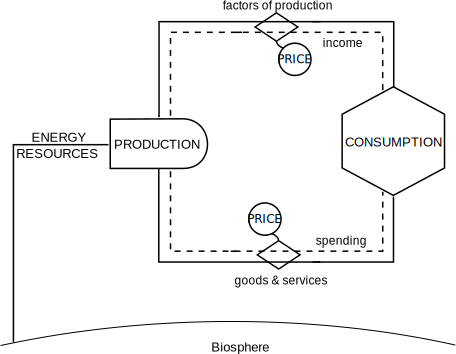
\includegraphics[width=\linewidth]{Part_0/Chapter_Introduction/images/Perpetual_motion_2.pdf}
\caption[The machine model]{The machine model of the economy includes
flows of energy into the economy from the biosphere.
This may be considered a perpetual motion machine 
of the second kind.}
\label{fig:perp_motion_2}
\end{figure}

The machine metaphor and engine model are still very much mechanistic.
Much like the engines of the Industrial Revolution,
the economic engine is assumed to be well-behaved and amenable to control.
Even today, machine metaphors abound in our economic discussions.
We speak of ``fueling'' the ``economic engine'' 
lest it should ``stall.''~\cite{Liu2012}
Like a well-running engine, the economy is assumed 
to be resilient to small or even quite large perturbations.  
It can either self-correct, 
or be corrected with adjustments to
a few predictable policy levers.

But, in light of the challenges discussed above,
how accurate is the engine model?

According to the Second Law of Thermodynamics,
all real-world processes involve the degradation
of material and especially energy resources
and the creation of entropy.
High quality (low entropy) material and energy come in;
low quality (high entropy) material and energy go out.
The depiction in Figure~\ref{fig:perp_motion_2} 
can be classified as a perpetual motion machine
of the \emph{second kind}:
it perfectly converts energy resources into 
work~(useful services) without generating
any entropy,
in violation of the Second Law of Thermodynamics.
Because the generation of high entropy~(low quality)
output is a \emph{necessary} feature of \emph{all} processes 
(including economic processes)
then the generation of wastes is a \emph{normal} feature of
economic processes,
not an anomaly.
Within a closed system, such as the earth,
these wastes soon accumulate,
necessitating the change to a ``spaceship'' economy,
wherein account is made of the waste outflows from
the economy.

We need a different model.


%%%%%%%%%% A new metaphor %%%%%%%%%%
\subsection{A new metaphor}
\label{sec:new_metaphor}
%%%%%%%%%% 

When our collective imagination is stuck on a metaphor that 
informs models in which the economy is isolated from or closed to the biosphere,
the suggestion to ``account for the environment'' is unconvincing, and 
the challenges cited earlier (natural resource extraction limits,
difficulty of material and energy substitutions, and 
exceeding the biosphere's waste assimilation capacity)
seem unimportant. 

Mounting evidence shows otherwise.

Thus, we need to find a new way to understand the complex, 
messy dynamics of real-world economies;
we need a new way to make sense of real-world events;
we need a new way to learn where and how economies can go wrong; and
we need to plan for the impending materials and energy transformations.
To do so, we had better be counting data to assess \emph{dynamic} models
guided by metaphors that tell us \emph{more} than ``the world is an orderly place.''
Our counting needs to be informed by metaphors and models that are
able to cope with rapid transience and transformation,
not just ordered stability.

We need a new metaphor.


%%%%%%%%%% An Apt Metaphor %%%%%%%%%%
\section{An apt metaphor for the economy}
\label{sec:apt_metaphor}
%%%%%%%%%%

If the clockwork and machine metaphors are unsuitable, 
what might an apt metaphor for the economy be?
And, if we find an apt metaphor, what types of models would it inform?
Furthermore, what data would the models tell us to collect?
That is, how should we go about accounting for the environment?
From here to Section~\ref{sec:our_new_model}, we answer the above questions
and, in the process, sketch the outline of our new approach 
to thinking about and accounting for materials, energy, and the economy.
Later chapters will flesh out this sketch.

To begin the search for an apt metaphor, 
we might first ask the question, 
what characteristics should the metaphor possess?
In our opinion, an apt metaphor should account for the facts 
that a real economy:

\begin{enumerate}
	\item{\label{itm:intake}intakes material and energy from the biosphere}
	\item{\label{itm:internal_exchange}exchanges materials, energy, and information internally}
	\item{\label{itm:discharge}discharges material and energy wastes to the biosphere}
	\item{\label{itm:energetic_costs}is affected by energetic costs}
	\item{\label{itm:scarcity}is affected non-linearly by scarcity 
			in the face of low substitutibility}
	\item{\label{itm:non-linear}can change non-linearly or in discrete steps with the potential 
			for structural transformation}
	\item{\label{itm:embodies}embodies energy in material stocks, and}
	\item{\label{itm:robust}maintains organizational structure despite changes 
			in the environment.\footnote{We note that 
				several areas of the literature speak to the items in this list.
				Material Flow Analysis~(MFA) and 
				Economy-Wide Material Flow Analys~(EW-MFA)
				stress the importance of
				material intake by the economy. 
				(See Section~\ref{sec:materials_auto}.)
				The Input-Output~(I-O) method highlights the effects of internal exchanges
				of material and information with economies. 
				(See Chapter~\ref{chap:intensity}.)
				Life-Cycle Assessment~(LCA) techniques focus attention 
				on otherwise-neglected wastes. 
				(See Section~\ref{sec:intensity_auto}.)
				Net Energy Analysis~(NEA) predicts that energy resource 
				scarcity reduces Energy Return on Investment~(EROI)
				and increases energy prices.
				(See Sections~\ref{sec:B_energy} 
				and~\ref{sec:resource_quality_and_irreversibility}.)
				The Energy Input-Output~(EI-O) method gives prominence to energetic costs
				for internal material and energy flows.
				(See Chapter~\ref{chap:intensity}.)
				And, thermodynamic control-volume modeling describes
				transient behavior and system transformations.
				(See Chapters~\ref{chap:materials}--\ref{chap:value}.)
			}}
\end{enumerate}

Living metabolisms\footnote{The 
	Greek root of metabolism 
	(\emph{metabol$\bar{e}$}) means ``change.''}
exhibit the characteristics in the list above.
Metabolisms and the organisms they support
are intimately connected with the biosphere:
they withdraw materials and energy from the biosphere~(\ref{itm:intake}), 
transfer materials and energy internally via metabolic processes~(\ref{itm:internal_exchange}),
and discharge wastes back to the biosphere~(\ref{itm:discharge});
in fact, their very survival depends on these processes.
Extending Figures~\ref{fig:perp_motion_1} and~\ref{fig:perp_motion_2}
to include the facts in items~(\ref{itm:intake})--(\ref{itm:discharge}), % chktex 36
we obtain Figure~\ref{fig:metabolic_economy}.
Metabolisms are affected by energetic costs~(\ref{itm:energetic_costs}): 
an organism that obtains less energy than it expends is doomed.
Withholding life-sustaining resources brings drastic, non-linear
consequences for any metabolism~(\ref{itm:scarcity}).
Metabolisms enable non-linear, structural transformations
in their host organisms (e.g., metamorphosis, puberty, and evolution)~(\ref{itm:non-linear}).
And, energy absorbed into a metabolism is considered to be ``embodied''
in the cells of the organism~(\ref{itm:embodies}).
Metabolisms exist in a state of dynamic stability~(\ref{itm:robust}),
adjusting and readjusting to maintain their internal conditions
despite changes in the environment;
for a metabolism, equilibrium means death!

The economy is society's metabolism.\cite{F-K1998, Giampietro2000, Giampietro2013}

\begin{figure}[!ht]
\centering\
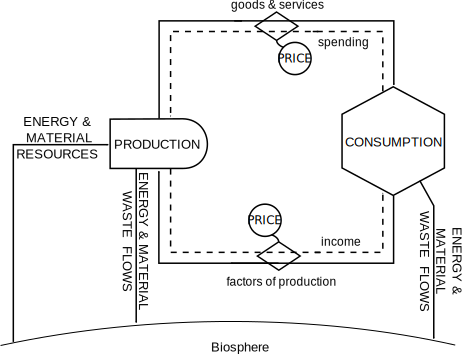
\includegraphics[width=\linewidth]{Part_0/Chapter_Introduction/images/PERKS.pdf}
\caption[The metabolism model]{The metabolism model provides a comprehensive view 
of the economy, fully consistent with the laws of thermodynamics, 
including degraded resources (waste) expelled 
to the environment as a necessary consequence of economic activity.}
\label{fig:metabolic_economy}
\end{figure}


%%%%%%%%%% Apt Models %%%%%%%%%%
\section{An apt material, energy, and economy model}
\label{sec:apt_models}
%%%%%%%%%%

As discussed in Section~\ref{sec:metaphors_and_models}, 
metaphors give rise to models.
So, a natural question is: 
``what types of models does the metabolism metaphor inform?''

In our opinion, apt models should have the following characteristics:

\begin{enumerate}
	\item{\label{itm:flows}account for flows of materials and energy 
			into, within, and out of the economy,}
	\item{\label{itm:accumulation}account for accumulation of materials and energy 
			within the economy,}
	\item{\label{itm:metrics}provide metrics that relate energy demands and economic value, and}
	\item{\label{itm:accounting}provide results that are comparable against existing 
			(or expanded) national accounting.}
\end{enumerate}

Material and energy flow balance equations, 
often employed by thermodynamicists, 
can account for both flows~(\ref{itm:flows}) and accumulation~(\ref{itm:accumulation}) 
of materials and energy within systems.
We will adapt an existing Input-Output~(I-O)
energy analysis method to develop a 
technique for obtaining metrics 
of energy and economic value~(\ref{itm:metrics}).\footnote{See Chapter~\ref{chap:intensity}
for details of the I-O method.}
Finally, we note that systems of national accounts use the economic sector
as their level of analysis. 
Thus, apt models should be also implemented at the economic sector level
so that model results can be 
compared against existing (or expanded) national accounting~(\ref{itm:accounting}).


%%%%%%%%%% Our new model %%%%%%%%%%
\section{Our new model}
\label{sec:our_new_model}
%%%%%%%%%%

%**** Add a discussion of the "system" and "boundaries". Discuss levels of disaggregation as a proxy for area of interest ****
%
%**** Emphasize the greater understanding that comes from explicitly modeling accumulation of (embodied) energy and materials within the economy. ****
%
%**** You have to draw boundaries somewhere.****
%
%**** We disaggregate the economy, because that the is the locus of our interest. An ecologist, in contrast, may choose to disaggregated the biosphere to answer questions such as biodiversity, etc. The biosphere is a container with which our system of interest is interacting. Why? An area of interest is the impact of energy transitions on the economy. ****

We contend that society is not accounting materials and energy adequately 
to prepare for the coming material and energy transformations 
**** MCD - metamorphosis? ****.
In Sections~\ref{sec:apt_metaphor} and~\ref{sec:apt_models} above,
we identified a metabolism as an apt metaphor and model for the economy 
to assist the process of developing the knowledge and analysis approaches
necessary to plan for the upcoming transitions.
Some elements of our approach are not new.
We're not the first to claim that a metabolism is an apt metaphor for the economy
(Section~\ref{sec:apt_metaphor}).~\cite{Barradas1936, F-K1998, Giampietro2000, Haberl2001, Daniels2001}
Nor are we the first to claim that an apt model for the economy 
involves material and energy flow equations 
applied at the level of economic sectors using an Input-Output framework.~\cite{G-R1975 ,G-R1979a, Lenzen1998, Hendrickson2006}

But, we are the first to comprehensively include accumulation
of materials and embodied energy in an accounting framework
based on existing systems of national accounts.
We contend that accounting for accumulation 
of materials and embodied energy in economic sectors is essential
for several reasons:

**** Mik, can you have a look at this list? Matt ****

\begin{itemize}
	\item{real economies convert raw materials extracted from the biosphere
		 	into engineered objects that accumulate,  
			embodied as the infrastructure of the economy;}
	\item{accumulated materials and infrastructure require further material and energy flows
			for their operation and maintenance,
			thereby placing additional material and energy demands on the biosphere;}
	\item{accumulated materials and infrastructure depreciate and need to be replaced,
		 	leading to additional material and energy demands on the biosphere,}
	\item{rapidly growing economies have large accumulation rates, 
			and accounting only for non-accumulating,
			consumptive (through-put) flows of material and energy 
			underestimates the energy demands of those economies.}
\end{itemize}

To include this accumulation of materials and embodied energy, 
we had to re-think the I-O framework starting from fundamental assumptions
and then re-derive the I-O accounting equations
to allow for accumulation, as shown in the following chapters. 
Thus, to our knowledge, we are the first 
to systematically derive the I-O equations to account for accumulation
in a thermodynamically-consistent manner.

To complete the outline and scope for our new model, 
the following subsections address
questions of system boundary and what must be counted.


%%%%%%%%%% System boundary %%%%%%%%%%
\subsection{System boundary}
\label{sec:system_boundary}
%%%%%%%%%% 

In Figure~\ref{fig:biosphere_economy},
the economy is shown as embedded within the surrounding environment,
the biosphere.
Materials and energy (yellow arrows) flow around the biosphere,
many of which do not interact with the economy.
Some of the flows are extracted from the biosphere for human purposes.
These flow around (and accumulate within) the economy,
before ultimately being emitted back into the biosphere as waste.
Processes within the biosphere are then able to regenerate some of these
flows making them available again for human use,
for example the conversion of carbon dioxide into oxygen by photosynthesis.

We have chosen to draw the system boundary of this new model around the economy
and focus only on those flows that pass through the economy.\footnote{An ecologist
	is likely have a different focus 
	and study material and energy flows that never enter the economy.
	}
This is the same system boundary used by the
systems of national accounts (SNA),
although the types of flows accounted are different.
As will be seen in later chapters,
the economy (as our main locus of interest) is further disaggregated 
to the level of industrial sectors.
Our primary interest in doing this is that it is important 
to know where materials and energy accumulate in understanding
the structure of our economies.
This will provide us a better model of the economy and
enable greater understanding of the structural transformation that lies ahead.

The biosphere is included in the model, but only at an aggregated level;
it is the container for the economy. 
We ignore material and energy flows that occur only within the biosphere,
but do not enter the economy.
This means that many important issues lie outside the scope of our new model. 
For example, questions of species loss and
bio-diversity remain outside of this system. 

**** MCD - WHICH VERSION OF THE FIGURE DO WE PREFER?? ****


\begin{figure}[!ht]
\centering\
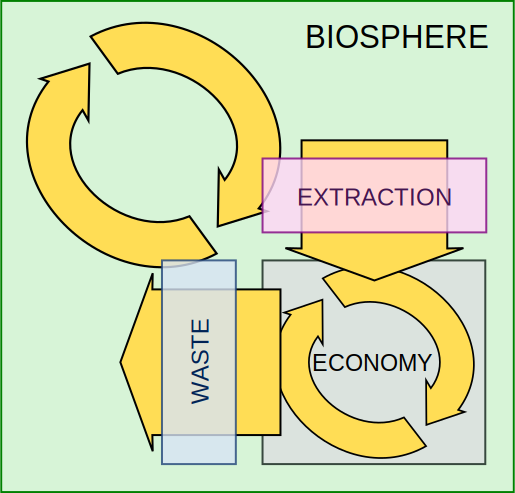
\includegraphics[width=\linewidth]{Part_0/Chapter_Introduction/images/Biosphere_economy.pdf}
\caption[The biosphere and the economy **** MCD - NEED A BETTER FIGURE TITLE ****]
				{The interaction of the economy with the biosphere.
				Materials and energy (yellow arrows) flow around the biosphere.
				Some flows are extracted for human use and enter the economy.
				The materials and energy flow around the economy 
				(as well as accumulating in capital stocks)
				before being emitted as wastes back into the biosphere.
				The size of the arrows does not indicate magnitude of flows.}
\label{fig:biosphere_economy}
\end{figure}

\begin{figure}[!ht]
\centering\
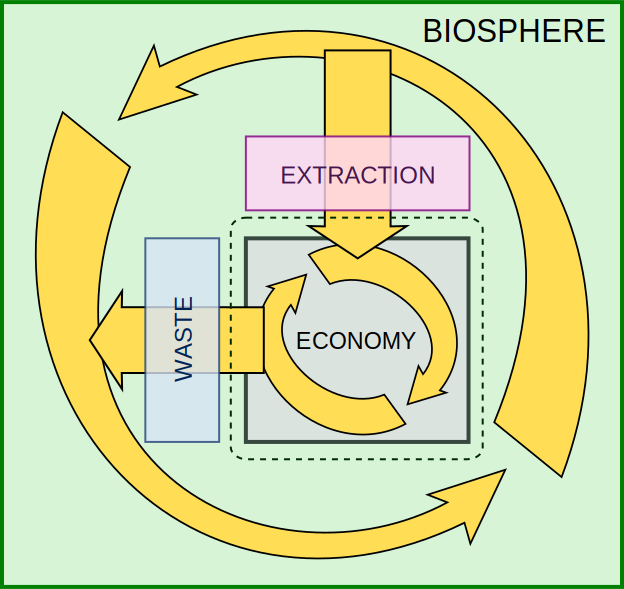
\includegraphics[width=\linewidth]{Part_0/Chapter_Introduction/images/Biosphere_economy_v2.pdf}
\caption[The biosphere and the economy **** MCD - NEED A BETTER FIGURE TITLE ****]
				{The interaction of the economy with the biosphere.
				Materials and energy (yellow arrows) flow around the biosphere.
				Some flows are extracted for human use and enter the economy.
				The materials and energy flow around the economy 
				(as well as accumulating in capital stocks)
				before being emitted as wastes back into the biosphere.
				The size of the arrows does not indicate magnitude of flows.}
\label{fig:biosphere_economy}
\end{figure}


%%%%%%%%%% What to count %%%%%%%%%%
\subsection{What to count}
\label{sec:what_to_count}
%%%%%%%%%% 

We believe the key to understanding how energy transformations will unfold
involves specifically understanding how

\begin{itemize}
	\item{materials,}
	\item{energy,}
	\item{embodied energy, and}
	\item{economic value}
\end{itemize}

\noindent{}each flow and accumulate within society's metabolism, the economy.
Of course, each of the above items interacts with the others 
and the biosphere dynamically.
If we can begin to carefully track these items, 
we will be on our way to gathering the information required to 
assist planning for upcoming materials and energy transformations.

A model informed by the metabolism metaphor may allow consumers, producers,
and policy-makers to answer critical questions that are not
answerable today. Example questions include:

\begin{enumerate}
	\item{What might be the optimal scale of an economy in terms of GDP 
			and what are the impacts of an optimally-sized economy on natural capital?}
    \item{How is fossil fuel dependency embedded in the interlocking fabric of the economy?} 
    \item{How will economies that are dependent on coal, oil, 
 			and other forms of non-renewable energy transition 
			to renewable forms of energy?}
	\item{How might an economy be affected as an increasing share of production
			is directed toward replacing 
			degraded ecosystem services?~\cite[p.~221]{kummel2011}​}
\end{enumerate}

To summarize Sections~\ref{sec:apt_metaphor}--\ref{sec:what_to_count}, 
our approach is to:

\begin{svgraybox}
	develop a dynamic model 
	by applying rigorous thermodynamics 
	to materials and energy flows into, among, 
	and out of economic sectors,
	informed by the metabolism metaphor,
	in a manner that is verifiable against 
	the existing (or expanded) 
	national accounts.
\end{svgraybox}

\noindent{}If successful, we will have developed an analysis framework 
that allows us to \emph{account for the environment}.


%%%%%%%%%% Structure %%%%%%%%%%
\section{Structure of the book}
\label{sec:structure}
%%%%%%%%%%

The bulleted list in Section~\ref{sec:what_to_count} 
provides the beginning of the structure for the rest of this book.

Part~\ref{part:matter} addresses flows of physical matter and energy
through the economy.
Chapter~\ref{chap:materials} discusses material flows and accumulation.
Flows of energy are covered in Chapter~\ref{chap:direct_energy}, 
and a rigorous, thermodynamics-based definition of and accounting for 
embodied energy is presented in Chapter~\ref{chap:embodied_energy}.

In Part~\ref{part:values}, we turn to flow and accumulation of 
non-physical entities through the economy. 
Flows and accumulation of economic value are discussed in Chapter~\ref{chap:value}.
In Chapter~\ref{chap:intensity}, we combine the results from 
Chapters~\ref{chap:embodied_energy} and~\ref{chap:value} to
calculate an important indicator of economic activity:
the energy intensity of economic production.

Part~\ref{part:implications} gives context to the framework developed in
Parts~\ref{part:matter}~and~\ref{part:values}.
Chapter~\ref{chap:implications} draws out some of the direct implications
of our framework.
Chapter~\ref{chap:unfinished_business} looks at 
unfinished business: practical, conceptual, and theoretical issues
that arise in the development of this framework.
And, we end with a summary in Chapter~\ref{chap:summary}.

\begin{table}
\caption[Examples used throughout this book]{Examples
used throughout this book.}
\begin{center}
  \begin{tabular}{c @{\hspace{1.5em}} c @{\hspace{1.5em}} c @{\hspace{1.5em}} c @{\hspace{1.5em}} c}
    \toprule
    Example & Sector 0 & Sector 1 & Sector 2 & Sector 3 \\ 
	\midrule
    A & Biosphere	&	Society            & NA         & NA                 \\
    B & Biosphere	&	Final Consumption  & Production & NA                 \\
    C & Biosphere	&	Final Consumption  & Energy     & Goods \& Services  \\
  \bottomrule
  \end{tabular}
\end{center}
\label{tab:examplesABC}
\end{table}
 
Throughout the methodological chapters~(\ref{chap:materials}--\ref{chap:intensity}),
our accounting framework is developed
through a series of increasingly-disaggregated
models of the economy~(Table~\ref{tab:examplesABC}),
and we use the US auto industry 
as a running example for application and discussion.

**** The next two paragraphs are duplicated from 
Section 2.5 (Materials in the US Auto Industry).
We duplicated them here temporarily so that the editors can 
see the purpose of and justification for the auto industry example. ****

The running example of the US auto industry demonstrates that our dynamic model 
can be tied into national accounts.
The US auto industry example shows where data are available 
(e.g., economic value, Chapter~\ref{chap:value}), 
where it is old (e.g., energy intensity, Chapter~\ref{chap:intensity}), 
and where it has never been available 
(e.g., accumulated embodied energy, Chapter~\ref{chap:embodied_energy}).  
The US auto industry is, therefore, 
illustrative of the challenges inherent 
in obtaining data that would feed the model.

The auto industry 
has been used previously
in the literature in both 
process-based~\cite{Berry:1973vo, Sullivan1995, Stodolsky1995, 
							Sullivan1998, McCleese2002, Sullivan2010, Hawkins2012}
and Input-Output~\cite{Bullard:1978vd, MacLean1998, MacLean2003}
analysis methods,
Furthermore, the industry
remains a large portion of many industrialized economies, 
is very resource intensive, 
has obvious links with energy because
its health is sensitive to disruptions in energy supplies, and
the industry also shows evidence of 
post-industrial decline (shrinking profit margins, etc.).

\bibliographystyle{unsrt}
\bibliography{../../Metabolic}


% Always give a unique label
% and use \ref{<label>} for cross-references
% and \cite{<label>} for bibliographic references
% use \sectionmark{}
% to alter or adjust the section heading in the running head
%% Instead of simply listing headings of different levels we recommend to let every heading be followed by at least a short passage of text. Furtheron please use the \LaTeX\ automatism for all your cross-references and citations.

%% Please note that the first line of text that follows a heading is not indented, whereas the first lines of all sequent paragraphs are.

%% Use the standard \verb|equation| environment to typeset your equations, e.g.
%
%% \begin{equation}
%% a \times b = c\;,
%% \end{equation}
%
%% however, for multiline equations we recommend to use the \verb|eqnarray|
%% environment\footnote{In physics texts please activate the class option \texttt{vecphys} to depict your vectors in \textbf{\itshape boldface-italic} type - as is customary for a wide range of physical jects.}.
%% \begin{eqnarray}
%% a \times b = c \nonumber\\
%% \vec{a} \cdot \vec{b}=\vec{c}
%% \label{eq:01}
%% \end{eqnarray}

%% \section{section Heading}
%% \label{sec:2}
%% Instead of simply listing headings of different levels we recommend to let every heading be followed by at least a short passage of text. Furtheron please use the \LaTeX\ automatism for all your cross-references\index{cross-references} and citations\index{citations} as has already been described in Sect.~\ref{sec:2}.

%% \begin{quotation}
%% Please do not use quotation marks when quoting texts! Simply use the \verb|quotation| environment -- it will automatically render Springer's preferred layout.
%% \end{quotation}


%% \section{section Heading}
%% Instead of simply listing headings of different levels we recommend to let every heading be followed by at least a short passage of text. Furtheron please use the \LaTeX\ automatism for all your cross-references and citations as has already been described in Sect.~\ref{sec:2}, see also Fig.~\ref{fig:1}\footnote{If you copy text passages, figures, or tables from other works, you must obtain \textit{permission} from the copyright holder (usually the original publisher). Please enclose the signed permission with the manucript. The sources\index{permission to print} must be acknowledged either in the captions, as footnotes or in a separate section of the book.}

%% Please note that the first line of text that follows a heading is not indented, whereas the first lines of all sequent paragraphs are.

% For figures use
%
%% \begin{figure}[b]
%% \sidecaption
% Use the relevant command for your figure-insertion program
% to insert the figure file.
% For example, with the option graphics use
%% \includegraphics[scale=.65]{figure}
%
% If not, use
%\picplace{5cm}{2cm} % Give the correct figure height and width in cm
%
%% \caption{If the width of the figure is less than 7.8 cm use the \texttt{sidecapion} command to flush the caption on the left side of the page. If the figure is positioned at the top of the page, align the sidecaption with the top of the figure -- to achieve this you simply need to use the optional argument \texttt{[t]} with the \texttt{sidecaption} command}
%% \label{fig:1}       % Give a unique label
%% \end{figure}


%% \paragraph{Paragraph Heading} %
%% Instead of simply listing headings of different levels we recommend to let every heading be followed by at least a short passage of text. Furtheron please use the \LaTeX\ automatism for all your cross-references and citations as has already been described in Sect.~\ref{sec:2}.

%% Please note that the first line of text that follows a heading is not indented, whereas the first lines of all sequent paragraphs are.

%% For typesetting numbered lists we recommend to use the \verb|enumerate| environment -- it will automatically render Springer's preferred layout.

%% \begin{enumerate}
%% \item{Livelihood and survival mobility are oftentimes coutcomes of uneven socioeconomic development.}
%% \begin{enumerate}
%% \item{Livelihood and survival mobility are oftentimes coutcomes of uneven socioeconomic development.}
%% \item{Livelihood and survival mobility are oftentimes coutcomes of uneven socioeconomic development.}
%% \end{enumerate}
%% \item{Livelihood and survival mobility are oftentimes coutcomes of uneven socioeconomic development.}
%% \end{enumerate}


%% \paragraph{paragraph Heading} In order to avoid simply listing headings of different levels we recommend to let every heading be followed by at least a short passage of text. Use the \LaTeX\ automatism for all your cross-references and citations as has already been described in Sect.~\ref{sec:2}, see also Fig.~\ref{fig:2}.

%% Please note that the first line of text that follows a heading is not indented, whereas the first lines of all sequent paragraphs are.

%% For unnumbered list we recommend to use the \verb|itemize| environment -- it will automatically render Springer's preferred layout.

%% \begin{itemize}
%% \item{Livelihood and survival mobility are oftentimes coutcomes of uneven socioeconomic development, cf. Table~\ref{tab:1}.}
%% \begin{itemize}
%% \item{Livelihood and survival mobility are oftentimes coutcomes of uneven socioeconomic development.}
%% \item{Livelihood and survival mobility are oftentimes coutcomes of uneven socioeconomic development.}
%% \end{itemize}
%% \item{Livelihood and survival mobility are oftentimes coutcomes of uneven socioeconomic development.}
%% \end{itemize}

%% \begin{figure}[t]
%% \sidecaption[t]
% Use the relevant command for your figure-insertion program
% to insert the figure file.
% For example, with the option graphics use
%% \includegraphics[scale=.65]{figure}
%
% If not, use
%\picplace{5cm}{2cm} % Give the correct figure height and width in cm
%
%% \caption{Please write your figure caption here}
%% \label{fig:2}       % Give a unique label
%% \end{figure}

%% \runinhead{Run-in Heading Boldface Version} Use the \LaTeX\ automatism for all your cross-references and citations as has already been described in Sect.~\ref{sec:2}.

%% \runinhead{Run-in Heading Italic Version} Use the \LaTeX\ automatism for all your cross-refer\-ences and citations as has already been described in Sect.~\ref{sec:2}\index{paragraph}.
% Use the \index{} command to code your index words
%
% For tables use
%
%% \begin{table}
%% \caption{Please write your table caption here}
%% \label{tab:1}       % Give a unique label
%
% For LaTeX tables use
%
%% \begin{tabular}{p{2cm}p{2.4cm}p{2cm}p{4.9cm}}
%% \hline\noalign{\smallskip}
%% Classes & class & Length & Action Mechanism  \\
%% \noalign{\smallskip}\svhline\noalign{\smallskip}
%% Translation & mRNA$^a$  & 22 (19--25) & Translation repression, mRNA cleavage\\
%% Translation & mRNA cleavage & 21 & mRNA cleavage\\
%% Translation & mRNA  & 21--22 & mRNA cleavage\\
%%Translation & mRNA  & 24--26 & Histone and DNA Modification\\
%%\noalign{\smallskip}\hline\noalign{\smallskip}
%%\end{tabular}
%%$^a$ Table foot note (with superscript)
%%\end{table}
%
%% \section{Section Heading}
%%\label{sec:3}
% Always give a unique label
% and use \ref{<label>} for cross-references
% and \cite{<label>} for bibliographic references
% use \sectionmark{}
% to alter or adjust the section heading in the running head
%% Instead of simply listing headings of different levels we recommend to let every heading be followed by at least a short passage of text. Furtheron please use the \LaTeX\ automatism for all your cross-references and citations as has already been described in Sect.~\ref{sec:2}.

%% Please note that the first line of text that follows a heading is not indented, whereas the first lines of all sequent paragraphs are.

%%If you want to list definitions or the like we recommend to use the Springer-enhanced \verb|description| environment -- it will automatically render Springer's preferred layout.

%%\begin{description}[Type 1]
%%\item[Type 1]{That addresses central themes pertainng to migration, health, and disease. In Sect.~\ref{sec:1}, Wilson discusses the role of human migration in infectious disease distributions and patterns.}
%%\item[Type 2]{That addresses central themes pertainng to migration, health, and disease. In Sect.~\ref{sec:2}, Wilson discusses the role of human migration in infectious disease distributions and patterns.}
%%\end{description}

%%\section{section Heading} %
%% In order to avoid simply listing headings of different levels we recommend to let every heading be followed by at least a short passage of text. Use the \LaTeX\ automatism for all your cross-references and citations citations as has already been described in Sect.~\ref{sec:2}.

%% Please note that the first line of text that follows a heading is not indented, whereas the first lines of all sequent paragraphs are.

%% \begin{svgraybox}
%% If you want to emphasize complete paragraphs of texts we recommend to use the newly defined Springer class option \verb|graybox| and the newly defined environment \verb|svgraybox|. This will produce a 15 percent screened box 'behind' your text.

%% If you want to emphasize complete paragraphs of texts we recommend to use the newly defined Springer class option and environment \verb|svgraybox|. This will produce a 15 percent screened box 'behind' your text.
%% \end{svgraybox}


%% \section{section Heading}
%%Instead of simply listing headings of different levels we recommend to let every heading be followed by at least a short passage of text. Furtheron please use the \LaTeX\ automatism for all your cross-references and citations as has already been described in Sect.~\ref{sec:2}.

%% Please note that the first line of text that follows a heading is not indented, whereas the first lines of all sequent paragraphs are.

%% \begin{theorem}
%% Theorem text goes here.
%% \end{theorem}
%
% or
%
%% \begin{definition}
%% Definition text goes here.
%% \end{definition}

%% \begin{proof}
%\smartqed
%% Proof text goes here.
%% \qed
%% \end{proof}

%%\paragraph{Paragraph Heading} %
%% Instead of simply listing headings of different levels we recommend to let every heading be followed by at least a short passage of text. Furtheron please use the \LaTeX\ automatism for all your cross-references and citations as has already been described in Sect.~\ref{sec:2}.

%% Note that the first line of text that follows a heading is not indented, whereas the first lines of all subsequent paragraphs are.
%
% For built-in environments use
%
%%\begin{theorem}
%%Theorem text goes here.
%%\end{theorem}
%
%%\begin{definition}
%%Definition text goes here.
%%\end{definition}
%
%%\begin{proof}
%%\smartqed
%% Proof text goes here.
%%\qed
%%\end{proof}
%
%% \begin{acknowledgement}
%% If you want to include acknowledgments of assistance and the like at the end of an individual chapter please use the \verb|acknowledgement| environment -- it will automatically render Springer's preferred layout.
%% \end{acknowledgement}
%
%% \section*{Appendix}
%% \addcontentsline{toc}{section}{Appendix}
%
%% When placed at the end of a chapter or contribution (as opposed to at the end of the book), the numbering of tables, figures, and equations in the appendix section continues on from that in the main text. Hence please \textit{do not} use the \verb|appendix| command when writing an appendix at the end of your chapter or contribution. If there is only one the appendix is designated ``Appendix'', or ``Appendix 1'', or ``Appendix 2'', etc. if there is more than one.

%% \begin{equation}
%% a \times b = c
%% \end{equation}
% Problems or Exercises should be sorted chapterwise
%% \section*{Problems}
%% \addcontentsline{toc}{section}{Problems}
%
% Use the following environment.
% Don't forget to label each problem;
% the label is needed for the solutions' environment
%% \begin{prob}
%% \label{prob1}
%% A given problem or Excercise is described here. The
%% problem is described here. The problem is described here.
%% \end{prob}

%% \begin{prob}
%% \label{prob2}
%% \textbf{Problem Heading}\\
%% (a) The first part of the problem is described here.\\
%% (b) The second part of the problem is described here.
%% \end{prob}




%%%%%%%%%%%%%%%%%%%%% chapter.tex %%%%%%%%%%%%%%%%%%%%%%%%%%%%%%%%%
%
% sample chapter
%
% Use this file as a template for your own input.
%
%%%%%%%%%%%%%%%%%%%%%%%% Springer-Verlag %%%%%%%%%%%%%%%%%%%%%%%%%%
%\motto{Use the template \emph{chapter.tex} to style the various elements of your chapter content.}
\chapter{Methodology}
\chaptermark{Methodology}
\label{chap:meth} % Always give a unique label
% use \chaptermark{}
% to alter or adjust the chapter heading in the running head

\abstract*{[NEED TO ADD ABSTRACT HERE]}

%% \abstract{Each chapter should be preceded by an abstract (10--15 lines long) that summarizes the content. The abstract will appear \textit{online} at \url{www.SpringerLink.com} and be available with unrestricted access. This allows unregistered users to read the abstract as a teaser for the complete chapter. As a general rule the abstracts will not appear in the printed version of your book unless it is the style of your particular book or that of the series to which your book belongs.\newline\indent
%% Please use the 'starred' version of the new Springer \texttt{abstract} command for typesetting the text of the online abstracts (cf. source file of this chapter template \texttt{abstract}) and include them with the source files of your manuscript. Use the plain \texttt{abstract} command if the abstract is also to appear in the printed version of the book.}

%% Use the template \emph{chapter.tex} together with the Springer document class SVMono (monograph-type books) or SVMult (edited books) to style the various elements of your chapter content in the Springer layout.

%%%%%%%%%% Methodology %%%%%%%%%%
\section{Model economy}
%%%%%%%%%%

The model economy employed herein consists of sectors that produce a single product, either an energy product (energy sectors) or other goods and services (non-energy sectors). Economic sectors receive as inputs direct energy ($E$) and materials in which energy is embodied ($B$).\footnote{A formal definition for embodied energy ($B$) is presented in Section \ref{sec:embodied_energy}.} Economic sectors emit waste heat ($Q$).

%%%%%%%%%% Methodology %%%%%%%%%%
\section{Direct energy ($E$), indirect (embodied) energy ($B$), and waste heat ($Q$)}
%%%%%%%%%%

We distinguish between direct energy resources ($E$), such as coal or oil, and indirect energy ($B$) ``embodied'' in outputs from economic sectors. $E$ represents the energetic value of an energy resource (measured as heating value, chemical potential energy, or exergy). In contrast, $B$ represents the energy expended in the production and delivery of goods in the economy, and, as such, measures accumulated upstream energy consumption from the network of economic sectors within the economy. `Indirect' energy and `embodied' energy are synonyms. Both $E$ and $B$ are measured in energy units (joules or BTUs). The flow rates of direct energy ($\dot{E}$) and indirect energy ($\dot{B}$) among sectors of the economy, the Earth, and society are in units of power (energy per unit time, J/time or BTU/time).

Waste heat ($\dot{Q}$) flows from sectors of the economy and society to the Earth and its atmosphere, the necessary result of inefficient consumption of direct energy $E$. Like $\dot{E}$ and $\dot{B}$, the units of $\dot{Q}$ are energy per unit time.

\begin{figure}[H]
\includegraphics[width=0.8\linewidth]{Chapter_Methodology/images/Basic_unit_v5.pdf}
\caption{The basic unit of input-output modeling: A) the standard economic approach includes only transactions among sectors of the economy; B) the ecological economics approach models inputs from the natural environment outside the economy as factors of production and; C) the method presented here accounts also for accumulation, K, of embodied energy within materials in economic sectors.}
\label{fig:basic_unit}
\end{figure}

%%%%%%%%%% Methodology %%%%%%%%%%
\section{Total energy ($T$)}
%%%%%%%%%%

Total energy ($T$) is the sum of the direct and indirect (embodied) energy.

\begin{equation} \label{eq:T_def}
	T \equiv E + B
\end{equation}

In general, the flow rate of total energy among sectors in the economy, the earth, and society is given by

\begin{equation} \label{eq:T_dot_def}
	\dot{T} = \dot{E} + \dot{B}.
\end{equation}

In some cases, total energy flows may consist of direct energy ($\dot{E}$) or embodied energy ($\dot{B}$) exclusively. For example, the flow of extracted crude oil from the earth consists of direct energy only ($\dot{B} = 0$ and $\dot{T} = \dot{E}$), because, in this method, no embodied energy ($B$) has been added to the crude oil until it reaches the downstream side of the pump. The flow of goods produced by a non-energy sector of the economy consists of indirect energy only ($\dot{E} = 0$, and therefore $\dot{T} = \dot{B}$), because no direct energy ($E$) is produced by a non-energy sector in this model economy. 

In other cases, total energy flows may have both direct \emph{and} indirect components. For example, the flow of refined petroleum from the energy sector has both a direct energy ($\dot{E}$, the energy content of the oil product, usually represented by chemical potential energy) and embodied energy ($\dot{B}$, which accounts for the energy consumed in upstream processes to extract and refine the crude oil).\footnote{Outputs from agricultural sectors will be similar: both the direct energy component (comprising chemical potential energy) and the embodied energy component will be non-zero.}

Single subscripts on $T$, $E$, or $B$ can mean one of two things: $\dot{T}_{i}$ indicates the outflow of total energy from sector $i$, whereas $T_{i}$ denotes the total energy content of sector $i$. Double subscripts on $T$, $E$, or $B$ (e.g., $\dot{T}_{ij}$) indicate a flow from sector $i$ to sector $j$,\footnote{In the following discussion, the first index always indicates the sector \emph{from} which a quantity flows, and the second index indicates the sector \emph{to} which a quantity flows.} in this case for total energy ($T$).  

The I-O literature \cite{Bullard1975, Herendeen1978} [REF TO BULLARD AND HERENDEEN, ETC. HERE --MKH] assumes (a) that steady state conditions exist (i.e., no accumulation of total energy in economic sectors) and (b) that flows of total energy ($\dot{T}$) are \emph{conserved}, where by \emph{conserved}, it is meant that total energy can be neither created nor destroyed. Like the literature, we assume that total energy is conserved. However, we depart from the literature to allow durability of goods as represented by total energy accumulation in economic sectors. Steady state, this approach is not.

Total energy may accumulate within an economic sector as stocks of direct energy materials (piles of coal or tanks of oil) but also as embodied energy in stocks of capital goods (e.g. machinery or buildings). The rate of accumulation of total energy ($\frac{dT}{dt}$) in a sector of the economy, the Earth, or society is given by the time derivative of total energy:

\begin{equation} \label{eq:T_accum_def}
	\frac{\mathrm{d}T}{\mathrm{d}t} = \frac{\mathrm{d}E}{\mathrm{d}t} + \frac{\mathrm{d}B}{\mathrm{d}t}.
\end{equation}

We note that the definition of total energy (Equation \ref{eq:T_def}) includes direct energy ($E$) and embodied energy ($B$) terms. On the other hand, the First Law of Thermodynamics includes direct energy ($E$) and waste heat ($Q$) terms. The consequence of the foregoing difference is that an interesting relationship exists between embodied energy ($B$) and waste heat ($Q$). We shall see in the following example that waste heat from an economic sector can be considered to contribute to energy embodied within the products of that sector.


\bibliography{EROI_review_v2}
\bibliographystyle{unsrt}


% Always give a unique label
% and use \ref{<label>} for cross-references
% and \cite{<label>} for bibliographic references
% use \sectionmark{}
% to alter or adjust the section heading in the running head
%% Instead of simply listing headings of different levels we recommend to let every heading be followed by at least a short passage of text. Furtheron please use the \LaTeX\ automatism for all your cross-references and citations.

%% Please note that the first line of text that follows a heading is not indented, whereas the first lines of all subsequent paragraphs are.

%% Use the standard \verb|equation| environment to typeset your equations, e.g.
%
%% \begin{equation}
%% a \times b = c\;,
%% \end{equation}
%
%% however, for multiline equations we recommend to use the \verb|eqnarray|
%% environment\footnote{In physics texts please activate the class option \texttt{vecphys} to depict your vectors in \textbf{\itshape boldface-italic} type - as is customary for a wide range of physical subjects.}.
%% \begin{eqnarray}
%% a \times b = c \nonumber\\
%% \vec{a} \cdot \vec{b}=\vec{c}
%% \label{eq:01}
%% \end{eqnarray}

%% \subsection{Subsection Heading}
%% \label{subsec:2}
%% Instead of simply listing headings of different levels we recommend to let every heading be followed by at least a short passage of text. Furtheron please use the \LaTeX\ automatism for all your cross-references\index{cross-references} and citations\index{citations} as has already been described in Sect.~\ref{sec:2}.

%% \begin{quotation}
%% Please do not use quotation marks when quoting texts! Simply use the \verb|quotation| environment -- it will automatically render Springer's preferred layout.
%% \end{quotation}


%% \subsubsection{Subsubsection Heading}
%% Instead of simply listing headings of different levels we recommend to let every heading be followed by at least a short passage of text. Furtheron please use the \LaTeX\ automatism for all your cross-references and citations as has already been described in Sect.~\ref{subsec:2}, see also Fig.~\ref{fig:1}\footnote{If you copy text passages, figures, or tables from other works, you must obtain \textit{permission} from the copyright holder (usually the original publisher). Please enclose the signed permission with the manucript. The sources\index{permission to print} must be acknowledged either in the captions, as footnotes or in a separate section of the book.}

%% Please note that the first line of text that follows a heading is not indented, whereas the first lines of all subsequent paragraphs are.

% For figures use
%
%% \begin{figure}[b]
%% \sidecaption
% Use the relevant command for your figure-insertion program
% to insert the figure file.
% For example, with the option graphics use
%% \includegraphics[scale=.65]{figure}
%
% If not, use
%\picplace{5cm}{2cm} % Give the correct figure height and width in cm
%
%% \caption{If the width of the figure is less than 7.8 cm use the \texttt{sidecapion} command to flush the caption on the left side of the page. If the figure is positioned at the top of the page, align the sidecaption with the top of the figure -- to achieve this you simply need to use the optional argument \texttt{[t]} with the \texttt{sidecaption} command}
%% \label{fig:1}       % Give a unique label
%% \end{figure}


%% \paragraph{Paragraph Heading} %
%% Instead of simply listing headings of different levels we recommend to let every heading be followed by at least a short passage of text. Furtheron please use the \LaTeX\ automatism for all your cross-references and citations as has already been described in Sect.~\ref{sec:2}.

%% Please note that the first line of text that follows a heading is not indented, whereas the first lines of all subsequent paragraphs are.

%% For typesetting numbered lists we recommend to use the \verb|enumerate| environment -- it will automatically render Springer's preferred layout.

%% \begin{enumerate}
%% \item{Livelihood and survival mobility are oftentimes coutcomes of uneven socioeconomic development.}
%% \begin{enumerate}
%% \item{Livelihood and survival mobility are oftentimes coutcomes of uneven socioeconomic development.}
%% \item{Livelihood and survival mobility are oftentimes coutcomes of uneven socioeconomic development.}
%% \end{enumerate}
%% \item{Livelihood and survival mobility are oftentimes coutcomes of uneven socioeconomic development.}
%% \end{enumerate}


%% \subparagraph{Subparagraph Heading} In order to avoid simply listing headings of different levels we recommend to let every heading be followed by at least a short passage of text. Use the \LaTeX\ automatism for all your cross-references and citations as has already been described in Sect.~\ref{sec:2}, see also Fig.~\ref{fig:2}.

%% Please note that the first line of text that follows a heading is not indented, whereas the first lines of all subsequent paragraphs are.

%% For unnumbered list we recommend to use the \verb|itemize| environment -- it will automatically render Springer's preferred layout.

%% \begin{itemize}
%% \item{Livelihood and survival mobility are oftentimes coutcomes of uneven socioeconomic development, cf. Table~\ref{tab:1}.}
%% \begin{itemize}
%% \item{Livelihood and survival mobility are oftentimes coutcomes of uneven socioeconomic development.}
%% \item{Livelihood and survival mobility are oftentimes coutcomes of uneven socioeconomic development.}
%% \end{itemize}
%% \item{Livelihood and survival mobility are oftentimes coutcomes of uneven socioeconomic development.}
%% \end{itemize}

%% \begin{figure}[t]
%% \sidecaption[t]
% Use the relevant command for your figure-insertion program
% to insert the figure file.
% For example, with the option graphics use
%% \includegraphics[scale=.65]{figure}
%
% If not, use
%\picplace{5cm}{2cm} % Give the correct figure height and width in cm
%
%% \caption{Please write your figure caption here}
%% \label{fig:2}       % Give a unique label
%% \end{figure}

%% \runinhead{Run-in Heading Boldface Version} Use the \LaTeX\ automatism for all your cross-references and citations as has already been described in Sect.~\ref{sec:2}.

%% \subruninhead{Run-in Heading Italic Version} Use the \LaTeX\ automatism for all your cross-refer\-ences and citations as has already been described in Sect.~\ref{sec:2}\index{paragraph}.
% Use the \index{} command to code your index words
%
% For tables use
%
%% \begin{table}
%% \caption{Please write your table caption here}
%% \label{tab:1}       % Give a unique label
%
% For LaTeX tables use
%
%% \begin{tabular}{p{2cm}p{2.4cm}p{2cm}p{4.9cm}}
%% \hline\noalign{\smallskip}
%% Classes & Subclass & Length & Action Mechanism  \\
%% \noalign{\smallskip}\svhline\noalign{\smallskip}
%% Translation & mRNA$^a$  & 22 (19--25) & Translation repression, mRNA cleavage\\
%% Translation & mRNA cleavage & 21 & mRNA cleavage\\
%% Translation & mRNA  & 21--22 & mRNA cleavage\\
%%Translation & mRNA  & 24--26 & Histone and DNA Modification\\
%%\noalign{\smallskip}\hline\noalign{\smallskip}
%%\end{tabular}
%%$^a$ Table foot note (with superscript)
%%\end{table}
%
%% \section{Section Heading}
%%\label{sec:3}
% Always give a unique label
% and use \ref{<label>} for cross-references
% and \cite{<label>} for bibliographic references
% use \sectionmark{}
% to alter or adjust the section heading in the running head
%% Instead of simply listing headings of different levels we recommend to let every heading be followed by at least a short passage of text. Furtheron please use the \LaTeX\ automatism for all your cross-references and citations as has already been described in Sect.~\ref{sec:2}.

%% Please note that the first line of text that follows a heading is not indented, whereas the first lines of all subsequent paragraphs are.

%%If you want to list definitions or the like we recommend to use the Springer-enhanced \verb|description| environment -- it will automatically render Springer's preferred layout.

%%\begin{description}[Type 1]
%%\item[Type 1]{That addresses central themes pertainng to migration, health, and disease. In Sect.~\ref{sec:1}, Wilson discusses the role of human migration in infectious disease distributions and patterns.}
%%\item[Type 2]{That addresses central themes pertainng to migration, health, and disease. In Sect.~\ref{subsec:2}, Wilson discusses the role of human migration in infectious disease distributions and patterns.}
%%\end{description}

%%\subsection{Subsection Heading} %
%% In order to avoid simply listing headings of different levels we recommend to let every heading be followed by at least a short passage of text. Use the \LaTeX\ automatism for all your cross-references and citations citations as has already been described in Sect.~\ref{sec:2}.

%% Please note that the first line of text that follows a heading is not indented, whereas the first lines of all subsequent paragraphs are.

%% \begin{svgraybox}
%% If you want to emphasize complete paragraphs of texts we recommend to use the newly defined Springer class option \verb|graybox| and the newly defined environment \verb|svgraybox|. This will produce a 15 percent screened box 'behind' your text.

%% If you want to emphasize complete paragraphs of texts we recommend to use the newly defined Springer class option and environment \verb|svgraybox|. This will produce a 15 percent screened box 'behind' your text.
%% \end{svgraybox}


%% \subsubsection{Subsubsection Heading}
%%Instead of simply listing headings of different levels we recommend to let every heading be followed by at least a short passage of text. Furtheron please use the \LaTeX\ automatism for all your cross-references and citations as has already been described in Sect.~\ref{sec:2}.

%% Please note that the first line of text that follows a heading is not indented, whereas the first lines of all subsequent paragraphs are.

%% \begin{theorem}
%% Theorem text goes here.
%% \end{theorem}
%
% or
%
%% \begin{definition}
%% Definition text goes here.
%% \end{definition}

%% \begin{proof}
%\smartqed
%% Proof text goes here.
%% \qed
%% \end{proof}

%%\paragraph{Paragraph Heading} %
%% Instead of simply listing headings of different levels we recommend to let every heading be followed by at least a short passage of text. Furtheron please use the \LaTeX\ automatism for all your cross-references and citations as has already been described in Sect.~\ref{sec:2}.

%% Note that the first line of text that follows a heading is not indented, whereas the first lines of all subsequent paragraphs are.
%
% For built-in environments use
%
%%\begin{theorem}
%%Theorem text goes here.
%%\end{theorem}
%
%%\begin{definition}
%%Definition text goes here.
%%\end{definition}
%
%%\begin{proof}
%%\smartqed
%% Proof text goes here.
%%\qed
%%\end{proof}
%
%% \begin{acknowledgement}
%% If you want to include acknowledgments of assistance and the like at the end of an individual chapter please use the \verb|acknowledgement| environment -- it will automatically render Springer's preferred layout.
%% \end{acknowledgement}
%
%% \section*{Appendix}
%% \addcontentsline{toc}{section}{Appendix}
%
%% When placed at the end of a chapter or contribution (as opposed to at the end of the book), the numbering of tables, figures, and equations in the appendix section continues on from that in the main text. Hence please \textit{do not} use the \verb|appendix| command when writing an appendix at the end of your chapter or contribution. If there is only one the appendix is designated ``Appendix'', or ``Appendix 1'', or ``Appendix 2'', etc. if there is more than one.

%% \begin{equation}
%% a \times b = c
%% \end{equation}
% Problems or Exercises should be sorted chapterwise
%% \section*{Problems}
%% \addcontentsline{toc}{section}{Problems}
%
% Use the following environment.
% Don't forget to label each problem;
% the label is needed for the solutions' environment
%% \begin{prob}
%% \label{prob1}
%% A given problem or Excercise is described here. The
%% problem is described here. The problem is described here.
%% \end{prob}

%% \begin{prob}
%% \label{prob2}
%% \textbf{Problem Heading}\\
%% (a) The first part of the problem is described here.\\
%% (b) The second part of the problem is described here.
%% \end{prob}




%%%%%%%%%%%%%%%%%%%%% chapter.tex %%%%%%%%%%%%%%%%%%%%%%%%%%%%%%%%%
%
% sample chapter
%
% Use this file as a template for your own input.
%
%%%%%%%%%%%%%%%%%%%%%%%% Springer-Verlag %%%%%%%%%%%%%%%%%%%%%%%%%%
%\motto{Use the template \emph{chapter.tex} to style the various elements of your chapter content.}
\chapter{Example A: single sector economy}
\chaptermark{Example A}
\label{chap:single_sector} % Always give a unique label
% use \chaptermark{}
% to alter or adjust the chapter heading in the running head

\abstract*{[NEED TO ADD ABSTRACT HERE]}

%% \abstract{Each chapter should be preceded by an abstract (10--15 lines long) that summarizes the content. The abstract will appear \textit{online} at \url{www.SpringerLink.com} and be available with unrestricted access. This allows unregistered users to read the abstract as a teaser for the complete chapter. As a general rule the abstracts will not appear in the printed version of your book unless it is the style of your particular book or that of the series to which your book belongs.\newline\indent
%% Please use the 'starred' version of the new Springer \texttt{abstract} command for typesetting the text of the online abstracts (cf. source file of this chapter template \texttt{abstract}) and include them with the source files of your manuscript. Use the plain \texttt{abstract} command if the abstract is also to appear in the printed version of the book.}

%% Use the template \emph{chapter.tex} together with the Springer document class SVMono (monograph-type books) or SVMult (edited books) to style the various elements of your chapter content in the Springer layout.

In this section, we present an example economic analysis using a single-sector economy wherein the economy and society are merged together.

Figure \ref{fig:single_sector_flows_0} shows a single-sector Economy (represented by ``economy/society,'' 2) that extracts direct energy from the earth ($\dot{E}_{12}$). Direct energy and waste heat flows are identified by vectors. No direct energy flows from the economy (2) to the earth (1), only waste heat ($\dot{Q}_{21}$).

\begin{figure}[h!]
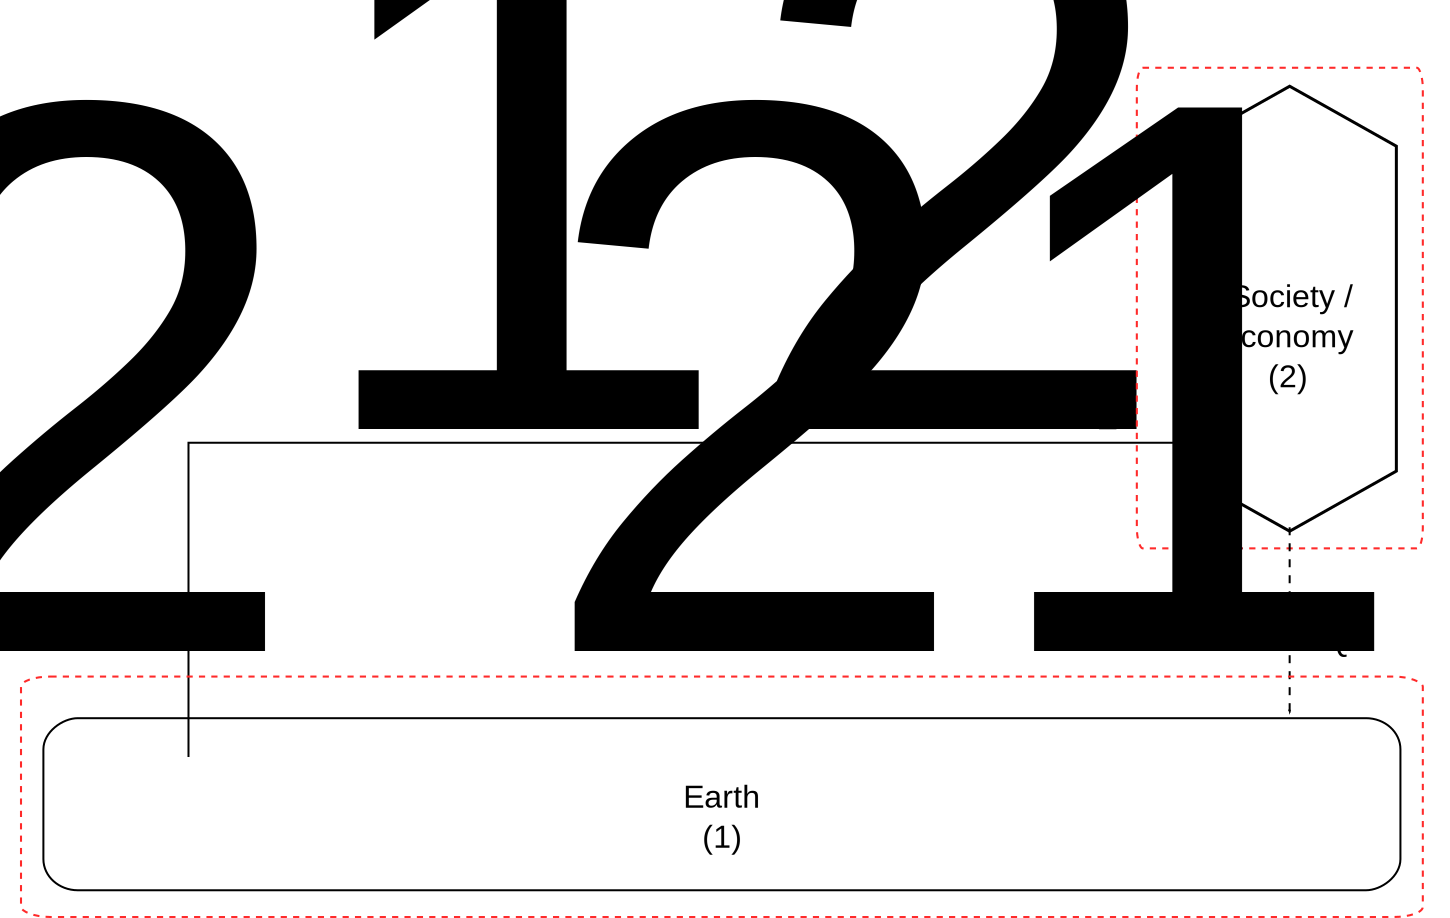
\includegraphics[width=1.0\linewidth]{Chapter_Example_A/images/I-O_one_sector_direct_energy.pdf}
\caption{Direct energy ($\dot{E}$) and waste heat ($\dot{Q}$) flows for a single-sector economy. }
\label{fig:single_sector_flows_0}
\end{figure}

%%%%%%%%%% Example A %%%%%%%%%%
\section{First Law of Thermodynamics}
%%%%%%%%%%

Both direct energy ($\dot{E}$, such as the energy content of coal, oil, and electricity), and waste heat ($\dot{Q}$) are accounted by the First Law of Thermodynamics. Accounting for possible accumulation of direct energy in the economy, the First Law of Thermodynamics indicates that

\begin{equation} \label{eq:dE_2/dt_single_sector}
	\frac{\mathrm{d}E_{2}}{\mathrm{d}t} = \dot{E}_{12} - \dot{Q}_{21}.
\end{equation}

Aside from, for example, the U.S. Strategic Petroleum Reserve, we are not stockpiling oil and coal at any meaningful rate, i.e. we consume fossil fuels at a rate equal to the extraction rate. Thus, the world is not accumulating direct energy in the economy.\footnote{A counter-example could be made for nuclear fuels where `spent' fuel represents a large exergetic stockpile, however, this reserve is not (presently) economically useful.} (The world \emph{is}, however, accumulating embodied energy in the economy as we shall see shortly.) Thus, the accumulation rate for direct energy $\left(\frac{\mathrm{d}E_{2}}{\mathrm{d}t}\right)$ in the above equation can be set to zero to obtain

\begin{equation} \label{eq:single_sector_direct_energy_no_accumulation}
	0 = \dot{E}_{12} - \dot{Q}_{21}.
\end{equation}

%%%%%%%%%% Example A %%%%%%%%%%
\section{Total energy accounting}
%%%%%%%%%%

Figure \ref{fig:single_sector_flows_2} shows the flows of total energy ($\dot{T}$) through the single-sector economy.

\begin{figure}[h!]
\includegraphics[width=1.0\linewidth]{Chapter_Example_A/images/I-O_one_sector_total_energy.pdf}
\caption{Total Energy Flows ($\dot{T}$) in a Single-sector Economy.}
\label{fig:single_sector_flows_2}
\end{figure}

We follow the I-O literature in assuming that total energy ($T$) is conserved. The I-O literature assumes steady-state operation of the economy with no accumulation of embodied energy in the economic sectors. (We will see later how the assumption in the literature introduces errors into I-O analyses.) We depart from the I-O literature by accounting for both accumulation and depreciation of energy embodied in sectors of the economy and society. By doing so, the present analysis does \emph{not} assume a steady-state economy. A total energy accounting around the single-sector economy (2) gives

\begin{equation} \label{eq:single_sector_T_with_accumulation}
	\frac{\mathrm{d}T_{2}}{\mathrm{d}t} = \dot{T}_{12}  - \dot{T}_{21}.
\end{equation}

%%%%%%%%%% Example A %%%%%%%%%%
\section{Embodied energy accounting}
%%%%%%%%%%

The First Law of Thermodynamics accounts for both direct energy ($E$) and waste heat ($Q$), whereas total energy ($T$) accounting tracks direct energy ($E$) and embodied energy ($B$). If we substitute the First Law into the total energy accounting equation, we can eliminate direct energy ($E$) to arrive at an embodied energy accounting equation. We begin by expanding the $T$ terms in Equation \ref{eq:single_sector_T_with_accumulation} using Equations \ref{eq:T_def} and \ref{eq:T_dot_def} to obtain

\begin{equation} \label{eq:single_sector_T_with_accumulation_expanded_T}
	\frac{\mathrm{d}E_{2}}{\mathrm{d}t} + \frac{\mathrm{d}B_{2}}{\mathrm{d}t} = \dot{E}_{12} + \dot{B}_{12} - \dot{E}_{21} - \dot{B}_{21}.
\end{equation}

\noindent Realizing that $\frac{\mathrm{d}E_2}{\mathrm{d}t} = 0$ (because direct energy does not accumulate in meaningful amounts in the economy) and $\dot{E}_{21} = 0$ (because energy is returned to the earth as waste heat, see Figure \ref{fig:single_sector_flows_0}) yields

\begin{equation} \label{eq:single_sector_B_accumulation}
	\frac{\mathrm{d}B_{2}}{\mathrm{d}t} = \dot{E}_{12} + \dot{B}_{12} - \dot{B}_{21}.
\end{equation}

\noindent Equation \ref{eq:single_sector_B_accumulation} shows that the accumulation rate of embodied energy in the economy is a function of the inflows of direct and embodied energy less the outflow of embodied energy. 

In this example, we substitute\footnote{We shall encounter this move to substitute the First Law of Thermodynamics into the total energy accounting equation repeatedly below.} Equation \ref{eq:single_sector_direct_energy_no_accumulation} into Equation \ref{eq:single_sector_B_accumulation} to obtain an embodied energy accounting equation:

\begin{equation} \label{eq:embodied_energy_accounting}
	\frac{\mathrm{d}B_{2}}{\mathrm{d}t} = \dot{Q}_{21} + \dot{B}_{12} - \dot{B}_{21}.
\end{equation}

An important result of Bullard-Herendeen-style I-O analyses, historically, has been the quantification of the embodied energy content of economic sector outputs, in this case $\dot{B}_{21}$. Equation \ref{eq:single_sector_B_accumulation} can be rearranged to give

\begin{equation} \label{eq:single_sector_B_output}
	\dot{B}_{21} = \dot{Q}_{21} + \dot{B}_{12} - \frac{\mathrm{d}B_{2}}{\mathrm{d}t}.
\end{equation}

Equation \ref{eq:single_sector_B_output} indicates that the embodied energy content of the product of an economic sector (in this case $\dot{B}_{21}$) can be thought of as the sum of the embodied energy inputs to the sector (in this case $\dot{B}_{12}$) and the waste heat from the sector (in this case $\dot{Q}_{21}$) less the accumulation rate of embodied energy in the sector (in this case $\frac{\mathrm{d}B_{2}}{\mathrm{d}t}$). This derivation indicates that waste heat ($\dot{Q}$) plays an important role\footnote{To our knowledge, there has been no prior identification of the role of waste heat in Bullard-Herendeen-style I-O analyses.} in Bullard-Herendeen-style I-O analyses: the accumulation of waste heat along a production path leads to energy being `embodied' in the output of an economic sector. 

In Equation \ref{eq:single_sector_B_output} we also see the first indication that the traditional approach of neglecting dynamic effects in I-O analyses may lead to errors. If $\frac{\mathrm{d}B_2}{\mathrm{d}t}$ is both neglected and nonzero, calculation of the embodied energy outflow rate ($\dot{B}_{21}$) will be in error.

%%%%%%%%%% Example A %%%%%%%%%%
\section{Depreciation}
%%%%%%%%%%

It is worthwhile to note that $\dot{B}_{21}$ represents the disposal rate of embodied energy from the economy back to the earth, akin to depreciation of physical assets. This physical depreciation is different from, but related to, financial depreciation, as financial depreciation is usually faster than physical depreciation. Embodied energy depreciation ($\dot{B}_{21}$ in this example) can be represented by a depreciation term such as

\begin{equation} \label{eq:depreciation_term_defined}
	\dot{B}_{21} = \gamma_{2}B_{2},
\end{equation}

\noindent where $\gamma$ represents the depreciation rate in units of inverse time (e.g., 1/year) with $\gamma > 0$. The depreciation rate ($\gamma$) indicates that a fraction of the total stock of embodied energy is disposed over a period of time (e.g, $\gamma = 0.05$/year). In the absence of other inputs or outputs, this depreciation function provides exponential decay of embodied energy ($B$). $\gamma$ is, in general, a function of time.

Equation \ref{eq:depreciation_term_defined} can be substituted into Equation \ref{eq:embodied_energy_accounting} and rearranged to obtain 

\begin{equation} \label{eq:dB2/dt_single_sector_with_depreciation_gamma}
	\frac{\mathrm{d}B_{2}}{\mathrm{d}t} =  \dot{Q}_{21} + \dot{B}_{12} - \gamma_{2}B_{2}
\end{equation}

\noindent which indicates that the accumulation rate of embodied energy in an economic sector (in this case $\frac{\mathrm{d}B_{2}}{\mathrm{d}t}$) is equal to the sum of the waste heat rate from the economic sector ($\dot{Q}_{21}$) and the inflow rate of embodied energy to the sector ($\dot{B}_{12}$) less the embodied energy disposal rate ($\gamma_{2}B_{2}$).


\bibliography{EROI_review_v2}
\bibliographystyle{unsrt}


% Always give a unique label
% and use \ref{<label>} for cross-references
% and \cite{<label>} for bibliographic references
% use \sectionmark{}
% to alter or adjust the section heading in the running head
%% Instead of simply listing headings of different levels we recommend to let every heading be followed by at least a short passage of text. Furtheron please use the \LaTeX\ automatism for all your cross-references and citations.

%% Please note that the first line of text that follows a heading is not indented, whereas the first lines of all subsequent paragraphs are.

%% Use the standard \verb|equation| environment to typeset your equations, e.g.
%
%% \begin{equation}
%% a \times b = c\;,
%% \end{equation}
%
%% however, for multiline equations we recommend to use the \verb|eqnarray|
%% environment\footnote{In physics texts please activate the class option \texttt{vecphys} to depict your vectors in \textbf{\itshape boldface-italic} type - as is customary for a wide range of physical subjects.}.
%% \begin{eqnarray}
%% a \times b = c \nonumber\\
%% \vec{a} \cdot \vec{b}=\vec{c}
%% \label{eq:01}
%% \end{eqnarray}

%% \subsection{Subsection Heading}
%% \label{subsec:2}
%% Instead of simply listing headings of different levels we recommend to let every heading be followed by at least a short passage of text. Furtheron please use the \LaTeX\ automatism for all your cross-references\index{cross-references} and citations\index{citations} as has already been described in Sect.~\ref{sec:2}.

%% \begin{quotation}
%% Please do not use quotation marks when quoting texts! Simply use the \verb|quotation| environment -- it will automatically render Springer's preferred layout.
%% \end{quotation}


%% \subsubsection{Subsubsection Heading}
%% Instead of simply listing headings of different levels we recommend to let every heading be followed by at least a short passage of text. Furtheron please use the \LaTeX\ automatism for all your cross-references and citations as has already been described in Sect.~\ref{subsec:2}, see also Fig.~\ref{fig:1}\footnote{If you copy text passages, figures, or tables from other works, you must obtain \textit{permission} from the copyright holder (usually the original publisher). Please enclose the signed permission with the manucript. The sources\index{permission to print} must be acknowledged either in the captions, as footnotes or in a separate section of the book.}

%% Please note that the first line of text that follows a heading is not indented, whereas the first lines of all subsequent paragraphs are.

% For figures use
%
%% \begin{figure}[b]
%% \sidecaption
% Use the relevant command for your figure-insertion program
% to insert the figure file.
% For example, with the option graphics use
%% \includegraphics[scale=.65]{figure}
%
% If not, use
%\picplace{5cm}{2cm} % Give the correct figure height and width in cm
%
%% \caption{If the width of the figure is less than 7.8 cm use the \texttt{sidecapion} command to flush the caption on the left side of the page. If the figure is positioned at the top of the page, align the sidecaption with the top of the figure -- to achieve this you simply need to use the optional argument \texttt{[t]} with the \texttt{sidecaption} command}
%% \label{fig:1}       % Give a unique label
%% \end{figure}


%% \paragraph{Paragraph Heading} %
%% Instead of simply listing headings of different levels we recommend to let every heading be followed by at least a short passage of text. Furtheron please use the \LaTeX\ automatism for all your cross-references and citations as has already been described in Sect.~\ref{sec:2}.

%% Please note that the first line of text that follows a heading is not indented, whereas the first lines of all subsequent paragraphs are.

%% For typesetting numbered lists we recommend to use the \verb|enumerate| environment -- it will automatically render Springer's preferred layout.

%% \begin{enumerate}
%% \item{Livelihood and survival mobility are oftentimes coutcomes of uneven socioeconomic development.}
%% \begin{enumerate}
%% \item{Livelihood and survival mobility are oftentimes coutcomes of uneven socioeconomic development.}
%% \item{Livelihood and survival mobility are oftentimes coutcomes of uneven socioeconomic development.}
%% \end{enumerate}
%% \item{Livelihood and survival mobility are oftentimes coutcomes of uneven socioeconomic development.}
%% \end{enumerate}


%% \subparagraph{Subparagraph Heading} In order to avoid simply listing headings of different levels we recommend to let every heading be followed by at least a short passage of text. Use the \LaTeX\ automatism for all your cross-references and citations as has already been described in Sect.~\ref{sec:2}, see also Fig.~\ref{fig:2}.

%% Please note that the first line of text that follows a heading is not indented, whereas the first lines of all subsequent paragraphs are.

%% For unnumbered list we recommend to use the \verb|itemize| environment -- it will automatically render Springer's preferred layout.

%% \begin{itemize}
%% \item{Livelihood and survival mobility are oftentimes coutcomes of uneven socioeconomic development, cf. Table~\ref{tab:1}.}
%% \begin{itemize}
%% \item{Livelihood and survival mobility are oftentimes coutcomes of uneven socioeconomic development.}
%% \item{Livelihood and survival mobility are oftentimes coutcomes of uneven socioeconomic development.}
%% \end{itemize}
%% \item{Livelihood and survival mobility are oftentimes coutcomes of uneven socioeconomic development.}
%% \end{itemize}

%% \begin{figure}[t]
%% \sidecaption[t]
% Use the relevant command for your figure-insertion program
% to insert the figure file.
% For example, with the option graphics use
%% \includegraphics[scale=.65]{figure}
%
% If not, use
%\picplace{5cm}{2cm} % Give the correct figure height and width in cm
%
%% \caption{Please write your figure caption here}
%% \label{fig:2}       % Give a unique label
%% \end{figure}

%% \runinhead{Run-in Heading Boldface Version} Use the \LaTeX\ automatism for all your cross-references and citations as has already been described in Sect.~\ref{sec:2}.

%% \subruninhead{Run-in Heading Italic Version} Use the \LaTeX\ automatism for all your cross-refer\-ences and citations as has already been described in Sect.~\ref{sec:2}\index{paragraph}.
% Use the \index{} command to code your index words
%
% For tables use
%
%% \begin{table}
%% \caption{Please write your table caption here}
%% \label{tab:1}       % Give a unique label
%
% For LaTeX tables use
%
%% \begin{tabular}{p{2cm}p{2.4cm}p{2cm}p{4.9cm}}
%% \hline\noalign{\smallskip}
%% Classes & Subclass & Length & Action Mechanism  \\
%% \noalign{\smallskip}\svhline\noalign{\smallskip}
%% Translation & mRNA$^a$  & 22 (19--25) & Translation repression, mRNA cleavage\\
%% Translation & mRNA cleavage & 21 & mRNA cleavage\\
%% Translation & mRNA  & 21--22 & mRNA cleavage\\
%%Translation & mRNA  & 24--26 & Histone and DNA Modification\\
%%\noalign{\smallskip}\hline\noalign{\smallskip}
%%\end{tabular}
%%$^a$ Table foot note (with superscript)
%%\end{table}
%
%% \section{Section Heading}
%%\label{sec:3}
% Always give a unique label
% and use \ref{<label>} for cross-references
% and \cite{<label>} for bibliographic references
% use \sectionmark{}
% to alter or adjust the section heading in the running head
%% Instead of simply listing headings of different levels we recommend to let every heading be followed by at least a short passage of text. Furtheron please use the \LaTeX\ automatism for all your cross-references and citations as has already been described in Sect.~\ref{sec:2}.

%% Please note that the first line of text that follows a heading is not indented, whereas the first lines of all subsequent paragraphs are.

%%If you want to list definitions or the like we recommend to use the Springer-enhanced \verb|description| environment -- it will automatically render Springer's preferred layout.

%%\begin{description}[Type 1]
%%\item[Type 1]{That addresses central themes pertainng to migration, health, and disease. In Sect.~\ref{sec:1}, Wilson discusses the role of human migration in infectious disease distributions and patterns.}
%%\item[Type 2]{That addresses central themes pertainng to migration, health, and disease. In Sect.~\ref{subsec:2}, Wilson discusses the role of human migration in infectious disease distributions and patterns.}
%%\end{description}

%%\subsection{Subsection Heading} %
%% In order to avoid simply listing headings of different levels we recommend to let every heading be followed by at least a short passage of text. Use the \LaTeX\ automatism for all your cross-references and citations citations as has already been described in Sect.~\ref{sec:2}.

%% Please note that the first line of text that follows a heading is not indented, whereas the first lines of all subsequent paragraphs are.

%% \begin{svgraybox}
%% If you want to emphasize complete paragraphs of texts we recommend to use the newly defined Springer class option \verb|graybox| and the newly defined environment \verb|svgraybox|. This will produce a 15 percent screened box 'behind' your text.

%% If you want to emphasize complete paragraphs of texts we recommend to use the newly defined Springer class option and environment \verb|svgraybox|. This will produce a 15 percent screened box 'behind' your text.
%% \end{svgraybox}


%% \subsubsection{Subsubsection Heading}
%%Instead of simply listing headings of different levels we recommend to let every heading be followed by at least a short passage of text. Furtheron please use the \LaTeX\ automatism for all your cross-references and citations as has already been described in Sect.~\ref{sec:2}.

%% Please note that the first line of text that follows a heading is not indented, whereas the first lines of all subsequent paragraphs are.

%% \begin{theorem}
%% Theorem text goes here.
%% \end{theorem}
%
% or
%
%% \begin{definition}
%% Definition text goes here.
%% \end{definition}

%% \begin{proof}
%\smartqed
%% Proof text goes here.
%% \qed
%% \end{proof}

%%\paragraph{Paragraph Heading} %
%% Instead of simply listing headings of different levels we recommend to let every heading be followed by at least a short passage of text. Furtheron please use the \LaTeX\ automatism for all your cross-references and citations as has already been described in Sect.~\ref{sec:2}.

%% Note that the first line of text that follows a heading is not indented, whereas the first lines of all subsequent paragraphs are.
%
% For built-in environments use
%
%%\begin{theorem}
%%Theorem text goes here.
%%\end{theorem}
%
%%\begin{definition}
%%Definition text goes here.
%%\end{definition}
%
%%\begin{proof}
%%\smartqed
%% Proof text goes here.
%%\qed
%%\end{proof}
%
%% \begin{acknowledgement}
%% If you want to include acknowledgments of assistance and the like at the end of an individual chapter please use the \verb|acknowledgement| environment -- it will automatically render Springer's preferred layout.
%% \end{acknowledgement}
%
%% \section*{Appendix}
%% \addcontentsline{toc}{section}{Appendix}
%
%% When placed at the end of a chapter or contribution (as opposed to at the end of the book), the numbering of tables, figures, and equations in the appendix section continues on from that in the main text. Hence please \textit{do not} use the \verb|appendix| command when writing an appendix at the end of your chapter or contribution. If there is only one the appendix is designated ``Appendix'', or ``Appendix 1'', or ``Appendix 2'', etc. if there is more than one.

%% \begin{equation}
%% a \times b = c
%% \end{equation}
% Problems or Exercises should be sorted chapterwise
%% \section*{Problems}
%% \addcontentsline{toc}{section}{Problems}
%
% Use the following environment.
% Don't forget to label each problem;
% the label is needed for the solutions' environment
%% \begin{prob}
%% \label{prob1}
%% A given problem or Excercise is described here. The
%% problem is described here. The problem is described here.
%% \end{prob}

%% \begin{prob}
%% \label{prob2}
%% \textbf{Problem Heading}\\
%% (a) The first part of the problem is described here.\\
%% (b) The second part of the problem is described here.
%% \end{prob}




\include{Chapter_Value/Chapter_Value_and_energy_intensity}

%%%%%%%%%%%%%%%%%%%%% chapter.tex %%%%%%%%%%%%%%%%%%%%%%%%%%%%%%%%%
%
% sample chapter
%
% Use this file as a template for your own input.
%
%%%%%%%%%%%%%%%%%%%%%%%% Springer-Verlag %%%%%%%%%%%%%%%%%%%%%%%%%%
%\motto{Use the template \emph{chapter.tex} to style the various elements of your chapter content.}
\chapter{Example B: single sector economy with external demand}
\chaptermark{Example B}
\label{chap:single_sector_ext_demand} % Always give a unique label
% use \chaptermark{}
% to alter or adjust the chapter heading in the running head

\abstract*{[NEED TO ADD ABSTRACT HERE]}

%% \abstract{Each chapter should be preceded by an abstract (10--15 lines long) that summarizes the content. The abstract will appear \textit{online} at \url{www.SpringerLink.com} and be available with unrestricted access. This allows unregistered users to read the abstract as a teaser for the complete chapter. As a general rule the abstracts will not appear in the printed version of your book unless it is the style of your particular book or that of the series to which your book belongs.\newline\indent
%% Please use the 'starred' version of the new Springer \texttt{abstract} command for typesetting the text of the online abstracts (cf. source file of this chapter template \texttt{abstract}) and include them with the source files of your manuscript. Use the plain \texttt{abstract} command if the abstract is also to appear in the printed version of the book.}

%% Use the template \emph{chapter.tex} together with the Springer document class SVMono (monograph-type books) or SVMult (edited books) to style the various elements of your chapter content in the Springer layout.


At this point, we move to a second example wherein a single economic sector (3) interacts with Society (2, which provides final demand) and the Earth (1, the destination for waste heat and the source of all resources). In this economy, we assume that the purpose of the goods and services sector is to produce goods and provide services, including the provision of direct energy available to the economy and society.

%%%%%%%%%% Example B %%%%%%%%%%
\section{First Law of Thermodynamics}
%%%%%%%%%%

The First Law of Thermodynamics requires that energy (direct and wast heat) is conserved around each Sector of the economy (3) as well as around the Earth (1) and Society (2) as shown in Figure \ref{fig:direct_energy_flows}. 

\begin{figure}[h!]
\includegraphics[width=1.0\linewidth]{Chapter_Example_B/images/I-O_two_sector_direct_energy.pdf}
\caption{Flows of direct energy ($\dot{E}$) and waste heat ($\dot{Q}$) in a one-sector economy with separate demand.}
\label{fig:direct_energy_flows}
\end{figure}

The First Law around the economic Sector (3) including the accumulation rate of direct energy in the sector $\left(\frac{\mathrm{d}E_{3}}{\mathrm{d}t}\right)$ yields

\begin{equation} \label{eq:CV_E_dot_3}
	\frac{\mathrm{d}E_{3}}{\mathrm{d}t} 	 = \dot{E}_{13} + \dot{E}_{33} - \dot{E}_{3} - \dot{Q}_{31}.
\end{equation}

\noindent It is notable that the economic Sector (3) consumes a portion of its own energy output ($\dot{E}_{33}$) as it produces its goods and services: it takes energy to make energy.

First Law energy accounting around the Earth (1) and Society (2) gives

\begin{equation} \label{eq:CV_E_dot_1}
	\frac{\mathrm{d}E_{1}}{\mathrm{d}t} 	 =  \dot{Q}_{21} + \dot{Q}_{31} - \dot{E}_{13},
\end{equation}

\noindent and 

\begin{equation} \label{eq:CV_E_dot_2}
	\frac{\mathrm{d}E_{2}}{\mathrm{d}t} 	 = \dot{E}_{32} - \dot{Q}_{21}.
\end{equation}

As in Example A, we can set the accumulation of direct energy within each sector to zero to obtain

\begin{equation} \label{eq:CV_E_dot_3_SS}
	0 =\dot{E}_{13} + \dot{E}_{33} - \dot{E}_{3} - \dot{Q}_{31},
\end{equation}

\begin{equation} \label{eq:CV_E_dot_1_SS}
	0 =  \dot{Q}_{21} + \dot{Q}_{31} - \dot{E}_{13},
\end{equation}

\noindent and 

\begin{equation} \label{eq:CV_E_dot_2_SS}
	0 =\dot{E}_{32} - \dot{Q}_{21},
\end{equation}

%%%%%%%%%%% Example B %%%%%%%%%%
%\section{Energy ratios}
%%%%%%%%%%%
%
%[IS THERE ANY POINT IN DEFINING THESE HERE IF THEY ARE NOT USED? I HAVE COMMENTED THEM OUT AS I THINK THEY HAVE BEEN MOVED TO LATER SECTION IN EXAMPLE C - MD]
%
%Several important energy ratios can be observed in Figure \ref{fig:direct_energy_flows}. The Gross Energy Ratio ($GER$) is defined as 
%
%\begin{equation} \label{eq:GER_def_ch_5}
%	GER \equiv \frac{\dot{E}_{3}}{\dot{E}_{33}}.
%\end{equation}
%
%\noindent The Net Energy Ratio ($NER$) is defined as
%
%\begin{equation} \label{eq:NER_def_ch_5}
%	NER \equiv \frac{\dot{E}_{32}}{\dot{E}_{33}} = GER - 1.
%\end{equation}
%
%[THESE DEFINITIONS ARE EQUIVALENT TO $\beta$ BOUNDARY DEFINED IN BRANDT AND DALE (2011). WE CANNOT DISTINGUISH EXTERNAL ENERGY RATIOS AT THIS POINT. NOT SURE ABOUT COMMENTED WORK BELOW - CHECK TEX FILE.]

%The rate of energy extracted from the Earth can be expressed as either
%
%\begin{equation} \label{eq:E_dot_13_a}
%	\dot{E}_{13} = \frac{GER - 1}{NEER}\dot{E}_{22}
%\end{equation}
%
%\noindent or
%
%\begin{equation} \label{eq:E_dot_32_b}
%	\dot{E}_{32} = \frac{1 - \frac{1}{GER}}{NEER}\dot{E}_{2}.
%\end{equation}

%%%%%%%%%% Example B %%%%%%%%%%
\section{Total energy accounting}
%%%%%%%%%%

Again, we follow the I-O literature in assuming that total energy (i.e., the sum of direct energy and indirect energy) is conserved. Thus, we can draw a diagram similar to Figure \ref{fig:direct_energy_flows} for total energy flows. See Figure \ref{fig:total_energy_flows_1S}.

\begin{figure}[h!]
\includegraphics[width=1.0\linewidth]{Chapter_Example_B/images/I-O_two_sector_total_energy.pdf}
\caption{Flows of total energy ($\dot{T}$) in a one-sector economy with separate demand.}
\label{fig:total_energy_flows_1S}
\end{figure}

Accounting for accumulation of total energy and using the assumption that total energy is conserved, we can write the following equations.

\begin{equation} \label{eq:CV_T_1}
	\frac{\mathrm{d}T_{1}}{\mathrm{d}t} 	 = \dot{T}_{21} + \dot{T}_{31} - \dot{T}_{13},
\end{equation}

\begin{equation} \label{eq:CV_T_2}
	\frac{\mathrm{d}T_{2}}{\mathrm{d}t} 	 = \dot{T}_{32} - \dot{T}_{21},
\end{equation}

\noindent and

\begin{equation} \label{eq:CV_T_3}
	\frac{\mathrm{d}T_{3}}{\mathrm{d}t} 	 = \dot{T}_{13} + \dot{T}_{33} - \dot{T}_{3} - \dot{T}_{31}.
\end{equation}

%%%%%%%%%% Example B %%%%%%%%%%
\section{Embodied energy accounting}
%%%%%%%%%%

Given that $\frac{\mathrm{d}E_{i}}{\mathrm{d}t} = 0$ and $\dot{T} = \dot{E} + \dot{B}$, we note that

\begin{equation} \label{eq:T_dot_equals_B_dot}
	\frac{\mathrm{d}T_i}{\mathrm{d}t} = \frac{\mathrm{d}B_i}{\mathrm{d}t},
\end{equation}

\noindent and we can rewrite the total energy accumulation accounting equations as

\begin{equation} \label{eq:CV_dB_1}
	\frac{\mathrm{d}B_{1}}{\mathrm{d}t} = \dot{E}_{21} + \dot{B}_{21} + \dot{E}_{31} + \dot{B}_{31} - \dot{E}_{13} + \dot{B}_{13},
\end{equation}

\begin{equation} \label{eq:CV_dB_2}
	\frac{\mathrm{d}B_{2}}{\mathrm{d}t} = \dot{E}_{32} + \dot{B}_{32} - \dot{E}_{21} - \dot{B}_{21},
\end{equation}

\noindent and 

\begin{equation} \label{eq:CV_dB_3}
	\frac{\mathrm{d}B_{3}}{\mathrm{d}t} = \dot{E}_{13} + \dot{B}_{13} + \dot{E}_{33} + \dot{B}_{33} - \dot{E}_{3} - \dot{B}_{3} - \dot{E}_{31} - \dot{B}_{31}.
\end{equation}

As in Example A, we can substitute the First Law of Thermodynamics for the economic Sector (Equation \ref{eq:CV_E_dot_3_SS}) into the total energy accounting equation for the economic Sector (Equation \ref{eq:CV_dB_3}). Assuming that $\dot{E}_{31} = 0$ (because energy is returned to the Earth as waste heat, not direct energy), we obtain

\begin{equation} \label{eq:ExB_embodied_energy_accounting}
	\frac{\mathrm{d}B_3}{\mathrm{d}t} = \dot{Q}_{31} + \dot{B}_{13} + \dot{B}_{33} - \dot{B}_{31}
\end{equation}

Similar to Example A, we observe that the accumulation rate of embodied energy in the Goods and Services sector (3) is the sum of the rates of waste heat from the sector ($\dot{Q}_{31}$) and embodied energy into the sector ($\dot{B}_{13} + \dot{B}_{33}$) less the rate of embodied energy leaving the sector on its output stream ($\dot{B}_{31}$).

%%%%%%%%%% Example B %%%%%%%%%%
\section{Depreciation}
%%%%%%%%%%

We can substitute a depreciation term for the flow rate of embodied energy from the economic Sector (3) to the Earth (1) to obtain

\begin{equation} \label{eq:ExB_embodied_energy_accounting_with_depreciation}
	\frac{\mathrm{d}B_3}{\mathrm{d}t} = \dot{Q}_{31} + \dot{B}_{13} + \dot{B}_{33} - \gamma_3 B_3.
\end{equation}

%%%%%%%%%% Example B %%%%%%%%%%
\section{Estimating energy intensity ($\varepsilon$) of the economy}
%%%%%%%%%%

The following figure shows value flows ($\dot{X}$) in the one-sector economy with separate demand.

\begin{figure}[H]
\includegraphics[width=1.0\linewidth]{Chapter_Example_B/images/I-O_two_sector_value.pdf}
\caption{Flows of economic value ($\dot{X}$) in a one-sector economy with separate demand.}
\label{fig:economic_value_flows}
\end{figure}

The energy intensity ($\varepsilon$) of the economic Sector (3) is given by

\begin{equation} \label{eq:single_sector_energy_intensity}
	\varepsilon_{3} = \frac{\dot{T}_{3}}{\dot{X}_{3}} = \frac{\dot{T}_{33}}{\dot{X}_{33}}.
\end{equation}

The input-output ratio ($a$) for the economic Sector (3) is

\begin{equation} \label{eq:io_ratio_single_sector}
	a_{33} = \frac{\dot{X}_{33}}{\dot{X}_{3}}.
\end{equation}

\noindent Thus,

\begin{equation} \label{eq:T_dot_1_single_sector}
	\dot{T}_{3} = \varepsilon_{3}\dot{X}_{3},
\end{equation}

\noindent and

\begin{equation} \label{eq:T_dot_11_single_sector}
	\dot{T}_{33} = \varepsilon_{3}a_{33}\dot{X}_{3}.
\end{equation}

Realizing that (a) $\frac{\mathrm{d}T_3}{\mathrm{d}t} = \frac{\mathrm{d}B_3}{\mathrm{d}t}$ because $\frac{\mathrm{d}E_3}{\mathrm{d}t} = 0$, (b) $\dot{T}_{13} = \dot{E}_{13}$ because $\dot{B}_{13} = 0$ due to processing of raw energy carriers occurring \emph{within} the economic Sector (3), and (c) substituting Equations \ref{eq:T_dot_1_single_sector} and \ref{eq:T_dot_11_single_sector} into Equation \ref{eq:CV_T_3} gives

\begin{equation} \label{eq:dB1/dt_single_sector_after_substituting_eps_and_a}
	\frac{\mathrm{d}B_{3}}{\mathrm{d}t} = \varepsilon_{3}a_{33}\dot{X}_{3} + \dot{E}_{13} - \varepsilon_{3}\dot{X}_{3} - \gamma_{3}B_{3}.
\end{equation}

We can estimate the energy intensity of the economy by solving Equation \ref{eq:dB1/dt_single_sector_after_substituting_eps_and_a} for $\varepsilon_{3}$.

\begin{equation} \label{eq:eps3_ss_IO}
	\varepsilon_{3} = (1 - a_{33})^{-1} \dot{X}_{3}^{-1} \left[\dot{E}_{13} - \left(\frac{\mathrm{d}B_{3}}{\mathrm{d}t} + \gamma_{3}B_{3}\right)\right]
\end{equation}

Equation \ref{eq:eps3_ss_IO} is similar to the typical energy intensity equation found in the I-O literature [REFERENCE BULLARD AND OTHERS HERE. --MKH], except that Equation \ref{eq:eps3_ss_IO} applies to a single economic sector and contains scalar (as opposed to matrix) terms. Using Example C below, we will derive a matrix representation of Equation \ref{eq:eps3_ss_IO} that is directly comparable to energy intensity equations found in the I-O literature.

%%%%%%%%% Example B %%%%%%%%%%
\section{Derivation of economic sector energy intensity ($\varepsilon$) by a convergent infinite series}
%%%%%%%%%%

The single-sector economy of Figures \ref{fig:direct_energy_flows} through \ref{fig:economic_value_flows} can be re-drawn as shown in Figure \ref{fig:single_sector_flows_3}.

\begin{figure}[h!]
\includegraphics[width=1.0\linewidth]{Chapter_Example_B/images/Heun_I-O_Process_Equivalence_3.pdf}
\caption{Process flows in a single-sector economy.}
\label{fig:single_sector_flows_3}
\end{figure}

The economy produces output at a rate of $\dot{X}_{3}$, but it requires energy from the Earth ($\dot{E}_{13} = a_{13}\dot{X}_{3}$) to do so. The economy also consumes a fraction of its own gross output ($\dot{X}_{33} = a_{33}\dot{X}_{3}$). To produce $a_{33}\dot{X}_{3}$, the economy requires an additional $a_{13}a_{33}\dot{X}_{3}$ of energy from the Earth. The total energy required for the economy to produce at a rate of $\dot{X}_{3}$ is an infinite sum.

\begin{equation} \label{eq:E_dot_demand_SS}
	\dot{E}_{demand} = a_{13}\dot{X}_{3} + a_{13}a_{33}\dot{X}_{3} + a_{13}a_{33}^2\dot{X}_{3} + \cdots
\end{equation}

The energy intensity of the economy ($\varepsilon_{3}$) is 

\begin{equation} \label{eq:epsilon_process_SS_intermediate}
	\varepsilon_{3} = \frac{\dot{E}_{demand}}{\dot{X}_{3}} = a_{13}(1 + a_{33} + a_{33}^2) + \cdots = a_{13}\sum_{n=0}^{\infty}a_{33}^{n}.
\end{equation}

Realizing that $\sum_{n=0}^{\infty}a_{33}^{n} = \frac{1}{1-a_{33}}$ and $a_{13} = \frac{\dot{E}_{13}}{\dot{X}_{3}}$ gives

\begin{equation} \label{eq:epsilon_process_SS}
	\varepsilon_{1} = (1-a_{33})^{-1} \dot{X}^{-1} \dot{E}_{13}.
\end{equation}

Neglecting accumulation of embodied energy in the economy $\left(\frac{\mathrm{d}B_{3}}{\mathrm{d}t}\right)$ and depreciation $\left(\gamma_{3}B_{3}\right)$, Equations \ref{eq:eps3_ss_IO} and \ref{eq:epsilon_process_SS} are identical (assuming $\frac{\mathrm{d}B_{3}}{\mathrm{d}t} =\gamma_{3} = 0$), indicating that the I-O approach accounts for the infinite recursion of energy demand by the economy.




\bibliography{EROI_review_v2}
\bibliographystyle{unsrt}


% Always give a unique label
% and use \ref{<label>} for cross-references
% and \cite{<label>} for bibliographic references
% use \sectionmark{}
% to alter or adjust the section heading in the running head
%% Instead of simply listing headings of different levels we recommend to let every heading be followed by at least a short passage of text. Furtheron please use the \LaTeX\ automatism for all your cross-references and citations.

%% Please note that the first line of text that follows a heading is not indented, whereas the first lines of all subsequent paragraphs are.

%% Use the standard \verb|equation| environment to typeset your equations, e.g.
%
%% \begin{equation}
%% a \times b = c\;,
%% \end{equation}
%
%% however, for multiline equations we recommend to use the \verb|eqnarray|
%% environment\footnote{In physics texts please activate the class option \texttt{vecphys} to depict your vectors in \textbf{\itshape boldface-italic} type - as is customary for a wide range of physical subjects.}.
%% \begin{eqnarray}
%% a \times b = c \nonumber\\
%% \vec{a} \cdot \vec{b}=\vec{c}
%% \label{eq:01}
%% \end{eqnarray}

%% \subsection{Subsection Heading}
%% \label{subsec:2}
%% Instead of simply listing headings of different levels we recommend to let every heading be followed by at least a short passage of text. Furtheron please use the \LaTeX\ automatism for all your cross-references\index{cross-references} and citations\index{citations} as has already been described in Sect.~\ref{sec:2}.

%% \begin{quotation}
%% Please do not use quotation marks when quoting texts! Simply use the \verb|quotation| environment -- it will automatically render Springer's preferred layout.
%% \end{quotation}


%% \subsubsection{Subsubsection Heading}
%% Instead of simply listing headings of different levels we recommend to let every heading be followed by at least a short passage of text. Furtheron please use the \LaTeX\ automatism for all your cross-references and citations as has already been described in Sect.~\ref{subsec:2}, see also Fig.~\ref{fig:1}\footnote{If you copy text passages, figures, or tables from other works, you must obtain \textit{permission} from the copyright holder (usually the original publisher). Please enclose the signed permission with the manucript. The sources\index{permission to print} must be acknowledged either in the captions, as footnotes or in a separate section of the book.}

%% Please note that the first line of text that follows a heading is not indented, whereas the first lines of all subsequent paragraphs are.

% For figures use
%
%% \begin{figure}[b]
%% \sidecaption
% Use the relevant command for your figure-insertion program
% to insert the figure file.
% For example, with the option graphics use
%% \includegraphics[scale=.65]{figure}
%
% If not, use
%\picplace{5cm}{2cm} % Give the correct figure height and width in cm
%
%% \caption{If the width of the figure is less than 7.8 cm use the \texttt{sidecapion} command to flush the caption on the left side of the page. If the figure is positioned at the top of the page, align the sidecaption with the top of the figure -- to achieve this you simply need to use the optional argument \texttt{[t]} with the \texttt{sidecaption} command}
%% \label{fig:1}       % Give a unique label
%% \end{figure}


%% \paragraph{Paragraph Heading} %
%% Instead of simply listing headings of different levels we recommend to let every heading be followed by at least a short passage of text. Furtheron please use the \LaTeX\ automatism for all your cross-references and citations as has already been described in Sect.~\ref{sec:2}.

%% Please note that the first line of text that follows a heading is not indented, whereas the first lines of all subsequent paragraphs are.

%% For typesetting numbered lists we recommend to use the \verb|enumerate| environment -- it will automatically render Springer's preferred layout.

%% \begin{enumerate}
%% \item{Livelihood and survival mobility are oftentimes coutcomes of uneven socioeconomic development.}
%% \begin{enumerate}
%% \item{Livelihood and survival mobility are oftentimes coutcomes of uneven socioeconomic development.}
%% \item{Livelihood and survival mobility are oftentimes coutcomes of uneven socioeconomic development.}
%% \end{enumerate}
%% \item{Livelihood and survival mobility are oftentimes coutcomes of uneven socioeconomic development.}
%% \end{enumerate}


%% \subparagraph{Subparagraph Heading} In order to avoid simply listing headings of different levels we recommend to let every heading be followed by at least a short passage of text. Use the \LaTeX\ automatism for all your cross-references and citations as has already been described in Sect.~\ref{sec:2}, see also Fig.~\ref{fig:2}.

%% Please note that the first line of text that follows a heading is not indented, whereas the first lines of all subsequent paragraphs are.

%% For unnumbered list we recommend to use the \verb|itemize| environment -- it will automatically render Springer's preferred layout.

%% \begin{itemize}
%% \item{Livelihood and survival mobility are oftentimes coutcomes of uneven socioeconomic development, cf. Table~\ref{tab:1}.}
%% \begin{itemize}
%% \item{Livelihood and survival mobility are oftentimes coutcomes of uneven socioeconomic development.}
%% \item{Livelihood and survival mobility are oftentimes coutcomes of uneven socioeconomic development.}
%% \end{itemize}
%% \item{Livelihood and survival mobility are oftentimes coutcomes of uneven socioeconomic development.}
%% \end{itemize}

%% \begin{figure}[t]
%% \sidecaption[t]
% Use the relevant command for your figure-insertion program
% to insert the figure file.
% For example, with the option graphics use
%% \includegraphics[scale=.65]{figure}
%
% If not, use
%\picplace{5cm}{2cm} % Give the correct figure height and width in cm
%
%% \caption{Please write your figure caption here}
%% \label{fig:2}       % Give a unique label
%% \end{figure}

%% \runinhead{Run-in Heading Boldface Version} Use the \LaTeX\ automatism for all your cross-references and citations as has already been described in Sect.~\ref{sec:2}.

%% \subruninhead{Run-in Heading Italic Version} Use the \LaTeX\ automatism for all your cross-refer\-ences and citations as has already been described in Sect.~\ref{sec:2}\index{paragraph}.
% Use the \index{} command to code your index words
%
% For tables use
%
%% \begin{table}
%% \caption{Please write your table caption here}
%% \label{tab:1}       % Give a unique label
%
% For LaTeX tables use
%
%% \begin{tabular}{p{2cm}p{2.4cm}p{2cm}p{4.9cm}}
%% \hline\noalign{\smallskip}
%% Classes & Subclass & Length & Action Mechanism  \\
%% \noalign{\smallskip}\svhline\noalign{\smallskip}
%% Translation & mRNA$^a$  & 22 (19--25) & Translation repression, mRNA cleavage\\
%% Translation & mRNA cleavage & 21 & mRNA cleavage\\
%% Translation & mRNA  & 21--22 & mRNA cleavage\\
%%Translation & mRNA  & 24--26 & Histone and DNA Modification\\
%%\noalign{\smallskip}\hline\noalign{\smallskip}
%%\end{tabular}
%%$^a$ Table foot note (with superscript)
%%\end{table}
%
%% \section{Section Heading}
%%\label{sec:3}
% Always give a unique label
% and use \ref{<label>} for cross-references
% and \cite{<label>} for bibliographic references
% use \sectionmark{}
% to alter or adjust the section heading in the running head
%% Instead of simply listing headings of different levels we recommend to let every heading be followed by at least a short passage of text. Furtheron please use the \LaTeX\ automatism for all your cross-references and citations as has already been described in Sect.~\ref{sec:2}.

%% Please note that the first line of text that follows a heading is not indented, whereas the first lines of all subsequent paragraphs are.

%%If you want to list definitions or the like we recommend to use the Springer-enhanced \verb|description| environment -- it will automatically render Springer's preferred layout.

%%\begin{description}[Type 1]
%%\item[Type 1]{That addresses central themes pertainng to migration, health, and disease. In Sect.~\ref{sec:1}, Wilson discusses the role of human migration in infectious disease distributions and patterns.}
%%\item[Type 2]{That addresses central themes pertainng to migration, health, and disease. In Sect.~\ref{subsec:2}, Wilson discusses the role of human migration in infectious disease distributions and patterns.}
%%\end{description}

%%\subsection{Subsection Heading} %
%% In order to avoid simply listing headings of different levels we recommend to let every heading be followed by at least a short passage of text. Use the \LaTeX\ automatism for all your cross-references and citations citations as has already been described in Sect.~\ref{sec:2}.

%% Please note that the first line of text that follows a heading is not indented, whereas the first lines of all subsequent paragraphs are.

%% \begin{svgraybox}
%% If you want to emphasize complete paragraphs of texts we recommend to use the newly defined Springer class option \verb|graybox| and the newly defined environment \verb|svgraybox|. This will produce a 15 percent screened box 'behind' your text.

%% If you want to emphasize complete paragraphs of texts we recommend to use the newly defined Springer class option and environment \verb|svgraybox|. This will produce a 15 percent screened box 'behind' your text.
%% \end{svgraybox}


%% \subsubsection{Subsubsection Heading}
%%Instead of simply listing headings of different levels we recommend to let every heading be followed by at least a short passage of text. Furtheron please use the \LaTeX\ automatism for all your cross-references and citations as has already been described in Sect.~\ref{sec:2}.

%% Please note that the first line of text that follows a heading is not indented, whereas the first lines of all subsequent paragraphs are.

%% \begin{theorem}
%% Theorem text goes here.
%% \end{theorem}
%
% or
%
%% \begin{definition}
%% Definition text goes here.
%% \end{definition}

%% \begin{proof}
%\smartqed
%% Proof text goes here.
%% \qed
%% \end{proof}

%%\paragraph{Paragraph Heading} %
%% Instead of simply listing headings of different levels we recommend to let every heading be followed by at least a short passage of text. Furtheron please use the \LaTeX\ automatism for all your cross-references and citations as has already been described in Sect.~\ref{sec:2}.

%% Note that the first line of text that follows a heading is not indented, whereas the first lines of all subsequent paragraphs are.
%
% For built-in environments use
%
%%\begin{theorem}
%%Theorem text goes here.
%%\end{theorem}
%
%%\begin{definition}
%%Definition text goes here.
%%\end{definition}
%
%%\begin{proof}
%%\smartqed
%% Proof text goes here.
%%\qed
%%\end{proof}
%
%% \begin{acknowledgement}
%% If you want to include acknowledgments of assistance and the like at the end of an individual chapter please use the \verb|acknowledgement| environment -- it will automatically render Springer's preferred layout.
%% \end{acknowledgement}
%
%% \section*{Appendix}
%% \addcontentsline{toc}{section}{Appendix}
%
%% When placed at the end of a chapter or contribution (as opposed to at the end of the book), the numbering of tables, figures, and equations in the appendix section continues on from that in the main text. Hence please \textit{do not} use the \verb|appendix| command when writing an appendix at the end of your chapter or contribution. If there is only one the appendix is designated ``Appendix'', or ``Appendix 1'', or ``Appendix 2'', etc. if there is more than one.

%% \begin{equation}
%% a \times b = c
%% \end{equation}
% Problems or Exercises should be sorted chapterwise
%% \section*{Problems}
%% \addcontentsline{toc}{section}{Problems}
%
% Use the following environment.
% Don't forget to label each problem;
% the label is needed for the solutions' environment
%% \begin{prob}
%% \label{prob1}
%% A given problem or Excercise is described here. The
%% problem is described here. The problem is described here.
%% \end{prob}

%% \begin{prob}
%% \label{prob2}
%% \textbf{Problem Heading}\\
%% (a) The first part of the problem is described here.\\
%% (b) The second part of the problem is described here.
%% \end{prob}


 

%%%%%%%%%%%%%%%%%%%%% chapter.tex %%%%%%%%%%%%%%%%%%%%%%%%%%%%%%%%%
%
% sample chapter
%
% Use this file as a template for your own input.
%
%%%%%%%%%%%%%%%%%%%%%%%% Springer-Verlag %%%%%%%%%%%%%%%%%%%%%%%%%%
%\motto{Use the template \emph{chapter.tex} to style the various elements of your chapter content.}
\chapter{Example C: two sector economy}
\chaptermark{Example C}
\label{chap:two_sector} % Always give a unique label
% use \chaptermark{}
% to alter or adjust the chapter heading in the running head

\abstract*{[NEED TO ADD ABSTRACT HERE]}

%% \abstract{Each chapter should be preceded by an abstract (10--15 lines long) that summarizes the content. The abstract will appear \textit{online} at \url{www.SpringerLink.com} and be available with unrestricted access. This allows unregistered users to read the abstract as a teaser for the complete chapter. As a general rule the abstracts will not appear in the printed version of your book unless it is the style of your particular book or that of the series to which your book belongs.\newline\indent
%% Please use the 'starred' version of the new Springer \texttt{abstract} command for typesetting the text of the online abstracts (cf. source file of this chapter template \texttt{abstract}) and include them with the source files of your manuscript. Use the plain \texttt{abstract} command if the abstract is also to appear in the printed version of the book.}

%% Use the template \emph{chapter.tex} together with the Springer document class SVMono (monograph-type books) or SVMult (edited books) to style the various elements of your chapter content in the Springer layout.


We extend single-sector Example B to derive a matrix representation for the I-O method that can be generalized to any number of economic sectors. A two-sector economy consisting of an Energy sector (3) and a Goods and Services sector (4) is considered. Both the Earth (1) and Society (2) are also included. Resources are extracted from the Earth (1), and Society (2) provides the final demand for both the Goods and Services (4) and the Energy (3) sectors.

%%%%%%%%%% Example C %%%%%%%%%%
\section{First Law of Thermodynamics}
%%%%%%%%%%

The First Law of Thermodynamics requires that energy is conserved around each sector of the economy as well as around the Earth (1) and Society (2) as shown in Figure \ref{fig:direct_energy_flows_2}. 

\begin{figure}[h!]
\includegraphics[width=1.0\linewidth]{Chapter_Example_C/images/I-O_three_sector_direct_energy.pdf}
\caption{Flows of direct energy ($\dot{E}$) and waste heat ($\dot{Q}$) in a two-sector economy.}
\label{fig:direct_energy_flows_2}
\end{figure}

In this economy, we assume that the purpose of the Goods and Services sector (4) is to produce goods and provide services, it provides no direct energy to society. The purpose of the Energy sector (3) is to make direct energy ($\dot{E}$) available to the economy and society in a useful form. Both direct energy ($\dot{E}$) (such as chemical potential energy in coal, oil, and electricity) and waste heat ($\dot{Q}$) are accounted by the First Law of Thermodynamics. The First Law around the Goods and Services sector (4) including, for now, the accumulation rate of direct energy in the sector $\left(\frac{\mathrm{d}E_{4}}{\mathrm{d}t}\right)$ yields

\begin{equation} \label{eq:C-CV_E_dot_4}
	\frac{\mathrm{d}E_{4}}{\mathrm{d}t} 	 =  \dot{E}_{14} + \dot{E}_{34} + \dot{E}_{44} - \dot{E}_4 - \dot{Q}_{41}.
\end{equation}

Note that we may simplify Equation \ref{eq:C-CV_E_dot_4} by realizing that $\dot{E}_{4} = \dot{E}_{4i} = 0$, because the goods and services sector is assumed to produce no flows of energy, and that $\dot{E}_{14} = 0$, since sector (4) receives no direct energy from the earth, except via the energy sector (3), hence:

\begin{equation} \label{eq:C-CV_E_dot_4_simp}
	\frac{\mathrm{d}E_{4}}{\mathrm{d}t} 	 =  \dot{E}_{34} - \dot{Q}_{41}.
\end{equation}

% [HOW DO WE WANT TO ACCOUNT FOR FOOD (i.e. ENERGY) OUTPUT FROM SECTOR (4) WHICH FLOWS INTO SECTOR (2) IN THIS FRAMEWORK? SIMILARLY, THERE ARE ENERGY FLOWS WHICH ARE USED INTERNALLY (E.G. FERTILIZERS, SO SHOULD WE HAVE $\dot{E}_{4}$ and $\dot{E}_{44}$ TERMS] 
% [ANOTHER CONCEPTUAL QUESTION IS WHETHER AN $\dot{E}_{24}$ TERM SHOULD BE INCLUDED. LABOR IS SUPPLIED FROM SOCIETY TO THE GOODS AND SERVICES SECTOR. LABOR IS A FORM OF DIRECT ENERGY, NO? --MKH]
% [FOOTNOTE ADDED TO DEAL WITH TWO COMMENTS ABOVE - MD]

%[I DECIDED TO INCLUDE THE $\dot{E_4}$ TERM IN THE ABOVE EQUATION. WE DON'T NEED AN $\dot{E}_{44}$ TERM. --MKH. I DON'T FOLLOW WHY WE DON'T NEED THE $\dot{E}_{44}$ TERM? - MD.]



The First Law of Thermodynamics around the Earth (1), Society (2), and the Energy sector (3) gives

\begin{equation} \label{eq:C-CV_E_dot_1}
	\frac{\mathrm{d}E_{1}}{\mathrm{d}t} 	 =  \dot{Q}_{21} + \dot{Q}_{31} + \dot{Q}_{41} - \dot{E}_{13} - \dot{E}_{14},
\end{equation}

\begin{equation} \label{eq:C-CV_E_dot_2}
	\frac{\mathrm{d}E_{2}}{\mathrm{d}t} 	 = \dot{E}_{32}  + \dot{E}_{42} - \dot{Q}_{21},
\end{equation}

\noindent and 

\begin{equation} \label{eq:C-CV_E_dot_3}
	\frac{\mathrm{d}E_{3}}{\mathrm{d}t} 	 = \dot{E}_{13} + \dot{E}_{33} + \dot{E}_{43} - \dot{E}_{3} - \dot{Q}_{31}.
\end{equation}

As in Examples A and B, we can set the accumulation of direct energy to zero.

\begin{equation} \label{eq:C-CV_E_dot_1_SS}
	0 =  \dot{Q}_{21} + \dot{Q}_{31} + \dot{Q}_{41} - \dot{E}_{13} - \dot{E}_{14}
\end{equation}

\begin{equation} \label{eq:C-CV_E_dot_2_SS}
	0  = \dot{E}_{32}  + \dot{E}_{42} - \dot{Q}_{21}
\end{equation}

\begin{equation} \label{eq:C-CV_E_dot_3_SS}
	0 = \dot{E}_{13} + \dot{E}_{33} + \dot{E}_{43} - \dot{E}_{3} - \dot{Q}_{31}
\end{equation}

\noindent and 

\begin{equation} \label{eq:C-CV_E_dot_4_SS}
	0 = \dot{E}_{14} + \dot{E}_{34} + \dot{E}_{44} - \dot{E}_4 - \dot{Q}_{41}
\end{equation}

%%%%%%%%%% Example C %%%%%%%%%%
\section{Total energy accounting}
%%%%%%%%%%

Again, we follow the I-O literature in assuming that total energy (i.e., the sum of direct energy and embodied energy) is conserved. Thus, we can draw a diagram similar to Figure \ref{fig:direct_energy_flows_2} for total energy flows.

\begin{figure}[h!]
\includegraphics[width=1.0\linewidth]{Chapter_Example_C/images/I-O_three_sector_total_energy.pdf}
\caption{Flows of total energy ($\dot{T}$) in a two-sector economy.}
\label{fig:total_energy_flows_2S}
\end{figure}

Accounting for accumulation of total energy and using the assumption that total energy is conserved, we can write the following equations.

\begin{equation} \label{eq:C-CV_T_1}
	\frac{\mathrm{d}T_{1}}{\mathrm{d}t} 	 = \dot{T}_{21} + \dot{T}_{31} + \dot{T}_{41} - \dot{T}_{13} - \dot{T}_{14},
\end{equation}

\begin{equation} \label{eq:C-CV_T_2}
	\frac{\mathrm{d}T_{2}}{\mathrm{d}t} 	 = \dot{T}_{32} + \dot{T}_{42} - \dot{T}_{21},
\end{equation}

\begin{equation} \label{eq:C-CV_T_3}
	\frac{\mathrm{d}T_{3}}{\mathrm{d}t} 	 = \dot{T}_{13} + \dot{T}_{33} + \dot{T}_{43} - \dot{T}_{3} - \dot{T}_{31},
\end{equation}

\noindent and 

\begin{equation} \label{eq:C-CV_T_4}
	\frac{\mathrm{d}T_{4}}{\mathrm{d}t} 	 = \dot{T}_{14} + \dot{T}_{34} + \dot{T}_{44} - \dot{T}_{4} - \dot{T}_{41}.
\end{equation}

%%%%%%%%%% Example C %%%%%%%%%%
\section{Embodied energy accounting}
%%%%%%%%%%

Given that $\frac{\mathrm{d}E_{i}}{\mathrm{d}t} = 0$, we again note that $\frac{\mathrm{d}T_i}{\mathrm{d}t} = \frac{\mathrm{d}B_i}{\mathrm{d}t}$. Substituting $\dot{T} = \dot{E} + \dot{B}$ into the total energy accounting equations gives

\begin{equation} \label{eq:C-CV_dB_1}
	\frac{\mathrm{d}B_{1}}{\mathrm{d}t} 	 = \dot{E}_{21} + \dot{B}_{21} + \dot{E}_{31} + \dot{B}_{31} + \dot{E}_{41} + \dot{B}_{41} - \dot{E}_{13} - \dot{B}_{13} - \dot{E}_{14} - \dot{B}_{14},
\end{equation}

\begin{equation} \label{eq:C-CV_dB_2}
	\frac{\mathrm{d}B_{2}}{\mathrm{d}t} 	 = \dot{E}_{32} + \dot{B}_{32} + \dot{E}_{42} + \dot{B}_{42} - \dot{E}_{21} - \dot{B}_{21},
\end{equation}

\begin{equation} \label{eq:C-CV_dB_3}
	\frac{\mathrm{d}B_{3}}{\mathrm{d}t} 	 = \dot{E}_{13} + \dot{B}_{13} + \dot{E}_{33} + \dot{B}_{33} + \dot{E}_{43} + \dot{B}_{43} - \dot{E}_{3} - \dot{B}_{3} - \dot{E}_{31} - \dot{B}_{31},
\end{equation}

\noindent and 

\begin{equation} \label{eq:C-CV_dB_4}
	\frac{\mathrm{d}B_{4}}{\mathrm{d}t} 	 = \dot{E}_{14} + \dot{B}_{14} + \dot{E}_{34} + \dot{B}_{34} + \dot{E}_{44} + \dot{B}_{44} - \dot{E}_{4} - \dot{B}_{4} - \dot{E}_{41} - \dot{B}_{41}.
\end{equation}

Substituting the First Law of Thermodynamics (Equations \ref{eq:C-CV_E_dot_1_SS} through \ref{eq:C-CV_E_dot_4_SS}) into the total energy accounting equations (Equations \ref{eq:C-CV_dB_1} through \ref{eq:C-CV_dB_4}) gives embodied energy accounting equations for Example C.

\begin{equation} \label{eq:C-embodied_acct_1}
	\frac{\mathrm{d}B_{1}}{\mathrm{d}t} 	 = \dot{B}_{21} + \dot{B}_{31} + \dot{B}_{41} - \dot{B}_{13} - \dot{B}_{14} - \dot{Q}_{21} - \dot{Q}_{31} - \dot{Q}_{41}
\end{equation}

\begin{equation} \label{eq:C-embodied_acct_2}
	\frac{\mathrm{d}B_{2}}{\mathrm{d}t} 	 = \dot{B}_{32} + \dot{B}_{42} + \dot{Q}_{21} - \dot{B}_{21}
\end{equation}

\begin{equation} \label{eq:C-embodied_acct_3}
	\frac{\mathrm{d}B_{3}}{\mathrm{d}t} 	 = \dot{B}_{13} + \dot{B}_{33} + \dot{B}_{43} + \dot{Q}_{31} - \dot{B}_{3} - \dot{B}_{31}
\end{equation}

\begin{equation} \label{eq:C-embodied_acct_4}
	\frac{\mathrm{d}B_{4}}{\mathrm{d}t}	 = \dot{B}_{14} + \dot{B}_{34} + \dot{B}_{44} + \dot{Q}_{41} - \dot{B}_{4} - \dot{B}_{41}
\end{equation}

To verify the above derivation, we sum Equations \ref{eq:C-embodied_acct_1} through \ref{eq:C-embodied_acct_4} and use the following identities:

\begin{equation} \label{eq:C-B_sum_3_output}
	\dot{B}_3 = \dot{B}_{32} + \dot{B}_{33} + \dot{B}_{34}
\end{equation}

\noindent and

\begin{equation} \label{eq:C-B_sum_4_output}
	\dot{B}_4 = \dot{B}_{42} + \dot{B}_{43} + \dot{B}_{44};
\end{equation}

\noindent to obtain

\begin{equation} \label{eq:C-B_sums_to_zero}
	\frac{\mathrm{d}B_{1}}{\mathrm{d}t} + \frac{\mathrm{d}B_{2}}{\mathrm{d}t} + \frac{\mathrm{d}B_{3}}{\mathrm{d}t} + \frac{\mathrm{d}B_{4}}{\mathrm{d}t} = 0
\end{equation}

\noindent as expected. The total embodied energy content of the system (Earth (1), Society (2), Energy sector (3), and Goods and Services sector (4)) is constant with respect to time.


%%%%%%%%%% Example C %%%%%%%%%%
\section{Definition of embodied energy ($\dot{B}$)}\label{sec:embodied_energy}
%%%%%%%%%%

At this point we can develop a rigorous definition of embodied energy. To do so, we use the Goods and Services sector (4) from Example C. Direct energy accounting around the Goods and Services sector (Figure \ref{fig:direct_energy_flows_2}) yields

\begin{equation} \label{eq:CV_around_GS_sector_E_dot}
	\frac{\mathrm{d}E_{4}}{\mathrm{d}t} = \dot{E}_{14} + \dot{E}_{34} + \dot{E}_{44} - \dot{E}_{4} - \dot{Q}_{41},
\end{equation}

Total energy accounting around the Goods and Services sector (Figure \ref{fig:total_energy_flows_2S}) yields

\begin{equation} \label{eq:CV_around_GS_sector_T_dot}
	\frac{\mathrm{d}T_{4}}{\mathrm{d}t} = \dot{T}_{14} + \dot{T}_{34} + \dot{T}_{44} - \dot{T}_{4} + \dot{T}_{41},
\end{equation}

Solving the direct energy equation (Equation \ref{eq:CV_around_GS_sector_E_dot}) for the rate of direct energy input from the Energy sector (3) to the Goods and Services sector (4), namely $\dot{E}_{34}$, substituting into the total energy equation (Equation \ref{eq:CV_around_GS_sector_T_dot}), solving the result for $\dot{B}_{4}$, and assuming that no direct energy is wasted by the Goods and Services sector (4) to the Earth (1), i.e. $\dot{E}_{41} = 0$, yields

\begin{equation} \label{eq:embodied_output_GS}
	\dot{B}_{4} = \dot{B}_{14} + \dot{B}_{34} + \dot{B}_{44} + \dot{Q}_{41} - \frac{\mathrm{d}B_{4}}{\mathrm{d}t} - \dot{B}_{41}.
\end{equation}

Written generally, we obtain a formal definition for embodied energy output from an economic sector:

\begin{equation} \label{eq:embodied_def_1}
	\dot{B}_{j} \equiv \displaystyle\sum_{i} \dot{B}_{ij} - \frac{\mathrm{d}B_{j}}{\mathrm{d}t} - \dot{B}_{j1} + \dot{Q}_{j1}.
\end{equation}

Rearranging, we obtain

\begin{equation} \label{eq:embodied_def_2}
	\frac{\mathrm{d}B_{j}}{\mathrm{d}t} =  \displaystyle\sum_{i} \dot{B}_{ij} - \dot{B}_{j} - \dot{B}_{j1} + \dot{Q}_{j1}.
\end{equation}

In words, the rate of accumulation of embodied energy in a sector of the economy ($\frac{\mathrm{d}B_{j}}{\mathrm{d}t}$) is equal to the sum of the rates of input of embodied energy into the sector ($\displaystyle\sum_{i} \dot{B}_{ij}$) less the rate of useful output of embodied energy from the sector ($\dot{B}_{j}$) less  the rate of wasting embodied energy by the sector ($\dot{B}_{j1}$) \emph{plus} the rate of waste heat from the sector ($\dot{Q}_{j1}$). The first three terms on the right side of the equation are expected: accumulation is the difference between inflow and outflow rates. However, we see that the last term ($+\ \dot{Q}_{j1}$) in the above equations indicates that waste heat is \emph{additive} to both accumulation of embodied energy in a sector of the economy (Equation \ref{eq:embodied_def_2}) and outflow of embodied energy from a sector of the economy (Equation \ref{eq:embodied_def_1}). Furthermore, because the waste heat appears in the embodied energy output from a sector, waste heat accumulates along each step of a process such that the energy embodied in a finished product is the \emph{sum} of waste heats along a process path.


%%%%%%%%%% Example C %%%%%%%%%%
 \section{Depreciation}
%%%%%%%%%%

[SOMEWHERE WE NEED TO DISCUSS THE $\dot{S}_{i1}$ TERMS]

The terms $\dot{B}_{21}$,  $\dot{B}_{31}$, and $\dot{B}_{41}$ represent material depreciation (i.e., disposal) rates. As before, we can represent the embodied energy content of material depreciation as $\dot{B}_{i1} = \gamma_i B_i$ to obtain

\begin{equation} \label{eq:C-embodied_acct_1_depreciation}
	\frac{\mathrm{d}B_{1}}{\mathrm{d}t} 	 = \gamma_2 B_2 + \gamma_3 B_3 + \gamma_4 B_4 - \dot{B}_{13} - \dot{B}_{14} - \dot{Q}_{21} - \dot{Q}_{31} - \dot{Q}_{41}
\end{equation}

\begin{equation} \label{eq:C-embodied_acct_2_depreciation}
	\frac{\mathrm{d}B_{2}}{\mathrm{d}t} 	 = \dot{B}_{32} + \dot{B}_{42} + \dot{Q}_{21} - \gamma_2 B_2
\end{equation}

\begin{equation} \label{eq:C-embodied_acct_3_depreciation}
	\frac{\mathrm{d}B_{3}}{\mathrm{d}t} 	 = \dot{B}_{13} + \dot{B}_{33} + \dot{B}_{43} + \dot{Q}_{31} - \dot{B}_{3} - \gamma_3 B_3
\end{equation}

\begin{equation} \label{eq:C-embodied_acct_4_depreciation}
	\frac{\mathrm{d}B_{4}}{\mathrm{d}t}	 = \dot{B}_{14} + \dot{B}_{34} + \dot{B}_{44} + \dot{Q}_{41} - \dot{B}_{4} - \gamma_4 B_4
\end{equation}

%%%%%%%%%% Example C %%%%%%%%%%
%\section{Energy ratios}
%%%%%%%%%%%
%
%% [MIK: I MOVED THESE ENERGY RATIOS TO HERE FROM EARLIER, BECAUSE THEY NEED TO APPEAR AFTER WE DID THE TOTAL ENERGY ACCOUNTING FOR EXAMPLE C. YOU NEED TO REVIEW THIS SECTION IN LIGHT OF ALL OUR CHANGES. --MKH] 
%
%[THIS SECTION IS INTERESTING TO US, BUT MAY NOT BE GERMANE TO THE PAPER. IF THIS WERE TO BE A BOOK, I THINK WE SHOULD KEEP THIS SECTION IN. IF WE'RE NOW SHOOTING FOR A PAPER, WE CAN PROBABLY LEAVE THIS SECTION OUT. WE SHOULD AT LEAST REFERENCE THE LITERATURE HERE. OR, WE SHOULD MAKE USE OF THESE RATIOS. FOR EXAMPLE, IF WE WANT TO TALK ABOUT DECLINING RESOURCE QUALITY IN TERMS OF $EROI$ OR $GER$, WE SHOULD DO SO. WE SHOULD THEN SUBSTITUTE $GER$ INTO THE DERIVED EQUATIONS AND SHOW HOW A CHANGE IN $GER$ AFFECTS ENERGY FLOWS THROUGH THE ECONOMY.  --MKH]
%
%Several important energy ratios can be observed in Figure \ref{fig:direct_energy_flows_2}. [REFERENCE OTHER PAPERS FOR NOMENCLATURE? --MKH] The Gross Energy Ratio ($GER$) is defined as: 
%
%\begin{equation} \label{eq:C-GER_def}
%	GER_{\beta} \equiv \frac{\dot{E}_{3}}{\dot{E}_{33}}.
%\end{equation}
%
%\noindent The Net Energy Ratio ($NER$) is defined as [SHOULD THE NUMERATOR FOR $NER_\beta$ BE $\dot{E}_{32} + \dot{E}_{34}$? --MKH]
%
%[MIK SHOULD CHECK THE NEXT TWO EQUATIONS. ARE THEY CORRECT? --MKH]
%
%\begin{equation} \label{eq:NER_beta_def}
%	NER_{\beta} \equiv \frac{\dot{E}_{32}}{\dot{E}_{33}} = GER - 1.
%\end{equation}
%
%%[THESE DEFINITIONS ARE EQUIVALENT TO $\beta$ BOUNDARY DEFINED IN BRANDT AND DALE (2011). WE CAN DEFINE EXTERNAL ENERGY RATIO BY ACCOUNTING FOR TOTAL ENERGY FLOWS AS BELOW]
%
%[CAN WE SIMPLIFY THESE? FOR EXAMPLE, $\dot{E}_{43} = 0$, SO THE DENOMINATOR CAN BE SIMPLIFIED TO $\dot{B}_{43}$ --MKH]
%
%\begin{equation} \label{eq:C-GER_delta_def}
%	GER_{\delta} \equiv \frac{\dot{E}_{3}}{\dot{T}_{33} + \dot{T}_{43}};
%\end{equation}
%
%[THIS EQUATION DOESN'T LOOK RIGHT. IT IS SAME AS THE PREVIOUS EQUATION $GER - 1$, BUT HAS A DIFFERENT DENOMINATOR. MIK SHOULD CHECK. --MKH]
%\begin{equation} \label{eq:C-NER_delta_def}
%	NER_{\beta} \equiv \frac{\dot{E}_{32} + \dot{E}_{34}}{\dot{T}_{33} + \dot{T}_{43}} = GER - 1;
%\end{equation}
%
%We may also define a Gross External Energy Ratio (GEER) and Net External Energy Ratio (NEER), which account only for inputs from other sectors in the denominator:
%
%\begin{equation} \label{eq:C-GEER_delta_def}
%	GEER_{\delta} \equiv \frac{\dot{E}_{3}}{\dot{T}_{43}},
%\end{equation}
%
%and
%
%\begin{equation} \label{eq:C-NEER_delta_def}
%	NEER_{\beta} \equiv \frac{\dot{E}_{32}}{\dot{T}_{43}}.
%\end{equation}

%%%%%%%%%% Example C %%%%%%%%%%
\section{Final demand}
%%%%%%%%%%

Society's demand vector for total energy, $\dot{T}$, can be written as 

\begin{equation} \label{eq:demand_vector_T_dot}
	\vec{Y}_{\dot{T}} = 	\begin{Bmatrix} 	\dot{T}_{32}	\\
																\dot{T}_{42}	\\
									\end{Bmatrix}.
\end{equation}

\noindent In terms of total energy, the ultimate demand ($Y_{\dot{T}}$) is given by 

\begin{equation} \label{eq:final_demand_T_sum}
	Y_{\dot{T}} = 	\sum_{i=3}^{N} \dot{T}_{i2} = \dot{T}_{32} + \dot{B}_{42}.
\end{equation}

\noindent after realizing that $\dot{E}_{42} = 0$. 

[IS THE FOLLOWING PARAGRAPH IN THE RIGHT PLACE?]

We acknowledge that there are examples in the real economy which run counter to this model, where output from non-energy sectors are valued for their energetic content, one example being agriculture.  ``Direct'' energy inputs also flow in the opposite direction in the form of labor, which we also neglect. This will serve to introduce errors which will be small for industrial economies and larger for less industrial societies. To illustrate this we may compare the United States with India. To feed an adult requires around 2000 kcal/day $\approx$ 3 GJ/yr. To feed the whole $\sim$300 million population of the States requires around 1$\times 10^{18}$J (1 EJ) which is around 1\% of the roughly 100 EJ of primary energy supply. The US labor force currently stands at around 240 million. Given that a human can supply around 100 W of power and assuming an 8 hour work day, the US labor force will supply 70 TWh/yr $\approx$ 0.25 EJ. For India, the energy to food to feed 1.25 billion people is nearly 4 EJ which is around 15\% of the $\sim$25 EJ of primary energy consumed. Assuming that the labor force makes up 500 million people working at 12 hours per day, the energy supplied by labor is around 0.8 EJ or around 3\% of the total primary energy. As such, we can see that food energy accounts for around 1\% of primary energy in the US and around 15\% in India. Similarly, the labor inputs account for around 0.25\% in the US and around 3\% in India. The implication of including or omitting these flows is different in each case. Our assumptions introduce small errors for industrial societies where most of the world's energy is consumed.

Using $\dot{T}_{32} = \dot{E}_{32} + \dot{B}_{32}$ and rearranging Equation \ref{eq:final_demand_T_sum} gives

\begin{equation} \label{eq:rearranged_final_demand_T_sum}
	\dot{B}_{32} + \dot{B}_{42} = Y_{\dot{T}} - \dot{E}_{32}.
\end{equation}

\noindent Substituting Equation \ref{eq:rearranged_final_demand_T_sum} into Equation \ref{eq:C-embodied_acct_2_depreciation} yields

\begin{equation} \label{eq:intermediate_T_sum_dB2_dt}
	\frac{\mathrm{d}B_2}{\mathrm{d}t} = Y_{\dot{T}} - \dot{E}_{32} + \dot{Q}_{21} - \gamma_2 B_2.
\end{equation}

Substituting Equation \ref{eq:C-CV_E_dot_2_SS} into Eqaution \ref{eq:intermediate_T_sum_dB2_dt} and realizing that $\dot{E}_{42} = 0$ because direct energy is supplied to society by the energy sector only, we obtain 

\begin{equation} \label{eq:compare_demand_and_accumulation}
	\frac{\mathrm{d}B_{2}}{\mathrm{d}t} = Y_{\dot{T}} - \gamma_{2}B_{2},
\end{equation}

[IT WOULD BE GOOD TO FIND SOME VERY ROUGH DATA FOR THIS VALUE, E.G. WHAT IS THE AVERAGE LIFETIME OF MANUFACTURED GOODS - INCLUDING PACKAGING AND NON-CONSUMER GOODS. WHAT IS THE BALANCE OF NON-DURABLE VS. DURABLE GOODS? WHAT PROPORTION OF GOODS (E.G. FOOD) IS WASTED BEFORE EVER BEING CONSUMED?]

[I AGREE. HOW? --MKH]

\noindent indicating that the final demand vector for total energy ($Y_{\dot{T}}$) and the accumulation rate of energy in society $\left(\frac{\mathrm{d}B_{2}}{\mathrm{d}t}\right)$ differ by the rate of disposal from society ($\gamma_{2}B_{2}$). We note that as total embodied energy in society ($B_{2}$) becomes increasingly large, we need an ever-increasing rate of energy supplied to the society ($Y_{\dot{T}}$) to maintain positive growth $\left(\frac{\mathrm{d}B_{2}}{\mathrm{d}t}\right)$. [MAIN POINT THAT MUST BE DISCUSSED IN FURTHER DETAIL LATER, PARTICULARLY IN RELATION TO INCREASING GDP NOT NECESSARILY SIGNALING INCREASING ACCUMULATION OR GROWTH.]

%[WE NEVER USE THE FINAL PARAGRAPHS OF THIS SECTION. I PROPOSE THAT WE DELETE THEM. --MKH]
%
%A control volume around the economy gives
%
%\begin{equation} \label{eq:CV_around_economy_B_dot}
%	Y_{\dot{B}} = \sum_{j=1}^{N} \dot{E}_{1j} - \sum_{i=1}^{N} \dot{B}_{i1} - \dot{Q}_{21},
%\end{equation}
%
%[I HAVE ADDED $\dot{Q}_{21}$ TERM HERE, AS THERE IS DEFINITELY WASTE HEAT FROM CONSUMPTION OF FINAL ENERGY $Y_{\dot{B}}$ THAT IS NOT EMBODIED IN GOOD OR SERVICE, E.G. THE ELECTRICITY I USE TO COOK MY DINNER, OR WATCH TV]
%
%\noindent illustrating that final demand to society ($Y_{\dot{B}}$) can be considered the ultimate energy sink in the absence of depreciation in the economy.
%
%It is also interesting to note that 
%
%\begin{equation} \label{eq:flow_more_than_demand}
%	\sum_{i=1}^{N} \dot{T}_{i} > Y_{\dot{T}},
%\end{equation}
%
%\noindent which is a consequence of the self-demand of sectors within the economy.

%%%%%%%%%% Example C %%%%%%%%%%
\section{Flows of Value ($\dot{X}$)}
%%%%%%%%%%

The following figure shows value flows ($\dot{X}$) in the two-sector economy.

\begin{figure}[h!]
\includegraphics[width=1.0\linewidth]{Chapter_Example_C/images/I-O_three_sector_value.pdf}
\caption{Flows of economic value ($\dot{X}$) in a two-sector economy.}
\label{fig:economic_value_flows_2}
\end{figure}

Realizing that the valuable output from energy sectors is direct energy, $\dot{X}_{3} = \dot{E}_{3}$ and $\dot{X}_{3j} = \dot{E}_{3j}$. Thus, outputs from energy sectors are given in energy units (joules or BTUs). 

%With reference to Equations \ref{eq:GER_def_ch_5} and \ref{eq:NER_def_ch_5}, we can express the Gross Energy Ratio ($GER$) and Net Energy Ratio ($NER$) as
%
%\begin{equation} \label{eq:GER_in_terms_of_a_2}
%	GER_{\gamma} = \frac{\dot{E}_{3}}{\dot{E}_{33}} = \frac{\dot{X}_{3}}{\dot{X}_{33}} = \frac{1}{a_{33}},
%\end{equation}
%
%\noindent and
%
%\begin{equation} \label{eq:NER_in_terms_of_a_2}
%	NER = GER - 1 = \frac{1}{a_{33}} - 1.
%\end{equation}
%
%[DO WE NEED THESE NEXT TWO EQUATIONS? DO WE USE THEM ANYWHERE? THEY MIGHT BE HELPFUL FOR A GDP DISCUSSION, BUT WE HAVEN'T INCLUDED THAT DISCUSSION YET. --MKH]

Written in terms of value flows, the ultimate demand vector ($\vec{Y}$) is given by

\begin{equation} \label{eq:demand_vector_B_dot}
	\vec{Y}_{\dot{X}} = 	\begin{Bmatrix} 	\dot{X}_{32}	\\
																\dot{X}_{42}	\\
									\end{Bmatrix},
\end{equation}

\noindent and the total value demand from society ($Y$) is 

\begin{equation} \label{eq:total_value_demand}
	Y_{\dot{X}} = \sum_{i=1}^{N} \dot{X}_{i2} = \dot{X}_{32} + \dot{X}_{42}.
	\end{equation}


%%%%%%%%%% Example C %%%%%%%%%%
\section{Matrix Formulation}
%%%%%%%%%%

We can use Equations \ref{eq:epsilon_output_def} through \ref{eq:epsilon_equiv_1} to rewrite Equations \ref{eq:C-CV_B_1_depreciation} and \ref{eq:C-CV_B_2_depreciation} as

\begin{equation} \label{eq:CV_B_3_with_eps}
	\dot{X}_{33}\varepsilon_{3} + \dot{X}_{43}\varepsilon_{4} + \dot{E}_{13} - \frac{\mathrm{d}B_{3}}{\mathrm{d}t} - \gamma_{3}B_{3} = \dot{X}_{3}\varepsilon_{3}
\end{equation}

\noindent and 

\begin{equation} \label{eq:CV_B_4_with_eps}
	\dot{X}_{34}\varepsilon_{3} + \dot{X}_{44}\varepsilon_{4} + \dot{E}_{14} - \frac{\mathrm{d}B_{4}}{\mathrm{d}t} - \gamma_{4}B_{4} = \dot{X}_{4}\varepsilon_{4}.
\end{equation}

We can rewrite Equations \ref{eq:CV_B_3_with_eps} and \ref{eq:CV_B_4_with_eps} in matrix notation with the following definitions:

\begin{equation} \label{eq:eps_vec_def}
	\vec{\varepsilon} =		\begin{Bmatrix} 	\varepsilon_{3}	\\
																\varepsilon_{4}	\\
									\end{Bmatrix},
\end{equation}

\begin{equation} \label{eq:E_vec_def}
	\vec{E} =		\begin{Bmatrix} 	\dot{E}_{13}	\\
													\dot{E}_{14}\\
						\end{Bmatrix},
\end{equation}

\begin{equation} \label{eq:dBdt_vec_def}
	\frac{\mathrm{d}\vec{B}}{\mathrm{d}t} =	\begin{Bmatrix}	\frac{\mathrm{d}B_{3}}{\mathrm{d}t}	\\
																									\frac{\mathrm{d}B_{4}}{\mathrm{d}t}\\
																		\end{Bmatrix},
\end{equation}

\begin{equation} \label{eq:B_vec_def}
	\vec{B} =			\begin{Bmatrix}	B_{3}\\
														B_{4}\\
							\end{Bmatrix},
\end{equation}

\begin{equation} \label{eq:A_matrix_def}
	\vec{A} =	\begin{bmatrix} 	a_{33} & a_{34}	\\
												a_{43} & a_{44}	\\
					\end{bmatrix},
\end{equation}

\begin{equation} \label{eq:X_t_matrix_def}
	\vec{X}_{t} =		\begin{bmatrix} 	\dot{X}_{33}		&	\dot{X}_{34}	\\
														\dot{X}_{43}		&	\dot{X}_{44}\\
							\end{bmatrix},
\end{equation}

\begin{equation} \label{eq:X_hat_matrix_def}
	\hat{\vec{X}} = \delta_{ij}\dot{X}_{j} = \begin{bmatrix} 	\dot{X}_{33}		&	0					\\
																								0					&	\dot{X}_{44}	\\
																							\end{bmatrix},
\end{equation}

\begin{equation} \label{eq:B_hat_matrix_def}
	\hat{\vec{\gamma}} = \delta_{ij}\gamma_{j},
\end{equation}

[CAN WE MAKE THIS EQUATION EXPLICIT]

\noindent and

\begin{equation}\label{eq:k_delta}
	\delta_{ij} = \begin{cases}	1 	& 	\text{if  } i = j		\\
												0	&	\text{if  } i \neq j	\\
						\end{cases},
\end{equation}

\noindent such that:

\begin{equation} \label{eq:matrix_leontief}
	\vec{X}_{t}^{\mathrm{T}}\vec{\varepsilon} + \vec{E} - \left(\frac{\mathrm{d}\vec{B}}{\mathrm{d}t} + \hat{\vec{\gamma}}\vec{B}\right) = \hat{\vec{X}}\vec{\varepsilon}.
\end{equation}

Additional relationships that will be helpful later include (derived in Appendix):

\begin{equation} \label{eq:Xhat_X_and_A}
	\hat{\vec{X}}^{-1}\vec{X}_{t} = \vec{A}^{\mathrm{T}},
\end{equation}

\begin{equation} \label{eq:Xdifference1}
	\vec{X}_{t}^{\mathrm{T}} - \hat{\vec{X}} = \hat{\vec{X}}(\vec{A}^{\mathrm{T}} - \vec{I}),
\end{equation}

\begin{equation} \label{eq:Xdifference2}
	\hat{\vec{X}} - \vec{X}_{t}^{\mathrm{T}} = \hat{\vec{X}}(\vec{I} - \vec{A}^{\mathrm{T}}),
\end{equation}

\noindent and

\begin{equation} \label{eq:Xdifference2_inverse}
	\left(\hat{\vec{X}} - \vec{X}_{t}^{\mathrm{T}}\right)^{-1} = (\vec{I} - \vec{A}^{\mathrm{T}})^{-1}\hat{\vec{X}}^{-1}.
\end{equation}


%%%%%%%%%% Example C %%%%%%%%%%
\section{Estimating $\vec{\varepsilon}$ and $\frac{\mathrm{d}\vec{B}}{\mathrm{d}t}$}
%%%%%%%%%%

With Equation \ref{eq:matrix_leontief}, we can solve for either the energy accumulation vector ($\vec{\frac{\mathrm{d}B}{\mathrm{d}t}}$) or the energy intensity vector ($\vec{\varepsilon}$), but not both. 

Solving for the accumulation vector gives

\begin{equation} \label{eq:dB_dt_leontief}
	\frac{\mathrm{d}\vec{B}}{\mathrm{d}t} = (\vec{X}_{t}^{\mathrm{T}} - \hat{\vec{X}})\vec{\varepsilon} + \vec{E} - \hat{\vec{\gamma}}\vec{B}.
\end{equation}

\noindent Finally, we can substutute Equation \ref{eq:Xdifference1} which gives

\begin{equation} \label{eq:dB_dt_leontief_with_A}
	\frac{\mathrm{d}\vec{B}}{\mathrm{d}t} = \hat{\vec{X}} (\vec{A}^{\mathrm{T}} - \vec{I}) \vec{\varepsilon} + \vec{E} - \hat{\vec{\gamma}}\vec{B},
\end{equation}

\noindent which allows estimation of the embodied energy accumulation in economic sectors $\left(\frac{\mathrm{d}\vec{B}}{\mathrm{d}t}\right)$ knowing only sector outputs ($\hat{\vec{X}}$), sector input-output ratios ($\vec{A}$), sector energy intensities ($\vec{\varepsilon}$), energy input to the economy ($\vec{E}$), and sector physical depreciation rates ($\hat{\vec{\gamma}}\vec{b}$). In theory, the transaction matrix ($\vec{X}_{t}$) is not required if the input-ouput ratios ($\vec{A}$) are known, though in reality, knowledge of input-output ratios would be derived from the transaction matrix $\vec{X}_{t}$ .

Solving for the energy intensity vector gives

\begin{equation} \label{eq:epsilon_leontief}
	\vec{\varepsilon} = (\hat{\vec{X}} - \vec{X}_{t}^{\mathrm{T}})^{-1}\left[\vec{E} - \left(\frac{\mathrm{d}\vec{B}}{\mathrm{d}t} + \hat{\vec{\gamma}}\vec{B}\right)\right].
\end{equation}

\noindent Substituting Equation \ref{eq:Xdifference2_inverse} gives

\begin{equation} \label{eq:epsilon_leontief_with_A}
	\vec{\varepsilon} = (\vec{I} - \vec{A}^{\mathrm{T}})^{-1}\hat{\vec{X}}^{-1}\left[\vec{E} - \left(\frac{\mathrm{d}\vec{B}}{\mathrm{d}t} + \hat{\vec{\gamma}}\vec{B}\right)\right],
\end{equation}

\noindent which allows estimation of the energy intensity of economic sectors ($\vec{\varepsilon}$) knowing only sector input-output ratios ($\vec{A}$), sector outputs ($\hat{\vec{X}}$), energy input to the economy ($\vec{E}$), sector embodied energy accumulation rates $\left(\frac{\mathrm{d}\vec{B}}{\mathrm{d}t}\right)$, and sector physical depreciation rates ($\hat{\vec{\gamma}}\vec{B}$).

Comparison of Equations \ref{eq:eps1_ss_IO} and \ref{eq:epsilon_leontief_with_A} shows the similarities between the single-sector algebraic formulation and the multi-sector matrix formulation of the I-O analysis method. This newly developed multi-sector matrix formulation can be extended to any desired level of economic and energy sector disaggregation as shown by Bullard (1975, 1978) and others.

************************** MATT ENDED HERE *************************


\bibliography{EROI_review_v2}
\bibliographystyle{unsrt}


% Always give a unique label
% and use \ref{<label>} for cross-references
% and \cite{<label>} for bibliographic references
% use \sectionmark{}
% to alter or adjust the section heading in the running head
%% Instead of simply listing headings of different levels we recommend to let every heading be followed by at least a short passage of text. Furtheron please use the \LaTeX\ automatism for all your cross-references and citations.

%% Please note that the first line of text that follows a heading is not indented, whereas the first lines of all subsequent paragraphs are.

%% Use the standard \verb|equation| environment to typeset your equations, e.g.
%
%% \begin{equation}
%% a \times b = c\;,
%% \end{equation}
%
%% however, for multiline equations we recommend to use the \verb|eqnarray|
%% environment\footnote{In physics texts please activate the class option \texttt{vecphys} to depict your vectors in \textbf{\itshape boldface-italic} type - as is customary for a wide range of physical subjects.}.
%% \begin{eqnarray}
%% a \times b = c \nonumber\\
%% \vec{a} \cdot \vec{b}=\vec{c}
%% \label{eq:01}
%% \end{eqnarray}

%% \subsection{Subsection Heading}
%% \label{subsec:2}
%% Instead of simply listing headings of different levels we recommend to let every heading be followed by at least a short passage of text. Furtheron please use the \LaTeX\ automatism for all your cross-references\index{cross-references} and citations\index{citations} as has already been described in Sect.~\ref{sec:2}.

%% \begin{quotation}
%% Please do not use quotation marks when quoting texts! Simply use the \verb|quotation| environment -- it will automatically render Springer's preferred layout.
%% \end{quotation}


%% \subsubsection{Subsubsection Heading}
%% Instead of simply listing headings of different levels we recommend to let every heading be followed by at least a short passage of text. Furtheron please use the \LaTeX\ automatism for all your cross-references and citations as has already been described in Sect.~\ref{subsec:2}, see also Fig.~\ref{fig:1}\footnote{If you copy text passages, figures, or tables from other works, you must obtain \textit{permission} from the copyright holder (usually the original publisher). Please enclose the signed permission with the manucript. The sources\index{permission to print} must be acknowledged either in the captions, as footnotes or in a separate section of the book.}

%% Please note that the first line of text that follows a heading is not indented, whereas the first lines of all subsequent paragraphs are.

% For figures use
%
%% \begin{figure}[b]
%% \sidecaption
% Use the relevant command for your figure-insertion program
% to insert the figure file.
% For example, with the option graphics use
%% \includegraphics[scale=.65]{figure}
%
% If not, use
%\picplace{5cm}{2cm} % Give the correct figure height and width in cm
%
%% \caption{If the width of the figure is less than 7.8 cm use the \texttt{sidecapion} command to flush the caption on the left side of the page. If the figure is positioned at the top of the page, align the sidecaption with the top of the figure -- to achieve this you simply need to use the optional argument \texttt{[t]} with the \texttt{sidecaption} command}
%% \label{fig:1}       % Give a unique label
%% \end{figure}


%% \paragraph{Paragraph Heading} %
%% Instead of simply listing headings of different levels we recommend to let every heading be followed by at least a short passage of text. Furtheron please use the \LaTeX\ automatism for all your cross-references and citations as has already been described in Sect.~\ref{sec:2}.

%% Please note that the first line of text that follows a heading is not indented, whereas the first lines of all subsequent paragraphs are.

%% For typesetting numbered lists we recommend to use the \verb|enumerate| environment -- it will automatically render Springer's preferred layout.

%% \begin{enumerate}
%% \item{Livelihood and survival mobility are oftentimes coutcomes of uneven socioeconomic development.}
%% \begin{enumerate}
%% \item{Livelihood and survival mobility are oftentimes coutcomes of uneven socioeconomic development.}
%% \item{Livelihood and survival mobility are oftentimes coutcomes of uneven socioeconomic development.}
%% \end{enumerate}
%% \item{Livelihood and survival mobility are oftentimes coutcomes of uneven socioeconomic development.}
%% \end{enumerate}


%% \subparagraph{Subparagraph Heading} In order to avoid simply listing headings of different levels we recommend to let every heading be followed by at least a short passage of text. Use the \LaTeX\ automatism for all your cross-references and citations as has already been described in Sect.~\ref{sec:2}, see also Fig.~\ref{fig:2}.

%% Please note that the first line of text that follows a heading is not indented, whereas the first lines of all subsequent paragraphs are.

%% For unnumbered list we recommend to use the \verb|itemize| environment -- it will automatically render Springer's preferred layout.

%% \begin{itemize}
%% \item{Livelihood and survival mobility are oftentimes coutcomes of uneven socioeconomic development, cf. Table~\ref{tab:1}.}
%% \begin{itemize}
%% \item{Livelihood and survival mobility are oftentimes coutcomes of uneven socioeconomic development.}
%% \item{Livelihood and survival mobility are oftentimes coutcomes of uneven socioeconomic development.}
%% \end{itemize}
%% \item{Livelihood and survival mobility are oftentimes coutcomes of uneven socioeconomic development.}
%% \end{itemize}

%% \begin{figure}[t]
%% \sidecaption[t]
% Use the relevant command for your figure-insertion program
% to insert the figure file.
% For example, with the option graphics use
%% \includegraphics[scale=.65]{figure}
%
% If not, use
%\picplace{5cm}{2cm} % Give the correct figure height and width in cm
%
%% \caption{Please write your figure caption here}
%% \label{fig:2}       % Give a unique label
%% \end{figure}

%% \runinhead{Run-in Heading Boldface Version} Use the \LaTeX\ automatism for all your cross-references and citations as has already been described in Sect.~\ref{sec:2}.

%% \subruninhead{Run-in Heading Italic Version} Use the \LaTeX\ automatism for all your cross-refer\-ences and citations as has already been described in Sect.~\ref{sec:2}\index{paragraph}.
% Use the \index{} command to code your index words
%
% For tables use
%
%% \begin{table}
%% \caption{Please write your table caption here}
%% \label{tab:1}       % Give a unique label
%
% For LaTeX tables use
%
%% \begin{tabular}{p{2cm}p{2.4cm}p{2cm}p{4.9cm}}
%% \hline\noalign{\smallskip}
%% Classes & Subclass & Length & Action Mechanism  \\
%% \noalign{\smallskip}\svhline\noalign{\smallskip}
%% Translation & mRNA$^a$  & 22 (19--25) & Translation repression, mRNA cleavage\\
%% Translation & mRNA cleavage & 21 & mRNA cleavage\\
%% Translation & mRNA  & 21--22 & mRNA cleavage\\
%%Translation & mRNA  & 24--26 & Histone and DNA Modification\\
%%\noalign{\smallskip}\hline\noalign{\smallskip}
%%\end{tabular}
%%$^a$ Table foot note (with superscript)
%%\end{table}
%
%% \section{Section Heading}
%%\label{sec:3}
% Always give a unique label
% and use \ref{<label>} for cross-references
% and \cite{<label>} for bibliographic references
% use \sectionmark{}
% to alter or adjust the section heading in the running head
%% Instead of simply listing headings of different levels we recommend to let every heading be followed by at least a short passage of text. Furtheron please use the \LaTeX\ automatism for all your cross-references and citations as has already been described in Sect.~\ref{sec:2}.

%% Please note that the first line of text that follows a heading is not indented, whereas the first lines of all subsequent paragraphs are.

%%If you want to list definitions or the like we recommend to use the Springer-enhanced \verb|description| environment -- it will automatically render Springer's preferred layout.

%%\begin{description}[Type 1]
%%\item[Type 1]{That addresses central themes pertainng to migration, health, and disease. In Sect.~\ref{sec:1}, Wilson discusses the role of human migration in infectious disease distributions and patterns.}
%%\item[Type 2]{That addresses central themes pertainng to migration, health, and disease. In Sect.~\ref{subsec:2}, Wilson discusses the role of human migration in infectious disease distributions and patterns.}
%%\end{description}

%%\subsection{Subsection Heading} %
%% In order to avoid simply listing headings of different levels we recommend to let every heading be followed by at least a short passage of text. Use the \LaTeX\ automatism for all your cross-references and citations citations as has already been described in Sect.~\ref{sec:2}.

%% Please note that the first line of text that follows a heading is not indented, whereas the first lines of all subsequent paragraphs are.

%% \begin{svgraybox}
%% If you want to emphasize complete paragraphs of texts we recommend to use the newly defined Springer class option \verb|graybox| and the newly defined environment \verb|svgraybox|. This will produce a 15 percent screened box 'behind' your text.

%% If you want to emphasize complete paragraphs of texts we recommend to use the newly defined Springer class option and environment \verb|svgraybox|. This will produce a 15 percent screened box 'behind' your text.
%% \end{svgraybox}


%% \subsubsection{Subsubsection Heading}
%%Instead of simply listing headings of different levels we recommend to let every heading be followed by at least a short passage of text. Furtheron please use the \LaTeX\ automatism for all your cross-references and citations as has already been described in Sect.~\ref{sec:2}.

%% Please note that the first line of text that follows a heading is not indented, whereas the first lines of all subsequent paragraphs are.

%% \begin{theorem}
%% Theorem text goes here.
%% \end{theorem}
%
% or
%
%% \begin{definition}
%% Definition text goes here.
%% \end{definition}

%% \begin{proof}
%\smartqed
%% Proof text goes here.
%% \qed
%% \end{proof}

%%\paragraph{Paragraph Heading} %
%% Instead of simply listing headings of different levels we recommend to let every heading be followed by at least a short passage of text. Furtheron please use the \LaTeX\ automatism for all your cross-references and citations as has already been described in Sect.~\ref{sec:2}.

%% Note that the first line of text that follows a heading is not indented, whereas the first lines of all subsequent paragraphs are.
%
% For built-in environments use
%
%%\begin{theorem}
%%Theorem text goes here.
%%\end{theorem}
%
%%\begin{definition}
%%Definition text goes here.
%%\end{definition}
%
%%\begin{proof}
%%\smartqed
%% Proof text goes here.
%%\qed
%%\end{proof}
%
%% \begin{acknowledgement}
%% If you want to include acknowledgments of assistance and the like at the end of an individual chapter please use the \verb|acknowledgement| environment -- it will automatically render Springer's preferred layout.
%% \end{acknowledgement}
%
%% \section*{Appendix}
%% \addcontentsline{toc}{section}{Appendix}
%
%% When placed at the end of a chapter or contribution (as opposed to at the end of the book), the numbering of tables, figures, and equations in the appendix section continues on from that in the main text. Hence please \textit{do not} use the \verb|appendix| command when writing an appendix at the end of your chapter or contribution. If there is only one the appendix is designated ``Appendix'', or ``Appendix 1'', or ``Appendix 2'', etc. if there is more than one.

%% \begin{equation}
%% a \times b = c
%% \end{equation}
% Problems or Exercises should be sorted chapterwise
%% \section*{Problems}
%% \addcontentsline{toc}{section}{Problems}
%
% Use the following environment.
% Don't forget to label each problem;
% the label is needed for the solutions' environment
%% \begin{prob}
%% \label{prob1}
%% A given problem or Excercise is described here. The
%% problem is described here. The problem is described here.
%% \end{prob}

%% \begin{prob}
%% \label{prob2}
%% \textbf{Problem Heading}\\
%% (a) The first part of the problem is described here.\\
%% (b) The second part of the problem is described here.
%% \end{prob}


 

%%%%%%%%%%%%%%%%%%%%% chapter.tex %%%%%%%%%%%%%%%%%%%%%%%%%%%%%%%%%
%
% sample chapter
%
% Use this file as a template for your own input.
%
%%%%%%%%%%%%%%%%%%%%%%%% Springer-Verlag %%%%%%%%%%%%%%%%%%%%%%%%%%
%\motto{Use the template \emph{chapter.tex} to style the various elements of your chapter content.}
\chapter{Example D: two sector economy with durable and non-durable demand}
\chaptermark{Durable and non-durable}
\label{chap:two_sector_durable} % Always give a unique label
% use \chaptermark{}
% to alter or adjust the chapter heading in the running head

\abstract*{[NEED TO ADD ABSTRACT HERE]}

%% \abstract{Each chapter should be preceded by an abstract (10--15 lines long) that summarizes the content. The abstract will appear \textit{online} at \url{www.SpringerLink.com} and be available with unrestricted access. This allows unregistered users to read the abstract as a teaser for the complete chapter. As a general rule the abstracts will not appear in the printed version of your book unless it is the style of your particular book or that of the series to which your book belongs.\newline\indent
%% Please use the 'starred' version of the new Springer \texttt{abstract} command for typesetting the text of the online abstracts (cf. source file of this chapter template \texttt{abstract}) and include them with the source files of your manuscript. Use the plain \texttt{abstract} command if the abstract is also to appear in the printed version of the book.}

%% Use the template \emph{chapter.tex} together with the Springer document class SVMono (monograph-type books) or SVMult (edited books) to style the various elements of your chapter content in the Springer layout.


[INSERT QUOTE FROM G-R]

We now extend the two-sector economy from Example C by distinguishing between flows from sector $i$ into sector $j$ which are being processed---such as the tailor's cloth and thread, to use Georgescu-Roegen's example---and are destined to leave in the products of that sector, $\dot{T}_{j}$ (except for some proportion of wastage) and flows which are doing the processing---the tailor's needle and labor. The processed flows we term \emph{resource} flows, $\dot{R}_{ij}$ and may comprise either direct energy or energy embodied in goods or services. We assume that these do not accumulate within a sector, such that $\frac{\textrm{d}R}{\textrm{dt}} = 0$.

\begin{figure}[h!]
\includegraphics[width=1.0\linewidth]{Chapter_Example_D/images/Basic_unit_C.pdf}
\caption{Flows of resources (red arrows), direct energy ($\dot{E}$, green arrows), short-lived goods (blue arrows), capital goods (black arrows) and waste flows including waste heat ($\dot{Q}$) for a single economic sector. Flows of capital $\dot{K}$ are able to accumulate within the sector; no other flows may accumulate.}
\label{fig:basic_unit_C}
\end{figure}

We also introduce a distinction between two types of embodied energy flows: short-lived, non-durable goods (S), such as packaging, newspapers or the embodied energy content of direct energy flows and long-lived, durable goods (L), such as appliances, capital equipment, roads or buildings. In reality, (as the names suggest) the distinction between short- and long-lived goods is really one of degree rather than a difference in kind such that the distribution in lifetime of goods stretches from a matter of hours or days for some intermediate goods right up to thousands of years for some structures still in use today \cite{Leask2012}. We assume that there is no accumulation of short-lived goods within the economy or society, such that $\frac{\textrm{d}S}{\textrm{dt}} = 0$.  

These flows are shown in Figure XXXX for our two sector economy. Resource flows enter into the sector from the left and products leave from the right, processing flows enter from the top and waste flows leave from the bottom. We may now define the following relationships:

\begin{figure}[h!]

\includegraphics[width=1.0\linewidth]{Chapter_Example_D/images/PERKS_two_sector.pdf}
\caption{Flows of resources (red arrows), direct energy ($\dot{E}$, green arrows), short-lived goods (blue arrows), capital goods (black arrows) and waste flows including waste heat ($\dot{Q}$) for a two sector economy. Flows of capital $\dot{K}$ are able to accumulate within the sector; no other flows may accumulate.}
\label{fig:PERKS}
\end{figure}

\begin{equation}\label{eq:D_def_S_L}
B_{j} \equiv S_{j} + L_{j} = L_{j}
\end{equation}

%\begin{equation}\label{eq:D_def_dot_S_L}
%\dot{B} = \dot{S} + \dot{L} = \zeta\dot{B} + (1-\zeta)\dot{B}
%\end{equation}


\begin{equation}\label{eq:D_def_acc_S_L}
\frac{\textrm{d}B_{j}}{\textrm{dt}} =\frac{\textrm{d}S_{j}}{\textrm{dt}} + \frac{\textrm{d}L_{j}}{\textrm{dt}} = \frac{\textrm{d}L_{j}}{\textrm{dt}}
\end{equation}

We assume that all non-resource, energy flows $\dot{E}_{ij}$ are degraded to waste heat $\dot{Q}_{j1}$ by the processes of the sector, such that:

\begin{equation}\label{eq:D_E_balance}
\sum_{i} \dot{E}_{ij} = \dot{Q}_{j1}
\end{equation}

Similarly, we assume that all short-lived embodied energy flows $\dot{S}_{ij}$ are degraded to waste $\dot{S}_{j1}$ by the processes of the sector, such that:

\begin{equation}\label{eq:D_S_balance}
\sum_{i} \dot{S}_{ij} = \dot{S}_{j1}
\end{equation}

Since long-lived embodied energy flows, $\dot{L}_{ij}$ may accumulate with a sector, we can define that:

\begin{equation}\label{eq:D_L_balance}
\sum_{i} \dot{L}_{ij} = \dot{L}_{j1} + \frac{\textrm{d}L_{j}}{\textrm{dt}}
\end{equation}

%Given equations \ref{eq:D_E_balance} - \ref{eq:D_L_balance}, we may now stipulate that any resource flows into a sector, $\dot{R}_{ij}$, must either leave as waste flows to the earth $\dot{R}_{j1}$, or as part of the product from that sector $\dot{T}_{j}$, such that:
%
%\begin{equation}\label{eq:D_T_balance}
%\sum_{i} \dot{R}_{ij} = \dot{R}_{j1} + \dot{T}_{j}
%\end{equation}

%%%%%%%%%% Example D %%%%%%%%%%
\section{First Law of Thermodynamics}
%%%%%%%%%%

As before, the First Law of Thermodynamics requires that energy is conserved around each sector of the economy as well as around the Earth (1) and Society (2) as shown in Figure \ref{}. 

The First Law of Thermodynamics around the Earth (1), Society (2), the Energy sector (3) and Goods and Services sector (4) gives

\begin{equation} \label{eq:D-CV_E_dot_1}
	\frac{\mathrm{d}E_{1}}{\mathrm{d}t} 	 =  \dot{Q}_{21} + \dot{Q}_{31} + \dot{Q}_{41} - \dot{E}_{13} - \dot{E}_{14},
\end{equation}

\begin{equation} \label{eq:D-CV_E_dot_2}
	\frac{\mathrm{d}E_{2}}{\mathrm{d}t} 	 = \dot{E}_{32}  + \dot{E}_{42} - \dot{Q}_{21},
\end{equation}

\begin{equation} \label{eq:D-CV_E_dot_3}
	\frac{\mathrm{d}E_{3}}{\mathrm{d}t} 	 = \dot{E}_{13} + \dot{E}_{33} + \dot{E}_{43} - \dot{E}_{3} - \dot{Q}_{31}.
\end{equation}

\noindent and 

\begin{equation} \label{eq:D-CV_E_dot_4}
	\frac{\mathrm{d}E_{4}}{\mathrm{d}t} 	 = \dot{E}_{14} + \dot{E}_{34} + \dot{E}_{44} - \dot{E}_{4} - \dot{Q}_{41}.
\end{equation}

As in Examples A and B, we can set the accumulation of direct energy to zero.

\begin{equation} \label{eq:D-CV_E_dot_1_SS}
	0 =  \dot{Q}_{21} + \dot{Q}_{31} + \dot{Q}_{41} - \dot{E}_{13} - \dot{E}_{14}
\end{equation}

\begin{equation} \label{eq:D-CV_E_dot_2_SS}
	0  = \dot{E}_{32}  + \dot{E}_{42} - \dot{Q}_{21}
\end{equation}

\begin{equation} \label{eq:D-CV_E_dot_3_SS}
	0 = \dot{E}_{13} + \dot{E}_{33} + \dot{E}_{43} - \dot{E}_{3} - \dot{Q}_{31}
\end{equation}

\noindent and 

\begin{equation} \label{eq:D-CV_E_dot_4_SS}
	0 = \dot{E}_{14} + \dot{E}_{34} + \dot{E}_{44} - \dot{E}_4 - \dot{Q}_{41}
\end{equation}


%%%%%%%%%% Example D %%%%%%%%%%
\section{Total energy accounting}
%%%%%%%%%%

Accounting for accumulation of total energy and using the assumption that total energy is conserved, we can write the following equations.

\begin{equation} \label{eq:D-CV_T_1}
	\frac{\mathrm{d}T_{1}}{\mathrm{d}t} 	 = \dot{T}_{21} + \dot{T}_{31} + \dot{T}_{41} - \dot{T}_{13} - \dot{T}_{14},
\end{equation}

\begin{equation} \label{eq:D-CV_T_2}
	\frac{\mathrm{d}T_{2}}{\mathrm{d}t} 	 = \dot{T}_{32} + \dot{T}_{42} - \dot{T}_{21},
\end{equation}

\begin{equation} \label{eq:D-CV_T_3}
	\frac{\mathrm{d}T_{3}}{\mathrm{d}t} 	 = \dot{T}_{13} + \dot{T}_{33} + \dot{T}_{43} - \dot{T}_{3} - \dot{T}_{31},
\end{equation}

\noindent and 

\begin{equation} \label{eq:D-CV_T_4}
	\frac{\mathrm{d}T_{4}}{\mathrm{d}t} 	 = \dot{T}_{14} + \dot{T}_{34} + \dot{T}_{44} - \dot{T}_{4} - \dot{T}_{41}.
\end{equation}


%%%%%%%%%% Example D %%%%%%%%%%
\section{Embodied energy accounting}
%%%%%%%%%%

Given that $\frac{\mathrm{d}E_{i}}{\mathrm{d}t} = \frac{\mathrm{d}R_{i}}{\mathrm{d}t} = \frac{\mathrm{d}S_{i}}{\mathrm{d}t} = 0$, we note that $\frac{\mathrm{d}T_i}{\mathrm{d}t} = \frac{\mathrm{d}L_i}{\mathrm{d}t}$. Substituting $\dot{T} = \dot{R} + \dot{E} + \dot{S} + \dot{L}$ into the total energy accounting equations gives

\begin{equation} \label{eq:D-CV_dB_1}
	\frac{\mathrm{d}L_{1}}{\mathrm{d}t} 	 = \dot{E}_{21} + \dot{S}_{21} + \dot{L}_{21} + \dot{R}_{31} + \dot{E}_{31} + \dot{S}_{31} + \dot{L}_{31} + \dot{R}_{41} + \dot{E}_{41} + \dot{S}_{41} + \dot{L}_{41} - \dot{R}_{13} - \dot{R}_{14},
\end{equation}

\begin{equation} \label{eq:D-CV_dB_2}
	\frac{\mathrm{d}L_{2}}{\mathrm{d}t} 	 = \dot{E}_{32} + \dot{S}_{32} + \dot{L}_{32} + \dot{E}_{42} + \dot{S}_{42} + \dot{L}_{42} - \dot{E}_{21} - \dot{S}_{21} - \dot{L}_{21},
\end{equation}

\begin{equation} \label{eq:D-CV_dB_3}
	\frac{\mathrm{d}L_{3}}{\mathrm{d}t} 	 = \dot{R}_{13} + \dot{R}_{33} + \dot{E}_{33} + \dot{S}_{33} + \dot{L}_{33} + \dot{R}_{43} + \dot{E}_{43} + \dot{S}_{43} + \dot{L}_{43} - \dot{T}_{3} - \dot{R}_{31} - \dot{E}_{31} - \dot{S}_{31} - \dot{L}_{31},
\end{equation}

\noindent and 

\begin{equation} \label{eq:D-CV_dB_4}
	\frac{\mathrm{d}L_{4}}{\mathrm{d}t} 	 = \dot{R}_{14} + \dot{R}_{34} + \dot{E}_{34} + \dot{S}_{34} + \dot{L}_{34} + \dot{R}_{44} + \dot{E}_{44} + \dot{S}_{44} + \dot{L}_{44} - \dot{T}_{4} - \dot{R}_{41} - \dot{E}_{41} - \dot{S}_{41} - \dot{L}_{41}.
\end{equation}

Substituting the First Law of Thermodynamics (Equations \ref{eq:D-CV_E_dot_1_SS} through \ref{eq:D-CV_E_dot_4_SS}) into the total energy accounting equations (Equations \ref{eq:D-CV_dB_1} through \ref{eq:D-CV_dB_4}) gives embodied energy accounting equations for Example D.

\begin{equation} \label{eq:D-embodied_acct_1}
	\frac{\mathrm{d}L_{1}}{\mathrm{d}t} 	 = \dot{S}_{21} + \dot{L}_{21} + \dot{R}_{31} + \dot{S}_{31} + \dot{L}_{31} + \dot{R}_{41} +\dot{S}_{41} + \dot{L}_{41} - \dot{Q}_{21} - \dot{Q}_{31} - \dot{Q}_{41}
\end{equation}

\begin{equation} \label{eq:D-embodied_acct_2}
	\frac{\mathrm{d}L_{2}}{\mathrm{d}t} 	 = \dot{S}_{32} + \dot{L}_{32} + \dot{S}_{42} + \dot{L}_{42} + \dot{Q}_{21} - \dot{S}_{21} - \dot{L}_{21}
\end{equation}

\begin{equation} \label{eq:D-embodied_acct_3}
	\frac{\mathrm{d}L_{3}}{\mathrm{d}t} 	 = \dot{S}_{33} + \dot{L_33} + \dot{S}_{43} + \dot{L}_{43} + \dot{Q}_{31} + \dot{E}_{3} - \dot{T}_{3} - \dot{R}_{31} - \dot{S}_{31} - \dot{L}_{31}
\end{equation}

\begin{equation} \label{eq:D-embodied_acct_4}
	\frac{\mathrm{d}L_{4}}{\mathrm{d}t} 	 = \dot{S}_{34} + \dot{L_34} + \dot{S}_{44} + \dot{L}_{44} + \dot{Q}_{41} + \dot{E}_{4} - \dot{T}_{4} - \dot{R}_{41} - \dot{S}_{41} - \dot{L}_{41}
\end{equation}

[MIK ENDED HERE - MAR 27, 2013]

%Again remembering that $\frac{\textrm{d}E_{i}}{\textrm{dt}} = \dot{E}_{i1} = 0$ we can substitute \ref{eq:D_first_law} into \ref{eq:D_total_energy} to obtain:
%
%\begin{equation}\label{eq:D_emb_energy}
%\frac{\textrm{d}B_{i}}{\textrm{dt}} = \sum_{j}\dot{B}{ji} - \dot{B}_{i} - \dot{B}_{i1} + \dot{Q}_{i1}
%\end{equation}
%
%Remembering that $\frac{\textrm{d}S_{i}}{\textrm{dt}} = 0$ and $\frac{\textrm{d}B_{i}}{\textrm{dt}} = \frac{\textrm{d}S_{i}}{\textrm{dt}} + \frac{\textrm{d}L_{i}}{\textrm{dt}} = \frac{\textrm{d}L_{i}}{\textrm{dt}}$, we may simplify equation \ref{eq:D_emb_energy} to:
%
%\begin{equation}\label{eq:D_emb_energy_dL}
%\frac{\textrm{d}L_{i}}{\textrm{dt}} = \sum_{j}\dot{B}{ji} - \dot{B}_{i} - \dot{B}_{i1} + \dot{Q}_{i1}
%\end{equation}

%Given that $\frac{\mathrm{d}E_{i}}{\mathrm{d}t} = \frac{\mathrm{d}S_{i}}{\mathrm{d}t} = 0$, we again note that $\frac{\mathrm{d}T_i}{\mathrm{d}t} = \frac{\mathrm{d}B_i}{\mathrm{d}t} = \frac{\mathrm{d}L_{i}}{\mathrm{d}t}$. Substituting $\dot{T} = \dot{E} + \dot{B} = \dot{E} + \dot{S} + \dot{L}$ into the total energy accounting equations gives
%
%\begin{equation} \label{eq:D-CV_dB_1}
%	\frac{\mathrm{d}L_{1}}{\mathrm{d}t} 	 = \dot{E}_{21} + \dot{S}_{21} + \dot{L}_{21}+ \dot{E}_{31} + \dot{S}_{31} + \dot{L}_{31} + \dot{E}_{41} + \dot{S}_{41} + \dot{L}_{41} - \dot{E}_{13} - \dot{S}_{13} - \dot{L}_{13} - \dot{E}_{14} - \dot{S}_{14} - \dot{L}_{14},
%\end{equation}
%
%\begin{equation} \label{eq:D-CV_dB_2}
%	\frac{\mathrm{d}L_{2}}{\mathrm{d}t} 	 = \dot{E}_{32} + \dot{S}_{32} + \dot{L}_{32} + \dot{E}_{42} + \dot{S}_{42} + \dot{L}_{42} - \dot{E}_{21} - \dot{S}_{21} - \dot{L}_{21},
%\end{equation}
%
%\begin{equation} \label{eq:D-CV_dB_3}
%	\frac{\mathrm{d}L_{3}}{\mathrm{d}t} 	 = \dot{E}_{13} + \dot{S}_{13} + \dot{L}_{13} + \dot{E}_{33} + \dot{S}_{33} + \dot{L}_{33}+ \dot{E}_{43} + \dot{S}_{43} + \dot{L}_{43} - \dot{E}_{3} - \dot{S}_{3} - \dot{L}_{3} - \dot{E}_{31} - \dot{S}_{31} - \dot{L}_{31},
%\end{equation}
%
%\noindent and 
%
%\begin{equation} \label{eq:D-CV_dB_4}
%	\frac{\mathrm{d}L_{4}}{\mathrm{d}t} 	 = \dot{E}_{14} + \dot{S}_{14} + \dot{L}_{14} + \dot{E}_{34} + \dot{S}_{34} + \dot{L}_{34}+ \dot{E}_{44} + \dot{S}_{44} + \dot{L}_{44} - \dot{E}_{4} - \dot{S}_{4} - \dot{L}_{4} - \dot{E}_{41} - \dot{S}_{41} - \dot{L}_{41}.
%\end{equation}
%
%Substituting the First Law of Thermodynamics (Equations \ref{eq:C-CV_E_dot_1_SS} through \ref{eq:C-CV_E_dot_4_SS}) into the total energy accounting equations (Equations \ref{eq:D-CV_dB_1} through \ref{eq:D-CV_dB_4}) gives embodied energy accounting equations for Example D.
%
%\begin{equation} \label{eq:D-embodied_acct_1}
%	\frac{\mathrm{d}L_{1}}{\mathrm{d}t} 	 = \dot{S}_{21} + \dot{L}_{21} + \dot{S}_{31} + \dot{L}_{31} + \dot{S}_{41} + \dot{L}_{41} - \dot{S}_{13} - \dot{L}_{13} - \dot{S}_{14} -  \dot{L}_{14} - \dot{Q}_{21} - \dot{Q}_{31} - \dot{Q}_{41}
%\end{equation}
%
%\begin{equation} \label{eq:D-embodied_acct_2}
%	\frac{\mathrm{d}L_{2}}{\mathrm{d}t} 	 = \dot{S}_{32} +  \dot{L}_{32} + \dot{S}_{42} +  \dot{L}_{42} + \dot{Q}_{21} - \dot{S}_{21} -  \dot{L}_{21}
%\end{equation}
%
%\begin{equation} \label{eq:D-embodied_acct_3}
%	\frac{\mathrm{d}L_{3}}{\mathrm{d}t} 	 = \dot{S}_{13} +  \dot{L}_{13} + \dot{S}_{33} +  \dot{L}_{33} + \dot{S}_{43} +  \dot{L}_{43} + \dot{Q}_{31} - \dot{S}_{3} -  \dot{L}_{3} - \dot{S}_{31} -  \dot{L}_{31}
%\end{equation}
%
%\begin{equation} \label{eq:D-embodied_acct_4}
%	\frac{\mathrm{d}L_{4}}{\mathrm{d}t}	 = \dot{S}_{14} +  \dot{L}_{14} + \dot{S}_{34} +  \dot{L}_{34} + \dot{S}_{44} +  \dot{L}_{44} + \dot{Q}_{41} - \dot{S}_{4} -  \dot{L}_{4} - \dot{S}_{41} -  \dot{L}_{41}
%\end{equation}
%
%To verify the above derivation, we sum Equations \ref{eq:D-embodied_acct_1} through \ref{eq:D-embodied_acct_4} and use the following identities:
%
%\begin{equation} \label{eq:D-S_sum_3_output}
%	\dot{S}_3 = \dot{S}_{32} + \dot{S}_{33} + \dot{S}_{34}
%\end{equation}
%
%\begin{equation} \label{eq:D-L_sum_3_output}
%	\dot{L}_3 = \dot{L}_{32} + \dot{L}_{33} + \dot{L}_{34}
%\end{equation}
%
%\begin{equation} \label{eq:D-S_sum_4_output}
%	\dot{S}_4 = \dot{S}_{42} + \dot{S}_{43} + \dot{S}_{44};
%\end{equation}
%
%\noindent and
%
%\begin{equation} \label{eq:D-L_sum_4_output}
%	\dot{L}_4 = \dot{L}_{42} + \dot{L}_{43} + \dot{L}_{44};
%\end{equation}
%
%\noindent to obtain
%
%\begin{equation} \label{eq:D-B_sums_to_zero}
%	\frac{\mathrm{d}B_{1}}{\mathrm{d}t} + \frac{\mathrm{d}B_{2}}{\mathrm{d}t} + \frac{\mathrm{d}B_{3}}{\mathrm{d}t} + \frac{\mathrm{d}B_{4}}{\mathrm{d}t} = 0
%\end{equation}
%
%\noindent as expected. The total embodied energy content of the system (Earth (1), Society (2), Energy sector (3), and Goods and Services sector (4)) is constant with respect to time.

%%%%%%%%%% Example D %%%%%%%%%%
 \section{Depreciation}
%%%%%%%%%%


The term $\dot{B}_{i1}$ represents material depreciation (i.e., disposal) rates. There are two components to this disposal of embodied energy: the first is disposal of short-lived goods, $S_{i1}$, the second is depreciation of long-lived capital, $L_{i1} = \gamma_i L_i$. We may now substitute these into equation \ref{eq:D_emb_energy_dL} to obtain:

\begin{equation}\label{eq:D_dep}
\frac{\textrm{d}L_{i}}{\textrm{dt}} = \sum_{j}\dot{B}{ji} - \dot{B}_{i} - \dot{S}_{i1} - \gamma_i L_i + \dot{Q}_{i1}
\end{equation}

%We can represent the embodied energy content of material depreciation as $\dot{B}_{i1} = \gamma_i B_i = \gamma_i (S_i + L_i)$. Realizing that $S_i = 0$ we can see that $\gamma_i B_i = \gamma_i L_i$ which we may use to obtain:
%
%\begin{equation} \label{eq:D-embodied_acct_1_depreciation}
%	\frac{\mathrm{d}L_{1}}{\mathrm{d}t} 	 = \dot{S}_{21} + \gamma_2 L_2 + \dot{S}_{31} + \gamma_3 L_3 + \dot{S}_{41} + \gamma_4 L_4 - \dot{S}_{13} - \dot{L}_{13} - \dot{S}_{14} - \dot{L}_{14} - \dot{Q}_{21} - \dot{Q}_{31} - \dot{Q}_{41}
%\end{equation}
%
%\begin{equation} \label{eq:D-embodied_acct_2_depreciation}
%	\frac{\mathrm{d}L_{2}}{\mathrm{d}t} 	 = \dot{S}_{32} + \dot{L}_{32} + \dot{S}_{42} + \dot{L}_{42} + \dot{Q}_{21} - \dot{S}_{21} - \gamma_2 L_2
%\end{equation}
%
%\begin{equation} \label{eq:D-embodied_acct_3_depreciation}
%	\frac{\mathrm{d}L_{3}}{\mathrm{d}t} 	 = \dot{S}_{13} + \dot{L}_{13} + \dot{S}_{33} + \dot{L}_{33} + \dot{S}_{43} + \dot{L}_{43} + \dot{Q}_{31} - \dot{S}_{3} - \dot{L}_{3} - \dot{S}_{31} - \gamma_3 L_3
%\end{equation}
%
%\begin{equation} \label{eq:D-embodied_acct_4_depreciation}
%	\frac{\mathrm{d}L_{4}}{\mathrm{d}t}	 = \dot{S}_{14} + \dot{L}_{14} + \dot{S}_{34} + \dot{L}_{34} + \dot{S}_{44} + \dot{L}_{44} + \dot{Q}_{41} - \dot{S}_{4} - \dot{L}_{4} - \dot{S}_{41} - \gamma_4 L_4
%\end{equation}


%%%%%%%%%% Example D %%%%%%%%%%
\section{Final demand}
%%%%%%%%%%

Society's demand vector for total energy, $\dot{T}$, can again be written as 

\begin{equation} \label{eq:D-demand_vector_T_dot}
	\vec{Y}_{\dot{T}} = 	\begin{Bmatrix} 	\dot{T}_{32}	\\
																\dot{T}_{42}	\\
									\end{Bmatrix}.
\end{equation}

\noindent In terms of total energy, the ultimate demand ($Y_{\dot{T}}$) is given by 

\begin{equation} \label{eq:D-final_demand_T_sum}
	Y_{\dot{T}} = 	\sum_{i=3}^{N} \dot{T}_{i2} = \dot{T}_{32} + \dot{B}_{42} = \dot{T}_{32} + \dot{S}_{42} + \dot{L}_{42}.
\end{equation}

\noindent after realizing that $\dot{E}_{42} = 0$.

Using $\dot{T}_{32} = \dot{E}_{32} + \dot{S}_{32} + \dot{L}_{32}$ and rearranging Equation \ref{eq:D-final_demand_T_sum} gives

\begin{equation} \label{eq:D-rearranged_final_demand_T_sum}
	\dot{S}_{32} +\dot{L}_{32} + \dot{S}_{42} + \dot{L}_{42} = Y_{\dot{T}} - \dot{E}_{32}.
\end{equation}

\noindent Substituting Equation \ref{eq:D-rearranged_final_demand_T_sum} into Equation \ref{eq:D-embodied_acct_2_depreciation} yields

\begin{equation} \label{eq:D-intermediate_T_sum_dB2_dt}
	\frac{\mathrm{d}L_2}{\mathrm{d}t} = Y_{\dot{T}} - \dot{E}_{32} + \dot{Q}_{21} - \dot{S}_{21} - \gamma_2 L_2.
\end{equation}

Substituting Equation \ref{eq:C-CV_E_dot_2_SS} into Eqaution \ref{eq:D-intermediate_T_sum_dB2_dt} and realizing that $\dot{E}_{42} = 0$ because direct energy is supplied to society by the energy sector only, we obtain 

\begin{equation} \label{eq:D-compare_demand_and_accumulation}
	\frac{\mathrm{d}L_{2}}{\mathrm{d}t} = Y_{\dot{T}} - \dot{S}-{21} - \gamma_{2}L_{2},
\end{equation}

\noindent indicating that the final demand vector for total energy ($Y_{\dot{T}}$) and the accumulation rate of energy in society $\left(\frac{\mathrm{d}L_{2}}{\mathrm{d}t}\right)$ differ by the rate of disposal from society ($\gamma_{2}L_{2}$). We note that as total embodied energy in society ($B_{2}$) becomes increasingly large, we need an ever-increasing rate of energy supplied to the society ($Y_{\dot{T}}$) to maintain positive growth $\left(\frac{\mathrm{d}L_{2}}{\mathrm{d}t}\right)$. 

%%%%%%%%%% Example D %%%%%%%%%%
\section{Flows of Value ($\dot{X}$)}
%%%%%%%%%%

The following figure shows value flows ($\dot{X}$) in the two-sector economy.

Realizing that the valuable output from energy sectors is direct energy, $\dot{X}_{3} = \dot{E}_{3}$ and $\dot{X}_{3j} = \dot{E}_{3j}$. Thus, outputs from energy sectors are given in energy units (joules or BTUs). 

Written in terms of value flows, the ultimate demand vector ($\vec{Y}$) is given by

\begin{equation} \label{eq:D-demand_vector_B_dot}
	\vec{Y}_{\dot{X}} = 	\begin{Bmatrix} 	\dot{X}_{32}	\\
																\dot{X}_{42}	\\
									\end{Bmatrix},
\end{equation}

\noindent and the total value demand from society ($Y$) is 

\begin{equation} \label{eq:D-total_value_demand}
	Y_{\dot{X}} = \sum_{i=1}^{N} \dot{X}_{i2} = \dot{X}_{32} + \dot{X}_{42}.
	\end{equation}

%%%%%%%%%% Example D %%%%%%%%%%
\section{Matrix Formulation}
%%%%%%%%%%

We can use Equations \ref{eq:epsilon_output_def} through \ref{eq:epsilon_equiv_1} to rewrite Equations \ref{eq:D-CV_B_1_depreciation} and \ref{eq:D-CV_B_2_depreciation} as

\begin{equation} \label{eq:D-CV_B_3_with_eps}
	\dot{X}_{33}\varepsilon_{3} + \dot{X}_{43}\varepsilon_{4} + \dot{E}_{13} - \frac{\mathrm{d}L_{3}}{\mathrm{d}t} - \dot{S}_{31} - \gamma_{3}L_{3} = \dot{X}_{3}\varepsilon_{3}
\end{equation}

\noindent and 

\begin{equation} \label{eq:D-CV_B_4_with_eps}
	\dot{X}_{34}\varepsilon_{3} + \dot{X}_{44}\varepsilon_{4} + \dot{E}_{14} - \frac{\mathrm{d}L_{4}}{\mathrm{d}t} - \dot{S}_{41} - \gamma_{4}L_{4} = \dot{X}_{4}\varepsilon_{4}.
\end{equation}

We can rewrite Equations \ref{eq:D-CV_B_3_with_eps} and \ref{eq:D-CV_B_4_with_eps} in matrix notation with the following definitions:

\begin{equation} \label{eq:D-eps_vec_def}
	\vec{\varepsilon} =		\begin{Bmatrix} 	\varepsilon_{3}	\\
																\varepsilon_{4}	\\
									\end{Bmatrix},
\end{equation}

\begin{equation} \label{eq:D-E_vec_def}
	\vec{E} =		\begin{Bmatrix} 	\dot{E}_{13}	\\
													\dot{E}_{14}\\
						\end{Bmatrix},
\end{equation}

\begin{equation} \label{eq:D-dLdt_vec_def}
	\frac{\mathrm{d}\vec{L}}{\mathrm{d}t} =	\begin{Bmatrix}	\frac{\mathrm{d}L_{3}}{\mathrm{d}t}	\\
																									\frac{\mathrm{d}L_{4}}{\mathrm{d}t}\\
																		\end{Bmatrix},
\end{equation}

\begin{equation} \label{eq:B_vec_def}
	\vec{B} =	\vec{L} =		\begin{Bmatrix}	L_{3}\\
																	L_{4}\\
										\end{Bmatrix},
\end{equation}

\begin{equation} \label{eq:D-A_matrix_def}
	\vec{A} =	\begin{bmatrix} 	a_{33} & a_{34}	\\
												a_{43} & a_{44}	\\
					\end{bmatrix},
\end{equation}

\begin{equation} \label{eq:D-X_t_matrix_def}
	\vec{X}_{t} =		\begin{bmatrix} 	\dot{X}_{33}		&	\dot{X}_{34}	\\
														\dot{X}_{43}		&	\dot{X}_{44}\\
							\end{bmatrix},
\end{equation}

\begin{equation} \label{eq:D-X_hat_matrix_def}
	\hat{\vec{X}} = \delta_{ij}\dot{X}_{j} = \begin{bmatrix} 	\dot{X}_{33}		&	0					\\
																								0					&	\dot{X}_{44}	\\
																							\end{bmatrix},
\end{equation}


\begin{equation} \label{eq:D-B_hat_matrix_def}
	\hat{\vec{\gamma}} = \delta_{ij}\gamma_{j},
\end{equation}

\noindent and

\begin{equation} \label{eq:D-S_vec_def}
	\vec{S} =		\begin{Bmatrix} 	\dot{S}_{31}	\\
													\dot{S}_{41}\\
						\end{Bmatrix},
\end{equation}

\noindent such that:

\begin{equation} \label{D-eq:matrix_leontief}
	\vec{X}_{t}^{\mathrm{T}}\vec{\varepsilon} + \vec{E} - \left(\frac{\mathrm{d}\vec{L}}{\mathrm{d}t} +\vec{S} + \hat{\vec{\gamma}}\vec{L}\right) = \hat{\vec{X}}\vec{\varepsilon}.
\end{equation}

%%%%%%%%%% Example D %%%%%%%%%%
\section{Estimating $\vec{\varepsilon}$ and $\frac{\mathrm{d}\vec{B}}{\mathrm{d}t}$}
%%%%%%%%%%

With Equation \ref{eq:D-matrix_leontief}, we can solve for either the energy accumulation vector ($\vec{\frac{\mathrm{d}L}{\mathrm{d}t}}$) or the energy intensity vector ($\vec{\varepsilon}$), but not both. 

Solving for the accumulation vector gives

\begin{equation} \label{eq:D-dL_dt_leontief}
	\frac{\mathrm{d}\vec{L}}{\mathrm{d}t} = (\vec{X}_{t}^{\mathrm{T}} - \hat{\vec{X}})\vec{\varepsilon} + \vec{E} - \vec{S} - \hat{\vec{\gamma}}\vec{L}.
\end{equation}

\noindent Finally, we can substutute Equation \ref{eq:Xdifference1} which gives

\begin{equation} \label{eq:D-dB_dt_leontief_with_A}
	\frac{\mathrm{d}\vec{L}}{\mathrm{d}t} = \hat{\vec{X}} (\vec{A}^{\mathrm{T}} - \vec{I}) \vec{\varepsilon} + \vec{E} - \vec{S} - \hat{\vec{\gamma}}\vec{L},
\end{equation}

\noindent which allows estimation of the accumulation of long-lived goods in economic sectors $\left(\frac{\mathrm{d}\vec{L}}{\mathrm{d}t}\right)$ knowing only sector outputs ($\hat{\vec{X}}$), sector input-output ratios ($\vec{A}$), sector energy intensities ($\vec{\varepsilon}$), energy input to the economy ($\vec{E}$), and sector physical depreciation rates ($\hat{\vec{\gamma}}\vec{L}$). In theory, the transaction matrix ($\vec{X}_{t}$) is not required if the input-ouput ratios ($\vec{A}$) are known, though in reality, knowledge of input-output ratios would be derived from the transaction matrix $\vec{X}_{t}$ .

Solving for the energy intensity vector gives

\begin{equation} \label{eq:D-epsilon_leontief}
	\vec{\varepsilon} = (\hat{\vec{X}} - \vec{X}_{t}^{\mathrm{T}})^{-1}\left[\vec{E} - \left(\frac{\mathrm{d}\vec{L}}{\mathrm{d}t} + \vec{S} + \hat{\vec{\gamma}}\vec{L}\right)\right].
\end{equation}

\noindent Substituting Equation \ref{eq:Xdifference2_inverse} gives

\begin{equation} \label{eq:D-epsilon_leontief_with_A}
	\vec{\varepsilon} = (\vec{I} - \vec{A}^{\mathrm{T}})^{-1}\hat{\vec{X}}^{-1}\left[\vec{E} - \left(\frac{\mathrm{d}\vec{L}}{\mathrm{d}t} + \vec{S} + \hat{\vec{\gamma}}\vec{L}\right)\right],
\end{equation}

\noindent which allows estimation of the energy intensity of economic sectors ($\vec{\varepsilon}$) knowing only sector input-output ratios ($\vec{A}$), sector outputs ($\hat{\vec{X}}$), energy input to the economy ($\vec{E}$), sector embodied energy accumulation rates $\left(\frac{\mathrm{d}\vec{L}}{\mathrm{d}t}\right)$, and sector physical depreciation rates ($\hat{\vec{\gamma}}\vec{L}$).

Comparison of Equations \ref{eq:eps1_ss_IO} and \ref{eq:epsilon_leontief_with_A} shows the similarities between the single-sector algebraic formulation and the multi-sector matrix formulation of the I-O analysis method. This newly developed multi-sector matrix formulation can be extended to any desired level of economic and energy sector disaggregation as shown by Bullard (1975, 1978) and others.


\bibliography{EROI_review_v2}
\bibliographystyle{unsrt}


% Always give a unique label
% and use \ref{<label>} for cross-references
% and \cite{<label>} for bibliographic references
% use \sectionmark{}
% to alter or adjust the section heading in the running head
%% Instead of simply listing headings of different levels we recommend to let every heading be followed by at least a short passage of text. Furtheron please use the \LaTeX\ automatism for all your cross-references and citations.

%% Please note that the first line of text that follows a heading is not indented, whereas the first lines of all subsequent paragraphs are.

%% Use the standard \verb|equation| environment to typeset your equations, e.g.
%
%% \begin{equation}
%% a \times b = c\;,
%% \end{equation}
%
%% however, for multiline equations we recommend to use the \verb|eqnarray|
%% environment\footnote{In physics texts please activate the class option \texttt{vecphys} to depict your vectors in \textbf{\itshape boldface-italic} type - as is customary for a wide range of physical subjects.}.
%% \begin{eqnarray}
%% a \times b = c \nonumber\\
%% \vec{a} \cdot \vec{b}=\vec{c}
%% \label{eq:01}
%% \end{eqnarray}

%% \subsection{Subsection Heading}
%% \label{subsec:2}
%% Instead of simply listing headings of different levels we recommend to let every heading be followed by at least a short passage of text. Furtheron please use the \LaTeX\ automatism for all your cross-references\index{cross-references} and citations\index{citations} as has already been described in Sect.~\ref{sec:2}.

%% \begin{quotation}
%% Please do not use quotation marks when quoting texts! Simply use the \verb|quotation| environment -- it will automatically render Springer's preferred layout.
%% \end{quotation}


%% \subsubsection{Subsubsection Heading}
%% Instead of simply listing headings of different levels we recommend to let every heading be followed by at least a short passage of text. Furtheron please use the \LaTeX\ automatism for all your cross-references and citations as has already been described in Sect.~\ref{subsec:2}, see also Fig.~\ref{fig:1}\footnote{If you copy text passages, figures, or tables from other works, you must obtain \textit{permission} from the copyright holder (usually the original publisher). Please enclose the signed permission with the manucript. The sources\index{permission to print} must be acknowledged either in the captions, as footnotes or in a separate section of the book.}

%% Please note that the first line of text that follows a heading is not indented, whereas the first lines of all subsequent paragraphs are.

% For figures use
%
%% \begin{figure}[b]
%% \sidecaption
% Use the relevant command for your figure-insertion program
% to insert the figure file.
% For example, with the option graphics use
%% \includegraphics[scale=.65]{figure}
%
% If not, use
%\picplace{5cm}{2cm} % Give the correct figure height and width in cm
%
%% \caption{If the width of the figure is less than 7.8 cm use the \texttt{sidecapion} command to flush the caption on the left side of the page. If the figure is positioned at the top of the page, align the sidecaption with the top of the figure -- to achieve this you simply need to use the optional argument \texttt{[t]} with the \texttt{sidecaption} command}
%% \label{fig:1}       % Give a unique label
%% \end{figure}


%% \paragraph{Paragraph Heading} %
%% Instead of simply listing headings of different levels we recommend to let every heading be followed by at least a short passage of text. Furtheron please use the \LaTeX\ automatism for all your cross-references and citations as has already been described in Sect.~\ref{sec:2}.

%% Please note that the first line of text that follows a heading is not indented, whereas the first lines of all subsequent paragraphs are.

%% For typesetting numbered lists we recommend to use the \verb|enumerate| environment -- it will automatically render Springer's preferred layout.

%% \begin{enumerate}
%% \item{Livelihood and survival mobility are oftentimes coutcomes of uneven socioeconomic development.}
%% \begin{enumerate}
%% \item{Livelihood and survival mobility are oftentimes coutcomes of uneven socioeconomic development.}
%% \item{Livelihood and survival mobility are oftentimes coutcomes of uneven socioeconomic development.}
%% \end{enumerate}
%% \item{Livelihood and survival mobility are oftentimes coutcomes of uneven socioeconomic development.}
%% \end{enumerate}


%% \subparagraph{Subparagraph Heading} In order to avoid simply listing headings of different levels we recommend to let every heading be followed by at least a short passage of text. Use the \LaTeX\ automatism for all your cross-references and citations as has already been described in Sect.~\ref{sec:2}, see also Fig.~\ref{fig:2}.

%% Please note that the first line of text that follows a heading is not indented, whereas the first lines of all subsequent paragraphs are.

%% For unnumbered list we recommend to use the \verb|itemize| environment -- it will automatically render Springer's preferred layout.

%% \begin{itemize}
%% \item{Livelihood and survival mobility are oftentimes coutcomes of uneven socioeconomic development, cf. Table~\ref{tab:1}.}
%% \begin{itemize}
%% \item{Livelihood and survival mobility are oftentimes coutcomes of uneven socioeconomic development.}
%% \item{Livelihood and survival mobility are oftentimes coutcomes of uneven socioeconomic development.}
%% \end{itemize}
%% \item{Livelihood and survival mobility are oftentimes coutcomes of uneven socioeconomic development.}
%% \end{itemize}

%% \begin{figure}[t]
%% \sidecaption[t]
% Use the relevant command for your figure-insertion program
% to insert the figure file.
% For example, with the option graphics use
%% \includegraphics[scale=.65]{figure}
%
% If not, use
%\picplace{5cm}{2cm} % Give the correct figure height and width in cm
%
%% \caption{Please write your figure caption here}
%% \label{fig:2}       % Give a unique label
%% \end{figure}

%% \runinhead{Run-in Heading Boldface Version} Use the \LaTeX\ automatism for all your cross-references and citations as has already been described in Sect.~\ref{sec:2}.

%% \subruninhead{Run-in Heading Italic Version} Use the \LaTeX\ automatism for all your cross-refer\-ences and citations as has already been described in Sect.~\ref{sec:2}\index{paragraph}.
% Use the \index{} command to code your index words
%
% For tables use
%
%% \begin{table}
%% \caption{Please write your table caption here}
%% \label{tab:1}       % Give a unique label
%
% For LaTeX tables use
%
%% \begin{tabular}{p{2cm}p{2.4cm}p{2cm}p{4.9cm}}
%% \hline\noalign{\smallskip}
%% Classes & Subclass & Length & Action Mechanism  \\
%% \noalign{\smallskip}\svhline\noalign{\smallskip}
%% Translation & mRNA$^a$  & 22 (19--25) & Translation repression, mRNA cleavage\\
%% Translation & mRNA cleavage & 21 & mRNA cleavage\\
%% Translation & mRNA  & 21--22 & mRNA cleavage\\
%%Translation & mRNA  & 24--26 & Histone and DNA Modification\\
%%\noalign{\smallskip}\hline\noalign{\smallskip}
%%\end{tabular}
%%$^a$ Table foot note (with superscript)
%%\end{table}
%
%% \section{Section Heading}
%%\label{sec:3}
% Always give a unique label
% and use \ref{<label>} for cross-references
% and \cite{<label>} for bibliographic references
% use \sectionmark{}
% to alter or adjust the section heading in the running head
%% Instead of simply listing headings of different levels we recommend to let every heading be followed by at least a short passage of text. Furtheron please use the \LaTeX\ automatism for all your cross-references and citations as has already been described in Sect.~\ref{sec:2}.

%% Please note that the first line of text that follows a heading is not indented, whereas the first lines of all subsequent paragraphs are.

%%If you want to list definitions or the like we recommend to use the Springer-enhanced \verb|description| environment -- it will automatically render Springer's preferred layout.

%%\begin{description}[Type 1]
%%\item[Type 1]{That addresses central themes pertainng to migration, health, and disease. In Sect.~\ref{sec:1}, Wilson discusses the role of human migration in infectious disease distributions and patterns.}
%%\item[Type 2]{That addresses central themes pertainng to migration, health, and disease. In Sect.~\ref{subsec:2}, Wilson discusses the role of human migration in infectious disease distributions and patterns.}
%%\end{description}

%%\subsection{Subsection Heading} %
%% In order to avoid simply listing headings of different levels we recommend to let every heading be followed by at least a short passage of text. Use the \LaTeX\ automatism for all your cross-references and citations citations as has already been described in Sect.~\ref{sec:2}.

%% Please note that the first line of text that follows a heading is not indented, whereas the first lines of all subsequent paragraphs are.

%% \begin{svgraybox}
%% If you want to emphasize complete paragraphs of texts we recommend to use the newly defined Springer class option \verb|graybox| and the newly defined environment \verb|svgraybox|. This will produce a 15 percent screened box 'behind' your text.

%% If you want to emphasize complete paragraphs of texts we recommend to use the newly defined Springer class option and environment \verb|svgraybox|. This will produce a 15 percent screened box 'behind' your text.
%% \end{svgraybox}


%% \subsubsection{Subsubsection Heading}
%%Instead of simply listing headings of different levels we recommend to let every heading be followed by at least a short passage of text. Furtheron please use the \LaTeX\ automatism for all your cross-references and citations as has already been described in Sect.~\ref{sec:2}.

%% Please note that the first line of text that follows a heading is not indented, whereas the first lines of all subsequent paragraphs are.

%% \begin{theorem}
%% Theorem text goes here.
%% \end{theorem}
%
% or
%
%% \begin{definition}
%% Definition text goes here.
%% \end{definition}

%% \begin{proof}
%\smartqed
%% Proof text goes here.
%% \qed
%% \end{proof}

%%\paragraph{Paragraph Heading} %
%% Instead of simply listing headings of different levels we recommend to let every heading be followed by at least a short passage of text. Furtheron please use the \LaTeX\ automatism for all your cross-references and citations as has already been described in Sect.~\ref{sec:2}.

%% Note that the first line of text that follows a heading is not indented, whereas the first lines of all subsequent paragraphs are.
%
% For built-in environments use
%
%%\begin{theorem}
%%Theorem text goes here.
%%\end{theorem}
%
%%\begin{definition}
%%Definition text goes here.
%%\end{definition}
%
%%\begin{proof}
%%\smartqed
%% Proof text goes here.
%%\qed
%%\end{proof}
%
%% \begin{acknowledgement}
%% If you want to include acknowledgments of assistance and the like at the end of an individual chapter please use the \verb|acknowledgement| environment -- it will automatically render Springer's preferred layout.
%% \end{acknowledgement}
%
%% \section*{Appendix}
%% \addcontentsline{toc}{section}{Appendix}
%
%% When placed at the end of a chapter or contribution (as opposed to at the end of the book), the numbering of tables, figures, and equations in the appendix section continues on from that in the main text. Hence please \textit{do not} use the \verb|appendix| command when writing an appendix at the end of your chapter or contribution. If there is only one the appendix is designated ``Appendix'', or ``Appendix 1'', or ``Appendix 2'', etc. if there is more than one.

%% \begin{equation}
%% a \times b = c
%% \end{equation}
% Problems or Exercises should be sorted chapterwise
%% \section*{Problems}
%% \addcontentsline{toc}{section}{Problems}
%
% Use the following environment.
% Don't forget to label each problem;
% the label is needed for the solutions' environment
%% \begin{prob}
%% \label{prob1}
%% A given problem or Excercise is described here. The
%% problem is described here. The problem is described here.
%% \end{prob}

%% \begin{prob}
%% \label{prob2}
%% \textbf{Problem Heading}\\
%% (a) The first part of the problem is described here.\\
%% (b) The second part of the problem is described here.
%% \end{prob}




\include{Chapter_Implications/Chapter_Implicaions}

\include{Chapter_Issues/Chapter_Issues} 

%!TEX root = ../Heun_Dale_Haney_A_dynamic_approach_to_input_output_modeling.tex
%%%%%%%%%%%%%%%%%%%%% appendix.tex %%%%%%%%%%%%%%%%%%%%%%%%%%%%%%%%%
%
% sample appendix
%
% Use this file as a template for your own input.
%
%%%%%%%%%%%%%%%%%%%%%%%% Springer-Verlag %%%%%%%%%%%%%%%%%%%%%%%%%%

%\motto{All's well that ends well}
%%%%%%%%%%%%%%%%%%%%%%%%%%%%%%%%
%%%%%%%%%% Appendix A %%%%%%%%%%
%%%%%%%%%%%%%%%%%%%%%%%%%%%%%%%%
\chapter{Proof of Equation~\ref{eq:Xdifference1} 
and method for estimating the input-output matrix ($\vec{A}$)}
% Always give a unique label
\label{app:Proof} 
% use \chaptermark{} to alter or adjust the chapter heading in the running head
\chaptermark{Appendix A}
%%%%%%%%%%%%%%%%%%%%%%%%%%%%%%%%
%%%%%%%%%%%%%%%%%%%%%%%%%%%%%%%%
%%%%%%%%%%%%%%%%%%%%%%%%%%%%%%%%

%Use the template \emph{appendix.tex} together with the Springer document class SVMono (monograph-type books) or SVMult (edited books) to style appendix of your book in the Springer layout.


We begin with a restatement of Equation~\ref{eq:Xdifference1}.

\begin{equation} \label{eq:Xdifference1Proof-1}
	\vec{X}_{t}^\mathrm{T} 
	- \hat{\vec{X}} 
	= \hat{\vec{X}}(\vec{A}^\mathrm{T} - \vec{I})
\end{equation}

\noindent We expand the matrices to obtain

\begin{equation} \label{eq:Xdifference1Proof-2}
	\begin{bmatrix}
		\dot{X}_{22} & \dot{X}_{32}	\\
		\dot{X}_{23} & \dot{X}_{33}
	\end{bmatrix}
	-
	\begin{bmatrix}
		\dot{X}_{2} & 0	\\
		0           & \dot{X}_{3}
	\end{bmatrix}
	=
	\begin{bmatrix}
		\dot{X}_{2} & 0	\\
		0           & \dot{X}_{3}
	\end{bmatrix}
	\begin{bmatrix}
		a_{22}-1 & a_{32}	\\
		a_{23}   & a_{33}-1
	\end{bmatrix}.
\end{equation}

\noindent Subtracting and multiplying matrices gives

\begin{equation} \label{eq:Xdifference1Proof-3}
	\begin{bmatrix} 	
		\dot{X}_{22} - \dot{X}_{2} & \dot{X}_{32}	\\
		\dot{X}_{23}               & \dot{X}_{33} - \dot{X}_{3}
	\end{bmatrix}
	=
	\begin{bmatrix} 	
		\dot{X}_{2} a_{22} - \dot{X}_{2} & \dot{X}_{2} a_{32}	\\
		\dot{X}_{3} a_{23}               & \dot{X}_{3} a_{33} - \dot{X}_{3}
	\end{bmatrix}.
\end{equation}

\noindent Using $\dot{X}_j a_{ij} = \dot{X}_{ij}$ (see Equation~\ref{eq:aij_def}) gives

\begin{equation} \label{eq:Xdifference1Proof-4}
	\begin{bmatrix} 	
		\dot{X}_{22} - \dot{X}_{2} & \dot{X}_{32}	\\
		\dot{X}_{23}               & \dot{X}_{33} - \dot{X}_{3}
	\end{bmatrix} 
	= 
	\begin{bmatrix} 	
		\dot{X}_{22} - \dot{X}_{2} & \dot{X}_{32}	\\
		\dot{X}_{23}               & \dot{X}_{33} - \dot{X}_{3}
	\end{bmatrix}
\end{equation}

\noindent to complete the proof.

Using Equation~\ref{eq:Xdifference1Proof-1}, 
we can derive an expression for estimating the input-output matrix ($\vec{A}$)
given sector outputs ($\hat{\vec{X}}$) and the transaction matrix ($\vec{X}_{t}$).
Premultiplying Equation~\ref{eq:Xdifference1Proof-1} by $\hat{\vec{X}}^{-1}$ gives

\begin{equation} \label{eq:Xdifference1Proof-5}
	\hat{\vec{X}}^{-1}
	\left( 
		\vec{X}_{t}^\mathrm{T} 
		- \hat{\vec{X}} 
	\right)
	= \vec{A}^\mathrm{T} - \vec{I}
\end{equation}

\noindent{}Further rearranging gives

\begin{equation}\label{eq:Xdifference1Proof-6}
	\vec{A}^\mathrm{T} 
	= \hat{\vec{X}}^{-1}
	\left( 
		\vec{X}_{t}^\mathrm{T} 
		- \hat{\vec{X}} 
	\right)
	+ \vec{I},
\end{equation}

\begin{equation}\label{eq:Xdifference1Proof-7}
	\vec{A}^\mathrm{T} 
	= \hat{\vec{X}}^{-1} \vec{X}_{t}^\mathrm{T} 
	- \hat{\vec{X}}^{-1} \hat{\vec{X}}
	+ \vec{I},	
\end{equation}

\begin{equation}\label{eq:Xdifference1Proof-8}
	\vec{A}^\mathrm{T} 
	= \hat{\vec{X}}^{-1} \vec{X}_{t}^\mathrm{T} 
	- \vec{I}
	+ \vec{I},	
\end{equation}

\begin{equation}\label{eq:Xdifference1Proof-9}
	\vec{A}^\mathrm{T} 
	= \hat{\vec{X}}^{-1} 
	\vec{X}_{t}^\mathrm{T},
\end{equation}

\noindent{}and

\begin{equation}\label{eq:Xdifference1Proof-10}
	\vec{A} 
	= \vec{X}_{t}
	\left( {\hat{\vec{X}}^{-1}} \right) ^\mathrm{T}.
\end{equation}

\noindent{}Realizing that $\hat{\vec{X}}$ and $\hat{\vec{X}}^{-1}$
are diagonal matrices gives

\begin{equation}\label{eq:Xdifference1Proof-11}
	\vec{A} 
	= \vec{X}_{t}
	\hat{\vec{X}}^{-1},
\end{equation}

\noindent{}which is an unsurprising result 
given the definition of the input-output ratio ($a$) in Equation~\ref{eq:aij_def}.

Equation~\ref{eq:Xdifference1Proof-11} provides a method 
of estimating the input-output matrix~($\vec{A}$) using
sector outputs~($\hat{\vec{X}}$) and the transaction matrix~($\vec{X}_{t}$).



%\section{Section Heading}
%\label{sec:A1}
%% Always give a unique label
%% and use \ref{<label>} for cross-references
%% and \cite{<label>} for bibliographic references
%% use \sectionmark{}
%% to alter or adjust the section heading in the running head
%Instead of simply listing headings of different levels we recommend to let every heading be followed by at least a short passage of text. Furtheron please use the \LaTeX\ automatism for all your cross-references and citations.
%
%
%\subsection{Subsection Heading}
%\label{sec:A2}
%Instead of simply listing headings of different levels we recommend to let every heading be followed by at least a short passage of text. Furtheron please use the \LaTeX\ automatism for all your cross-references and citations as has already been described in Sect.~\ref{sec:A1}.
%
%For multiline equations we recommend to use the \verb|eqnarray| environment.
%\begin{eqnarray}
%\vec{a}\times\vec{b}=\vec{c} \nonumber\\
%\vec{a}\times\vec{b}=\vec{c}
%\label{eq:A01}
%\end{eqnarray}
%
%\subsubsection{Subsubsection Heading}
%Instead of simply listing headings of different levels we recommend to let every heading be followed by at least a short passage of text. Furtheron please use the \LaTeX\ automatism for all your cross-references and citations as has already been described in Sect.~\ref{sec:A2}.
%
%Please note that the first line of text that follows a heading is not indented, whereas the first lines of all subsequent paragraphs are.
%
%% For figures use
%%
%\begin{figure}[t]
%\sidecaption[t]
%%\centering
%% Use the relevant command for your figure-insertion program
%% to insert the figure file.
%% For example, with the option graphics use
%\includegraphics[scale=.65]{figure}
%%
%% If not, use
%%\picplace{5cm}{2cm} % Give the correct figure height and width in cm
%%
%\caption{Please write your figure caption here}
%\label{fig:A1}       % Give a unique label
%\end{figure}
%
%% For tables use
%%
%\begin{table}
%\caption{Please write your table caption here}
%\label{tab:A1}       % Give a unique label
%%
%% For LaTeX tables use
%%
%\begin{tabular}{p{2cm}p{2.4cm}p{2cm}p{4.9cm}}
%\hline\noalign{\smallskip}
%Classes & Subclass & Length & Action Mechanism  \\
%\noalign{\smallskip}\hline\noalign{\smallskip}
%Translation & mRNA$^a$  & 22 (19--25) & Translation repression, mRNA cleavage\\
%Translation & mRNA cleavage & 21 & mRNA cleavage\\
%Translation & mRNA  & 21--22 & mRNA cleavage\\
%Translation & mRNA  & 24--26 & Histone and DNA Modification\\
%\noalign{\smallskip}\hline\noalign{\smallskip}
%\end{tabular}
%$^a$ Table foot note (with superscript)
%\end{table}
%%


%%%%%%%%%%%%%%%%%%%%% appendix.tex %%%%%%%%%%%%%%%%%%%%%%%%%%%%%%%%%
%
% sample appendix
%
% Use this file as a template for your own input.
%
%%%%%%%%%%%%%%%%%%%%%%%% Springer-Verlag %%%%%%%%%%%%%%%%%%%%%%%%%%

\appendix
%\motto{All's well that ends well}
\chapter{Appendix B: Proof of Equation XX}
\label{app:B} % Always give a unique label
% use \chaptermark{}
% to alter or adjust the chapter heading in the running head

%Use the template \emph{appendix.tex} together with the Springer document class SVMono (monograph-type books) or SVMult (edited books) to style appendix of your book in the Springer layout.


We begin with a restatement of Equation \ref{eq:Xdifference2}.

\begin{equation} \label{eq:Xdifference2Proof-1}
	\hat{\vec{X}} - \vec{X}_t^\mathrm{T} = \hat{\vec{X}}(\vec{I} - \vec{A}^\mathrm{T})
\end{equation}

\noindent We expand the matrices to obtain

\begin{equation} \label{eq:Xdifference2Proof-2}
\begin{bmatrix} 	\dot{X}_{3} & 0	\\
				0 & \dot{X}_{4}	\\
\end{bmatrix} \\
 - \\
\begin{bmatrix} 	\dot{X}_{33} & \dot{X}_{43}	\\
				\dot{X}_{34} & \dot{X}_{44}	\\
\end{bmatrix} \\
= \\
\begin{bmatrix} 	\dot{X}_{3} & 0	\\
				0 & \dot{X}_{4}	\\
\end{bmatrix} \\
\begin{bmatrix} 	1 - a_{33} & -a_{43}	\\
				-a_{34} & 1 - a_{44}	\\
\end{bmatrix}.
\end{equation}

\noindent Multiplication of the matrices provides

\begin{equation} \label{eq:Xdifference2Proof-3}
\begin{bmatrix} 	\dot{X}_{3} - \dot{X}_{33} & - \dot{X}_{43}	\\
				- \dot{X}_{34} & \dot{X}_{4} - \dot{X}_{44}	\\
\end{bmatrix} \\
= \\
\begin{bmatrix} 	\dot{X}_{3} - \dot{X}_3 a_{33} & - \dot{X}_3 a_{43}	\\
				- \dot{X}_4 a_{34} & \dot{X}_{4} - \dot{X}_4 a_{44}	\\
\end{bmatrix}.
\end{equation}

\noindent Using $\dot{X}_j a_{ij} = \dot{X}_{ij}$ (see Equation \ref{eq:aij_def}) gives

\begin{equation} \label{eq:Xdifference2Proof-4}
\begin{bmatrix} 	\dot{X}_{3} - \dot{X}_{33} & - \dot{X}_{43}	\\
				- \dot{X}_{34} & \dot{X}_{4} - \dot{X}_{44}	\\
\end{bmatrix} \\
= \\
\begin{bmatrix} 	\dot{X}_{3} - \dot{X}_{33} & - \dot{X}_{43}	\\
				- \dot{X}_{34} & \dot{X}_{4} - \dot{X}_{44}	\\
\end{bmatrix}
\end{equation}

\noindent to complete the proof.



%\section{Section Heading}
%\label{sec:A1}
%% Always give a unique label
%% and use \ref{<label>} for cross-references
%% and \cite{<label>} for bibliographic references
%% use \sectionmark{}
%% to alter or adjust the section heading in the running head
%Instead of simply listing headings of different levels we recommend to let every heading be followed by at least a short passage of text. Furtheron please use the \LaTeX\ automatism for all your cross-references and citations.
%
%
%\subsection{Subsection Heading}
%\label{sec:A2}
%Instead of simply listing headings of different levels we recommend to let every heading be followed by at least a short passage of text. Furtheron please use the \LaTeX\ automatism for all your cross-references and citations as has already been described in Sect.~\ref{sec:A1}.
%
%For multiline equations we recommend to use the \verb|eqnarray| environment.
%\begin{eqnarray}
%\vec{a}\times\vec{b}=\vec{c} \nonumber\\
%\vec{a}\times\vec{b}=\vec{c}
%\label{eq:A01}
%\end{eqnarray}
%
%\subsubsection{Subsubsection Heading}
%Instead of simply listing headings of different levels we recommend to let every heading be followed by at least a short passage of text. Furtheron please use the \LaTeX\ automatism for all your cross-references and citations as has already been described in Sect.~\ref{sec:A2}.
%
%Please note that the first line of text that follows a heading is not indented, whereas the first lines of all subsequent paragraphs are.
%
%% For figures use
%%
%\begin{figure}[t]
%\sidecaption[t]
%%\centering
%% Use the relevant command for your figure-insertion program
%% to insert the figure file.
%% For example, with the option graphics use
%\includegraphics[scale=.65]{figure}
%%
%% If not, use
%%\picplace{5cm}{2cm} % Give the correct figure height and width in cm
%%
%\caption{Please write your figure caption here}
%\label{fig:A1}       % Give a unique label
%\end{figure}
%
%% For tables use
%%
%\begin{table}
%\caption{Please write your table caption here}
%\label{tab:A1}       % Give a unique label
%%
%% For LaTeX tables use
%%
%\begin{tabular}{p{2cm}p{2.4cm}p{2cm}p{4.9cm}}
%\hline\noalign{\smallskip}
%Classes & Subclass & Length & Action Mechanism  \\
%\noalign{\smallskip}\hline\noalign{\smallskip}
%Translation & mRNA$^a$  & 22 (19--25) & Translation repression, mRNA cleavage\\
%Translation & mRNA cleavage & 21 & mRNA cleavage\\
%Translation & mRNA  & 21--22 & mRNA cleavage\\
%Translation & mRNA  & 24--26 & Histone and DNA Modification\\
%\noalign{\smallskip}\hline\noalign{\smallskip}
%\end{tabular}
%$^a$ Table foot note (with superscript)
%\end{table}
%%


%!TEX root = ../Heun_Dale_Haney_A_dynamic_approach_to_input_output_modeling.tex
%%%%%%%%%%%%%%%%%%%%% appendix.tex %%%%%%%%%%%%%%%%%%%%%%%%%%%%%%%%%
%
% sample appendix
%
% Use this file as a template for your own input.
%
%%%%%%%%%%%%%%%%%%%%%%%% Springer-Verlag %%%%%%%%%%%%%%%%%%%%%%%%%%

%\motto{All's well that ends well}
%%%%%%%%%%%%%%%%%%%%%%%%%%%%%%%%
%%%%%%%%%% Appendix C %%%%%%%%%%
%%%%%%%%%%%%%%%%%%%%%%%%%%%%%%%%
\chapter{Derivation of Equation~\ref{eq:Xdifference2_inverse}}
% Always give a unique label
\label{app:Derivation} 
% use \chaptermark{} to alter or adjust the chapter heading in the running head
\chaptermark{Appendix C}
%%%%%%%%%%%%%%%%%%%%%%%%%%%%%%%%
%%%%%%%%%%%%%%%%%%%%%%%%%%%%%%%%
%%%%%%%%%%%%%%%%%%%%%%%%%%%%%%%%

%Use the template \emph{appendix.tex} together with the Springer document class SVMono (monograph-type books) or SVMult (edited books) to style appendix of your book in the Springer layout.


%%%%%%%%%% Proof %%%%%%%%%%
\section{Proof}
%%%%%%%%%%

We begin by proving the following equation.

\begin{equation} \label{eq:Xdifference2Proof-1}
	\hat{\vec{X}} 
	- \vec{X}_t^\mathrm{T} 
	= \hat{\vec{X}}(\vec{I} 
	- \vec{A}^\mathrm{T})
\end{equation}

\noindent{}We expand the matrices to obtain

\begin{equation} \label{eq:Xdifference2Proof-2}
	\begin{bmatrix} 	
		\dot{X}_{2} & 0	\\
		0           & \dot{X}_{3}
	\end{bmatrix}
	 -
	\begin{bmatrix} 	
		\dot{X}_{22} & \dot{X}_{32}	\\
		\dot{X}_{23} & \dot{X}_{33}
	\end{bmatrix}
	=
	\begin{bmatrix} 	
		\dot{X}_{2} & 0	\\
		0           & \dot{X}_{3}
	\end{bmatrix}
	\begin{bmatrix} 	
		1 - a_{22} & -a_{32}	\\
		-a_{23}    & 1 - a_{33}
	\end{bmatrix}.
\end{equation}

\noindent{}Subtracting and multiplying the matrices provides

\begin{equation} \label{eq:Xdifference2Proof-3}
	\begin{bmatrix} 	
		\dot{X}_{2} - \dot{X}_{22} & - \dot{X}_{32}	\\
		- \dot{X}_{23}             & \dot{X}_{3} - \dot{X}_{33}
	\end{bmatrix} 
	= 
	\begin{bmatrix} 	
		\dot{X}_{2} - \dot{X}_2 a_{22} & - \dot{X}_2 a_{32}	\\
		- \dot{X}_3 a_{23}             & \dot{X}_{3} - \dot{X}_3 a_{33}
	\end{bmatrix}.
\end{equation}

\noindent{}Using $\dot{X}_j a_{ij} = \dot{X}_{ij}$ (see Equation~\ref{eq:aij_def}) gives

\begin{equation} \label{eq:Xdifference2Proof-4}
	\begin{bmatrix} 	
		\dot{X}_{2} - \dot{X}_{22} & - \dot{X}_{32}	\\
		- \dot{X}_{23}             & \dot{X}_{3} - \dot{X}_{33}
	\end{bmatrix} 
	= 
	\begin{bmatrix} 	
		\dot{X}_{2} - \dot{X}_{22} & - \dot{X}_{32}	\\
		- \dot{X}_{23}             & \dot{X}_{3} - \dot{X}_{33}
	\end{bmatrix}
\end{equation}

\noindent{}to complete the proof.


%%%%%%%%%% Proof %%%%%%%%%%
\section{Derivation}
%%%%%%%%%%

To derive Equation~\ref{eq:Xdifference2_inverse}, 
we take the matrix inverse of both sides 
of Equation~\ref{eq:Xdifference2Proof-1} to obtain

\begin{equation} \label{eq:Xdifference2_inverse_Proof-5}
	{\left(\hat{\vec{X}} - \vec{X}_t^\mathrm{T}\right)}^{-1} 
	= {\left(\hat{\vec{X}}(\vec{I} - \vec{A}^\mathrm{T})\right)}^{-1}.
\end{equation}

\noindent We apply the matrix identity~\cite[Formula 6.2, p. 308]{Beyer:1991vd}

\begin{equation} \label{eq:Xdifference2_inverse_Proof-6}
	{\left(\vec{A}\vec{B}\vec{C}\right)}^{-1} 
	= \vec{C}^{-1} \vec{B}^{-1} \vec{A}^{-1}
\end{equation}

\noindent to the right side of Equation~\ref{eq:Xdifference2_inverse_Proof-5} to obtain

\begin{equation} \label{eq:Xdifference2_inverse_Proof-7}
	{\left(\hat{\vec{X}} - \vec{X}_t^\mathrm{T}\right)}^{-1} 
	= {(\vec{I} - \vec{A}^{\mathrm{T}})}^{-1} \hat{\vec{X}}^{-1},
\end{equation}

\noindent which is identical to Equation~\ref{eq:Xdifference2_inverse}.

\bibliographystyle{unsrt}
\bibliography{../EROI_review_v2}


%\section{Section Heading}
%\label{sec:A1}
%% Always give a unique label
%% and use \ref{<label>} for cross-references
%% and \cite{<label>} for bibliographic references
%% use \sectionmark{}
%% to alter or adjust the section heading in the running head
%Instead of simply listing headings of different levels we recommend to let every heading be followed by at least a short passage of text. Furtheron please use the \LaTeX\ automatism for all your cross-references and citations.
%
%
%\subsection{Subsection Heading}
%\label{sec:A2}
%Instead of simply listing headings of different levels we recommend to let every heading be followed by at least a short passage of text. Furtheron please use the \LaTeX\ automatism for all your cross-references and citations as has already been described in Sect.~\ref{sec:A1}.
%
%For multiline equations we recommend to use the \verb|eqnarray| environment.
%\begin{eqnarray}
%\vec{a}\times\vec{b}=\vec{c} \nonumber\\
%\vec{a}\times\vec{b}=\vec{c}
%\label{eq:A01}
%\end{eqnarray}
%
%\subsubsection{Subsubsection Heading}
%Instead of simply listing headings of different levels we recommend to let every heading be followed by at least a short passage of text. Furtheron please use the \LaTeX\ automatism for all your cross-references and citations as has already been described in Sect.~\ref{sec:A2}.
%
%Please note that the first line of text that follows a heading is not indented, whereas the first lines of all subsequent paragraphs are.
%
%% For figures use
%%
%\begin{figure}[t]
%\sidecaption[t]
%%\centering
%% Use the relevant command for your figure-insertion program
%% to insert the figure file.
%% For example, with the option graphics use
%\includegraphics[scale=.65]{figure}
%%
%% If not, use
%%\picplace{5cm}{2cm} % Give the correct figure height and width in cm
%%
%\caption{Please write your figure caption here}
%\label{fig:A1}       % Give a unique label
%\end{figure}
%
%% For tables use
%%
%\begin{table}
%\caption{Please write your table caption here}
%\label{tab:A1}       % Give a unique label
%%
%% For LaTeX tables use
%%
%\begin{tabular}{p{2cm}p{2.4cm}p{2cm}p{4.9cm}}
%\hline\noalign{\smallskip}
%Classes & Subclass & Length & Action Mechanism  \\
%\noalign{\smallskip}\hline\noalign{\smallskip}
%Translation & mRNA$^a$  & 22 (19--25) & Translation repression, mRNA cleavage\\
%Translation & mRNA cleavage & 21 & mRNA cleavage\\
%Translation & mRNA  & 21--22 & mRNA cleavage\\
%Translation & mRNA  & 24--26 & Histone and DNA Modification\\
%\noalign{\smallskip}\hline\noalign{\smallskip}
%\end{tabular}
%$^a$ Table foot note (with superscript)
%\end{table}
%%



%\include{appendix}

\backmatter%%%%%%%%%%%%%%%%%%%%%%%%%%%%%%%%%%%%%%%%%%%%%%%%%%%%%%%
%%!TEX root = ../Heun_Dale_Haney_A_dynamic_approach_to_input_output_modeling.tex

%%%%%%%%%%%%%%%%%%%%%%%%%%%%%%%%%%%%%%%%%%%%%%%%%%%%%%%%%%%%%%%%%%%
%%%%%%%%%%%%%%%%%%%%%%%%%%%%%%%%%%%%%%%%%%%%%%%%%%%%%%%%%%%%%%%%%%%
% This file contins information for the acronym section.
% Acronyms is built with the glossaries package.
%%%%%%%%%%%%%%%%%%%%%%%%%%%%%%%%%%%%%%%%%%%%%%%%%%%%%%%%%%%%%%%%%%%
%%%%%%%%%%%%%%%%%%%%%%%%%%%%%%%%%%%%%%%%%%%%%%%%%%%%%%%%%%%%%%%%%%%

% Define the glossary database for the nomenclature section
\newglossary{glossary}{gloin}{gloout}{Glossary}

%%%%%%%%%%%%%%%%%%%%%%%%%%%%%%%%%%%%%
% Provide Glossary entries.
%
% Fields of the glossary entries are:
%    key: the unnamed argument right after \newglossaryentry{_key_}{params}.
%         Convention: Let's adopt the convention that ALL keys are ALL lower-case 
%                     and prefixed by "glo:". This prevents conflicts with the Index.
%    name: how the symbol will appear in the Glossary
%    description: the description of the term.
%    sort: how the entry will be sorted in the Index. If omitted, name is used.
%%%%%%%%%%%%%%%%%%%%%%%%%%%%%%%%%%%%%
\newglossaryentry{glo:nea}{type = glossary, 
								name = NEA,
								description = Net Energy Analysis
								}


%\include{solutions}
%\printindex

%%%%%%%%%%%%%%%%%%%%%%%%%%%%%%%%%%%%%%%%%%%%%%%%%%%%%%%%%%%%%%%%%%%%%%

\end{document}





